\chapter[Towards a Computational Theory for \textsl{Rasa}:]{Towards a Computational Theory for \textsl{Rasa}:}\label{chapter\thechapter:begin}
%~ \footnotetext[1]{pp.~\pageref{chapter\thechapter:begin}--\pageref{chapter\thechapter:end}. In: Kannan, K S (Ed.) (2018) {\sl Śāstra-s Through the Lens of Western Indology - A Response}. Chennai: Infinity Foundation India.}

\begin{center}
{\bf A framework for \textsl{pratibhā} and \textsl{kalā-sāmānyata-viśeṣa} }

{\bf (commonality across \textsl{kalā}-s)}
\end{center}

\Authorline{K. Gopinath}
\lhead[\small\thepage\quad K. Gopinath]{}

\section*{Abstract}

Pollock opines that Indian thinkers have neither attempted a robust theory for creativity nor did they have a theory across many \hbox{\textsl{kalā}-s}. By sketching a computationally-inspired theory of \textsl{rasa}, a work in progress, we argue against this opinion and attempt to uncover Indic insights over the ages in support of the theory. Finally, we illustrate it with examples from a few art forms.

\section{Introduction}\label{chap7-sec1}

In his Introduction to his \textsl{A Rasa Reader}, Pollock makes a far-reaching remark:

\begin{myquote}
"As for questions of creativity and genius (\textsl{pratibhā}), Indian thinkers certainly were interested in them, but they never thought it necessary to develop a robust theory to account for their nature or impact on the work.” 

\hfill (Pollock 2016:2).
\end{myquote}

Furthermore, 

\begin{myquote}
“There were separate cultural domains of poetry (\textsl{kāvya}), drama (\textsl{nāṭya}), music (\textsl{saṁgīta}, consisting of vocal and instrumental music and dance), and less carefully thematized practices, with terminology also less settled, including painting (\textsl{citra}), sculpture (often \textsl{pusta}), architecture (for which there was no common term at all), and the crafts (\textsl{kalā}), which could include many of the preceding when that was deemed necessary.” 

\hfill(Pollock 2016:2)
\end{myquote}

The first quote raises issues of “lack” of robust theories in regard to \textsl{pratibhā}, the second one laments that there “were” (note past tense) disparate \textsl{kalā}-s, each incomplete in some way, implying that there was nothing common at all amongst them or possibly amongst their theories also.

The surprising aspect here is the certainty with which these opinions are stated ("never thought it necessary", “for which there was no common term at all”, “there were separate cultural domains”, etc). In addition, there seems to be a problematic translation of the word \textsl{pratibhā} by Pollock as “creativity and genius” when used without any qualification. Though definitely related to that sense, \textsl{pratibhā} is probably more correctly translated as “flash of insight”, in the context of \textsl{rasa}, \textsl{sphoṭa} and related areas (for example, \textsl{Vākyapadīya} (2.143, 152)) (Pillai 1971):

“When the word-meanings in a sentence are described (from out of the sentence) and (thus) understood, a different flash of insight [\textsl{pratibhā}] is produced (out of it). That (flash of insight) presented by the word-meanings is described as the meaning of the sentence.” (2.143)

“That flash of insight [\textsl{pratibhā}] is considered to be of 6 kinds, as obtained (1) by nature (2) by action (3) by practice (4) by meditation (5) by invisible causes and (6) handed down by the wise.” (2.152)

Also, (Kaviraj 1966) says:

\begin{myquote}
The word \textsl{Pratibhā}, which literally means a flash of light, a revelation, is found in literature in the sense of wisdom characterised by immediacy and freshness. It might be called the supersensuous and supra-rational apperception, grasping truth directly, and would, therefore, seem to have the same value, both as a faculty and as an act in Indian Philosophy, as Intuition has in some of the Western systems. From a general survey of the literature concerned and a careful analysis of its contents it would appear that the word is used in two distinct but allied ‘senses': 
\begin{itemize}
\item[(i)] To indicate any kind of knowledge which is not sense-born nor of the nature of an inference. But as such knowledge may range over a wide variety of subjects, it is possible to distinguish it again as lower and higher. The phenomena of ordinary clairvoyance and telepathy are instances of the former, while the latter kind is represented in the supreme wisdom of the saint.

\item[(ii)] In the lattersense, however, the use of the term is restricted to the \textsl{Āgamic} literature, where it stands for the Highest Divinity, understood as Principle of Intelligence and conceived as female. In other words, \textsl{Pratibhā}, otherwise known as \textsl{ParāSaṁvit} or \textsl{CitīShakti}, means in the \textsl{Āgama}, especially in the \textsl{Tripurā} and \textsl{Trika} sections of it, the power of self-revelation or self-illumination of the Supreme Spirit, with which it is essentially and eternally Identical. The employment of the word in the sense of '\textsl{guru}' (as in Abhinavagupta, \textsl{Tantrasāra,} p. 120) comes under this second head.
\end{itemize}
\end{myquote}

Furthermore, Abhinavagupta says in his comments on \textsl{Dhvanyāloka} 1.4 that both the poet and audience possess \textsl{pratibhā}! This can be meaningful only if its meaning is something like intuition rather than genius\endnote[1]{See also (Shulman 2008)}

However, for the purposes of this paper, we will use the specific meaning Pollock has used, namely, “creativity and genius”, though it seems to be somewhat non-standard or maybe even inappropriate in the context of \textsl{rasa}. While various approaches have been attempted in the Indic tradition for understanding \textsl{pratibhā} (in the sense used by Pollock) or to study the \textbf{commonality} across \textsl{kalā}-s\endnote[2]{For example, the concept of rasa itself, as originally discussed by Bharata, was a way of integrating different modalities of artistic experience necessary in a dramatic performance (argued as such by (Lath 1984): “For Bharata, rasa was a principle through which different,discrete fields of aesthetic activity, each with its own separate canons, goals and conceptual schemes of discourse, could be combined into a single composite, unified whole.”). Later, specific theories were developed and extended to literary texts and other art forms over the centuries. Developments here suggest an analogy with how disparate computer systems were made interoperable through layering techniques such as the application layer (“intent”), transmission layer (“interconnect with whom/what type: whether sustained, intermittent, or reliable”), IPlayer (“interoperability” across modalities globally), data link layer (“local models of communication”) and physical layer (“specific modality creation, processing”). Such layering models may help in exploring all interactions across all systematically at an interoperable layer (“IP” layer) if (approximate?) models are available in terms of some ontological entities appropriate for the various modalities. This can be used to explain current preferences in some art forms given some neuroscience based models of perception and also possibly find newer possibilities not yet explored.} that would actually point to a perspective different from Pollock’s, we take some initial steps towards a “computationally" inspired approach\endnote[3]{Note that we are not committing ourselves to any specific approach as such here; we will discuss some of the possibilities in the section 4 where we give an outline of the theory. Note also that we subsume cognitive aspects, being representational, ultimately also as computational. Some technical terms such as “finite automaton”, “attractor”, etc are used without explanation to limit the size of this article.} to \textsl{rasa} that we believe robustly responds to the two questions. (Also, in this paper, we argue about only the above Pollockian perspective in detail.) Such an approach may have been not explicitly “theorized" at length as such but if one looks at the profuse and specific examples in the Indian tradition regarding \textsl{rasa} in all its forms, one can discern some answers to the posed questions. Also note that, as \textsl{rasa} is a “many splendoured thing”, we do not claim that the computational model we sketch, for example, in Section 4 (for a simple modelling of emotions in \textsl{Nāṭyaśāstra}) will capture \textsl{rasa} in its totality (see below where we discuss Bhartṛhari’s paradox as a cautionary argument); it is to be taken as a first (hesitant) step! Note that reading a computational thinking (see Appendix 2 for a brief introduction) into Indic models for \textsl{kalā}-s is quite appropriate as detailed layered taxonomies/ontologies are proposed along with extensive discussion of the interactions between them.

Furthermore, with respect to \textsl{kalā}-s being separate cultural domains, (Vatsyayan 1997) says contrarily:

\begin{myquote}
“[In Indian arts] the imagery of the Upanishads and the elaborate ritual of the Brahmanas is the ground plan for each of the arts, be it architecture, sculpture, painting, music, dance or drama. The artist repeats and chisels this imagery by giving it concrete shape through stone, sound, line or movement.”
\end{myquote}

Furthermore, V. Raghavan informs us that “the Brāhmanas [have a word] \textsl{śilpa}, the common term for art in the sense of a perfect or refined form or replica, and the whole world is described as a brilliant piece of divine art or handiwork” (Raghavan 1963).

Similarly, Manmohan Ghosh says that it is “the doctrine of suggestion that lies at the basis of Hindu plays and indeed of all other arts of India.” (Ghosh 1957:8); Mallinātha, for example, says (\textsl{Kirāta}. X. 42) {\dev अभिनयो रसभावादि व्यञ्जक चेष्टाविशेषः|} Furthermore, “Hindu theorists ... believe that the highest enjoyment is not possible without giving the greatest possible scope to imagination, and are therefore in favour of avoiding realism.” (See also the theory of “peak shift” of V.S. Ramachandran et al. discussed briefly below). This is unlike in many other traditions and clearly a demarcator or classifier of Indic tastes; note the Western (or the imitated Indian) concern of how well an actor plays a character “realistically” in contemporary movies. This “anti-realist” commonality across Indian art forms, some western commentators like Sylvain Levi have noticed: “Indian genius produced a new art which the word \textsl{rasa} summarizes and symbolizes, and which condenses it in one brief formula: the poet does not express but he suggests”. To argue this position further, in the following section 1.3, we use \textsl{Viṣṇudharmottara} (c.5th century C.E. text) as an introductory example that plainly argues for a unified understanding of many of the \textsl{kalā}-s, specifically relating painting and other art forms. \textsl{Viṣṇudharmottara} specifically says that \textsl{rasa} is the common principle underlying dance, drama, painting and sculpture (Toshkhani 2003).

Also, Pollock opines that 

\begin{myquote}
“literary evaluation itself was not framed as a philosophical problem”. 

\hfill (Pollock 2016:2) 
\end{myquote}

The exact intention here is difficult to decipher. Possibly, given the various styles of literary evaluation in the Western academy (such as old-style philological analysis, “New Criticism”, critical philology, Freudian psychoanalysis, etc.), is it the case that such perspectives (or “lenses”) are not available in the Indian tradition or is the philosophical question what “lens” to use? The statement itself is baffling: what is one to make of \textsl{alaṅkāraśāstra}, or theories of \textsl{sphoṭa}, \textsl{dhvani}, etc with many excursions into the nature of ultimate reality and related areas?\endnote[4]{P. Nagaraj (private comm.) comments that “V Raghavan and other scholars have dealt with this elaborately and brought out the philosophical aspects behind the tools for evaluation. For example, classifying \textsl{kāvya-}s as \textsl{vyaṅgya}, \textsl{guṇībhūtavyaṅgya} (from Apte: “charm of suggested sense is not more striking than that of the expressed one” with further 8 subdivisions discussed in \textsl{Sāhityadarpaṇa}) and \textsl{Citra}-\textsl{kāvya-}s and considered as \textsl{uttama}, \textsl{madhyama}, \textsl{adhama}. The philosophy of \textsl{vyaṅgya}/\textsl{dhvani} behind this formulation is deep, wide and intricate.”} One quick look, say, at (Grammarians 1990) would suggest to most that there were certainly many thinkers (such as Ānandavardhana, Abhinavagupta and Mallinātha) in India who deeply thought about literary text in terms of analysis and evaluation, each with their own theories.

And, 

\begin{myquote}
“Furthermore, almost everything outside the literary realm, let alone the cultural realm, remained outside classical Indian aesthetic analysis (including nature: though Shiva was a dancer, God in India was generally not an artist).” 

\hfill (Pollock 2016:2)
\end{myquote}

This quote is sweeping in its characterization of the domain of Indian aesthetic analysis as problematic in its exclusion of other than literary areas. If this is true, what does one make of \textsl{Nāṭyaśāstra}? It seems even incoherent as it jumps from “nature” to “Shiva the dancer” without any logic. It is also seems woefully uninformed (with respect to “God” as artist\endnote[5]{Note that God itself is a semitic concept. Even if its supposed equivalents in the Veda and ‘Hinduism’ are considered, God is Viśvakarman, the sculptor of the universe; \textsl{kaviṁpurāṇam anuśāsitāram} is one description of God.} especially if not qualified diachronically): for example, Kṛṣṇa has been always portrayed with a flute, Sarasvatī with \textsl{vīṇā}, Nārada with \textsl{tambūra}, Śiva with a \textsl{ḍamaru} and Naṭarāja is synonymous with dance\endnote[6]{In addition, it is said that Brahmā is said to be associated with \textsl{mṛdaṅga}, and Hanumān is supposed to have competed musically with Nārada and actually won!}. \textsl{Rāmāyaṇa} has many descriptions of music; Rāma is said to be an expert in \textsl{Gāndharva} music:

\begin{quote}
\textsl{gāndharve ca bhuvi śreṣṭho babhūva bharatāgrajaḥ |}\\
\textsl{kalyāṇābhijanaḥ sādhur adīnātmā mahāmatiḥ ||}
\end{quote}

Bharata’s elder brother (Rāma) became the world’s best \textsl{gāndharva} musician. (Rāmāyaṇa 2.2.35)

Lava-Kuśa, Rāma’s sons, are mentioned by Vālmīki in \textsl{Rāmāyaṇa} as expert musicians who were familiar with \textsl{mūrchanā} and \textsl{tristhāna} as also with the rhythmic patterns (\textsl{laya}, \textsl{yati}) in three-speeds.Pollock, in his haste to tar Indic thinking, seems to have overlooked the fact that the Indic civilization is one of the few that has given extraordinary importance to art forms like music, dance or poetry in the sacred spaces; for example, \textsl{nāda} is equated to Brahman (\textsl{nādabrahma}, the vibrational source of the universe).

\subsection{An Initial Riposte}\label{chap7-sec1.1}

As the first two statements of Pollock are surprisingly categorical (leaving no room for nuances or ambiguity), our \textsl{pūrvapakṣa} will be very brief; most of our discussion will therefore focus on substantiating our position. First, we discuss the text vs “oral" argument. It is clear that Pollock almost exclusively looks at the textual material even in the \textsl{rasa} context and thus ignores one of the main strengths of the Indian tradition of orality, embodied knowing, and/or “practice” (and all of which have connections with \textsl{manodharma}). Vasudha Narayanan, in her 2002 AAR invited talk on “Embodied Cosmologies” (Narayanan 2002), has argued that a shift is needed in the emphasis from textuality to performance\endnote[7]{Also, P. Nagaraj emphasizes performance approach to literature in his paper (Nagraj 1989); Sujit Mukherjee also has a similar perspective in (Mukherjee 1981). In addition, Velcheru Narayana Rao (see, for example, (Rao 2012)) argues that Purāṇa-s have dual authorship: the author of the text and the \textsl{paurāṇika} reading out with explanations during an oral performance.} in the Eurocentric study of religion and instead study, for example, \textsl{rasa} as an “embodied” practice\endnote[8]{see for example, (Vasquez2011)}; this mirrors “embodied knowing” in systems such as Yoga that is largely absent in the Eurocentric thinking/Abrahamic religions. \textsl{Nāṭyaśāstra}, for example, combines both the body (eg. gestures) and the mind (eg. \textsl{bhāva}-s, \textsl{rasa}, mental empathy between actor and viewer) for a deep analysis of communication in art forms such as dance. Coward and Kunjunni Raja, say “Writing, the focus of attention for the modern West, is seen by \textsl{vyākaraṇa} as a coded recording of the oral, which can never perfectly represent all the nuances of the spoken word and is always secondary” (Coward 1990). Orality has also been discussed by others (for eg, (Kapoor 2000) or (Rajiv Malhotra 2016) and we will therefore not pursue this argument further. We will however discuss the latter aspect (“practice”) in section 5.4 in specific areas such music and architecture, though it is widely prevalent in all \textsl{kalā}-s if looked with the right “eyes”.

Secondly, \textsl{rasa} is often an “intangible” sense\endnote[9]{Note that we are not foreclosing other avenues of looking at it, such as an amalgamation of different kinds of feelings as well as interactions between performer(s) and spectators.}; it cannot be theorized “too much”. Note that Ānandavardhana calls \textsl{rasa-dhvani} as \textsl{asaṁlakṣhya-krama}, a suggestion whose process is not analyzable. Taking musical experience as an example for \textsl{rasa}, Mukund Lath discusses the seemingly “simple” \textsl{svara} and the intricacies of its meaning and “unboundedness” due to its reflexivity (even without going into complex aspects such as \textsl{gamaka}):

\begin{myquote}
Music can also be seen to have a natural proclivity for reflexivity: for \textsl{svara}, the foundational unit of music, is a naturally abstract symbol. Consider in this context the very nature of \textsl{svara}. Words—despite the different meaning-worlds they create in the different realms of knowledge, feeling, and action—are characterized by a \textsl{vācya-vācakā-bhāva}, a separable word-meaning relation, a relation that makes translation possible, because the same \textsl{vācya} can have different \textsl{vācakas}. But \textsl{svara-}s simply do not have a \textsl{vācya}. A \textsl{svara} is meaningful—that is, it has a \textsl{vyañjanā}-by itself. It may be called a self-sustained, \textsl{svayampratisṭha}symbol. It does not have a sound-meaning duality like language: \textsl{svara} as sound does not look for a meaning outside itself.' But its \textsl{svayampratisṭha} nature also implies that \textsl{svara} is inherently abstract in character. It thus can be used as a basis for a powerful language of pure \textsl{vyañjanā}: its abstract character also enabling it to be a medium for its own distinct kind of reflexivity. There are many such languages—painting, theater and dance among others. But the language of \textsl{svara} may perhaps be said to form the richest and most self-contained—or \textsl{svayampratisṭha} of them, and thus an apt medium for pure, “self-contained,” reflexivity. As a language it allows us, paradoxically it might seem, to inhabit the world of feeling and yet remain a witness to it. Through \textsl{svara} we can reflect on a world of pure feeling while remaining in the feeling consciousness, withdrawn from the context of the ordinary world of human living or \textsl{vyavahāra}. \textsl{Svara}, in other words, permits us to self-reflexively explore the felt world as a world of meaning, to investigate its independent vastness and its immense possibilities with an introspective, imaginative and creative eye. It richly reveals to us that like the thinking consciousness, the felt-consciousness is also a reflexive consciousness. 

\hfill(Lath 2016)
\end{myquote}

The act of theorizing assumes that \textsl{rasa}’s broad contours can be fixed; a taxonomical approach is certainly in this direction given a specific domain but crucially with overlapping categories in practice. However, attempts to capture \textsl{rasa} in all its essences gets us into paradoxes like Bhartrhari's (5th century C.E.) paradox such as “Can one name the “unnameable”?” and attendant philosophical difficulties with respect to signification. Our brief discussion on this topic here follows and summarises Hans and Radhika Herzberger (Herzberger1981) (see also (Houben 1995)).

\begin{myquote}
Consider a relation between words and meaning: “From words that are uttered, [and] the speaker's idea, an external object and the form of the word itself are understood. Their relation is fixed” (\textsl{Vākyapadīya}) 

While this is a highly comprehensive description, but it is yet nameless. But are these names: “their relation”, “the relation between word/meaning”? Can the signifier-signified relation be named? 

“Of the relation, there is no signifying expression (\textsl{vāchakamabhidānam}) on the basis of a property belonging to it”. 

However, suppose I say “The significance relation is unnameable!” However, any statement of any instance of the unnameability thesis is bound to use some name or expression to identify that which it declares to be unnameable. So any statement of any such principle seems bound to conflict with linguistic practice at some point. Similarly, there are paradoxes with inherence: “the inherence relation is unnameable”; also “unsignifiable” (\textsl{avāchyam}).
\end{myquote}

As \textsl{rasa} can be seen abstractly as a certain mapping of a text, performance or artefact from a creator/actor through a medium onto a receiver, and semantics is involved in addition to the affective part \textsl{rasa} itself, one can argue that signification of \textsl{rasa} is also not possible in general\endnote[10]{Alternately, we can also assume the signification relation is nameable. To now discuss Bhartrhari’s paradox in the current computer sciencecontext in a very simplified way, assume that a table T is possible for specifying the meaning of every word, speech act, movement, etc, or in general any linguistic object broadly construed. Now consider the meaning of T itself! This is not part of the original table and could not have been listed before. Hence, the overall meaning relation is non-specifiable and non-computable. This argument is similar to that of Udayana’s (10th century C.E.) with respect to \textsl{jātis} (universals): there can be no universal of which every universal is a member; also compare with the much later examples from Frege or Russell. }. Therefore the Indic tradition has carefully argued both for a taxonomical/layered approach and for a “holistic” approach that does not just only revel at intellectual “deconstruction”. Hence, \textsl{rasa} has been identified with the “ultimate” (technically, \textsl{brahmānandasahodara}) due to the unavoidability of paradoxes in a “logical” description. As it cannot be fully captured, especially in a text, it cannot be explicated linearly. No wonder that Indian thinkers did not attempt to completely grasp the ungraspable in the textual medium. However the richness of \textsl{rasa} is still to be expressed or to be experienced in different \textsl{kalā}-s such as architecture, food, music, dance and \textsl{kāvya} to bring out deep feelings (including identification with the param). While we do not discuss the following aspect in this paper, the computational sense also offers a possible unification for describing the enjoyment of \textsl{alamkāra}-s and \textsl{rasa}-s in a unified way, esp. with respect to interesting ideas such as \textsl{vakrokti} that seem to straddle both.

\subsection{Outline of paper}\label{chap7-sec1.2}

The Indic contribution to study of aesthetics is significant\endnote[11]{(Hogan 2003) remarks that such Indic insights are valuable in current research: “the theory of Abhinavagupta does not anticipate a currently developed sub-field within cognitive science, but rather might serve to guide the development of such a sub-field.”}: seminal ideas such as \textsl{bhāva} (loosely, “emotions”), \textsl{rasa}, \textsl{sthāyibhāva} (“stable emotions”) and \textsl{sādhāraṇīkaraṇa} (often translated as “universalization” or sometimes loosely as “generalization”; both senses used in this paper) have been propounded and applied in the context of and across various art forms and many of these have mathematical/computational aspects to it. \textsl{Sādhāraṇīkaraṇa} removes the specificities in an observation that are observer dependent so as to be “universal” as far as possible\endnote[12]{\textsl{Asādhāraṇatā}, however, has been described as transcendence by some and therefore not related.}. Here we are referring to portraying ideal rather than physical likeness. Note that generalization, a related term, refers to arriving at commonalities across several observations, a “bottom up” approach.

Historically, the theorization of \textsl{rasa} has proceeded through many steps, taken by many thinkers over the centuries. \textsl{Rasa} has been held to be experienced through \textsl{anusandhāna} (“recollection”) or direct perception (Bhaṭṭa Lollaṭa, a \textsl{Mīmāṁsaka}), by inference (Śankuka), by a process of \textsl{sādhāraṇīkaraṇa} (“generalization”)\endnote[13]{Note that the recent affective computing models also has a “universal” layer (see Fig \ref{chap7-fig1})} (Bhaṭṭa Nāyaka), through \textsl{vyañjanā} (“suggestion”) (Ānandavardhana/Abhinavagupta) and so on. Each of these has a direct computational analog: lookup, logical inference, abstraction and hierarchy/category formation, and layered description with even possibly “epigenetic” or “transcendental” properties.

Such thinking also interacted with a philosophical outlook such as Sāṅkhya: it is opined here that aesthetic and mystic experience both spring from the same source given that when enjoying \textsl{rasa} both \textsl{rajas} and \textsl{tamas} disappear with only \textsl{sattva} remaining; the bliss experienced is independent of outside factors (as one reposes onto one’s own self) as the mystic experience is \textsl{out} of the world, while that of aesthetic in the world.

A related area of research currently is “Affective Computing”; at the “physics” level, it concentrates on the mechanics of how to make emotions register through sensors (eg. skin galvanic conduction) or how to recognize emotions. Another related area of current research in this field with practical applications is that of microexpressions: the emphasis here is the “involuntary, fleeting facial movements that reveal true emotions—[that] hold valuable information for scenarios ranging from security interviews and interrogations to media analysis” (Satya 2017). \textsl{Nāṭyaśāstra} has something to say here (for example, we discuss in this paper the varieties of eye glances) but from a \textsl{rasa} perspective.

Recent work in the area of affective computing use models such as appraisal-derivation (Stacy 2010) that are similar in spirit to how Bharata surmised \textsl{rasa}-s are produced (see for example, journal articles in IEEE Transactions on Affective Computing). Two critical statements in \textsl{Nāṭyaśāstra} are “\textsl{vibhāvānubhāva vyabhichāri samyogād rasa niṣpattiḥ}” (Chap 6) and “\textsl{ebhyaś ca sāmānya-guṇa-yogena rasā niṣpadyante}” (Chap 7). The first one is close to but not quite an equational relation as \textsl{niṣpattiḥ} is not defined. We suggest that \textsl{sādhāraṇīkaraṇa} is the final but implicit domain-independent operation on \textsl{vibhāva}-s (usually translated as “antecedent events”), \textsl{anubhāva}-s (“consequent responses”) and \textsl{vyabhichārinbhāva}-s (“transitory emotions”) in whatever way they are combined, before this final operation, in a domain-specific way. A domain could be some art form; this could be a base art form by itself or multiple ones together such as film or \textsl{nāṭya}. Similarly, \textsl{sādhāraṇīkaraṇa} seems to be implicated in the relation between \textsl{bhāva}-s and \textsl{rasa} as in the second statement (which actually refers to “commonization”), ie. \textsl{rasa} is the end result of \textsl{sādhāraṇīkaraṇa.}

\textsl{Sādhāraṇīkaraṇa} is dimensionality reduction\endnote[14]{Any reasonably complex system typically has many entities each with multiple dimensions; however, for some situations, only a few dimensions for each may be sufficient for the full explanatory power being sought. This is an important step in “big data” analysis. Typically matrix techniques such as SVD (singular value decomposition) or machine learning methods such as clustering or even support vector machines (SVM) are used but in this paper we just assume, for simplicity, multidimensional spaces with simple projection operations for dimensionality reduction.} in the most general mathematical sense: due to the limited number of \textsl{rasa}-s available, the mapping is to one of these \textsl{rasa}-s from the many \textsl{bhāva}-s and contexts (for example, \textsl{vibhāva}-s) using some function. While this reduction can use many techniques (a serious subject of enquiry, for example, in machine learning or in “big data”), one simple technique is that of projection where some dimensions of the issue at hand are projected out or ignored (for example, the femaleness of a character); a slightly more complex one is regression. Depending on which dimension(s) are projected out, we get different values but they are not arbitrary as they are all related. Note that if regression is the model, depending on whether regularization is involved or not, it can be idealization (“topdown”) or generalization (“bottomup”). We will not discuss this or more complex approaches further. Note that \textsl{Sādhāraṇīkaraṇa} can effect inference, hierarchy formation and other operations (listed earlier) in the most general setting and therefore the wide diversity of opinions across thinkers on the nature of \textsl{rasa}.

To relate these ideas to current thinking in computational linguistics processing, consider first a recent paper (Hovy 2015) by E.Hovy from CMU on how to model sentiments of a text\endnote[15]{Due to the pressing needs of Internet giants such as Amazon, Google and Facebook, current sentiment analysis often concentrates on whether a review of a product is positive, or how to extract the types of sentiments across some text, or sometimes to understand political trends. Aesthetic analysis is not important as of now!} in a computer science/linguistics perspective (“sentiment analysis”); it is instructive to be aware of what is currently close to “state of art” in a computational sense. Hovy’s paper is a reaction to a statistical processing of large amounts of data without a serious linguistic model; here he is proposing an alternate model based on some domain understanding. This model says there are opinions and feelings/emotions, with 2 types of the former (“Judgement” and “Belief” opinions). Each opinion has at the minimum a quadruple as its internal structure, namely: Topic, Holder, Claim and Valence. Hovy defines “Judgment” opinions as those that either express or not that the “Holder” will follow goals to try to own/control/obtain the “Topic”. “Belief” opinions, on the other hand, express whether or not the “Holder” will assume the “Topic” is true/certain/etc. in later communication and reasoning. Valence for Judgement opinions can be positive, negative, mixed; neutral; or unstated. For belief opinions, valence can be believed, disbelieved, unsure; neutral; or unstated. Other possible components mentioned are: strength of an opinion, facets of a topic, conditions on opinions, and reasoning/warrant for opinion. The “big data” problem is dimensionality reduction when large number of sentences are “translated” into objects in a multidimensional space (with quadruples, etc reflecting features such as Topic and others in the model), or answering queries based on these features in data. While we do not further discuss this paper\endnote[16]{For example, an interesting twist in the sentiment analysis research is recognising irony: essentially, it can be modelled as parts of some sentences saying or implying the “opposite” of the rest. For a detailed analysis, see (Joshi 2018)}, a discerning reader may be able to see the difference in perspective and emphasis.

Vasuvalingam critiques Shulman and Pollock as implying that \textsl{sādhāraṇīkaraṇa} is highly subjective (Vasuvalingam 2017). The latter view is a serious misreading as the mathematical operation could be, say, projection, so depending on what is generalized we get a lattice of values that are mathematically related. Furthermore, \textsl{sādhāraṇīkaraṇa} model of dimensionality reduction seems to be general enough that questions posed by \textsl{rasa} theorists such as whether simulation, inference and hierarchical relationships are involved, or where the \textsl{rasa} is produced can be handled in the same general way.

In the Indic model, each art form has its atomic units\endnote[17]{For simplicity, we use the term “atomic” here but note that something as “basic” as, for example, a \textsl{svara} can be quite complex to grasp in its various manifestations. Furthermore, instead of the simpler notion of \textsl{svara}-s forming a rāga from the bottom up, the complementary top-down view of a \textsl{rāga} structuring \textsl{svara}-s is very much a reality in practice.} that are grouped consciously into higher level structures with a useful and insightful vocabulary. This is in contrast to the sometimes ad hoc theories in current art disciplines without a common vocabulary or insights. The two fold layered notions of \textsl{rasa} and \textsl{bhāva}-s\endnote[18]{Three layer if \textsl{abhinaya} is also included as the bottom layer} are a significant insight that is also now present in more abstract forms in recent proposals to understand qualia (for eg. Orpwood’s theory (Orpwood 2013) that we discuss in some detail in sec 3.1) or in the discipline of affective science mentioned above. \textsl{Bhāva}-s result from composition of suitable “atomic” units (bottom up) in some art form, including possibly some cognitive inputs (top-down) too. But if a \textsl{bhāva} is not “recurrent” or “\textsl{sthāyi}” (viz. in a attractor state), it does not give rise to a consistent message\endnote[19]{Equivalently, it gets attenuated and dies out whereas a \textsl{sthāyibhāva} does not.}. When it does, we have a \textsl{rasa} as the informational message that is conveyed to the \textsl{sahṛdaya}\endnote[20]{“a person of attuned heart“ (a cultured person who is otherwise not preoccupied with irrelevant or distracting thoughts). Those spectators who are able to enjoy the art form are called \textsl{śreṣṭhaprekṣaka}. However, as per Abhinavagupta’s seven obstacles, some may not be able to enjoy the art form due to issues such as no \textsl{sambhāvvyatā}, or \textsl{deśakālaviśeṣāviśṭha} or \textsl{vyatīta} or \textsl{vaikalya}, \textsl{saṁśaya} or \textsl{apradhāna}.}. Furthermore, analogous to protein folding that is a complex function of a linear DNA structure, the message may be a complex function of the (linear) atomic units but possibly without a deterministic mapping.

Taking music as an example, the \textsl{svara}-s when sung in the context of a specific \textsl{rāga} give rise to a \textsl{rasa} but the mapping is non-trivial and may be probabilistic too. The number of possibilities of \textsl{svara} arrangements and “shapes” (due to \textsl{gamaka}) are huge and the \textsl{rāga}-s (just like innumerable proteins) have to be carefully crafted or delineated by inspired singers and composers to reveal one or more moods. Furthermore, given the \textsl{ārohana} and \textsl{avarohona} of a \textsl{rāga} (ie. the permitted ascending and descending notes), one can construct a “finite automaton” that characterizes it; to handle features such as, for example, \textsl{samvādi} or \textsl{vivādi} \textsl{svara}-s requires us to add the probabilistic condition that these \textsl{svara}-s be visited often or rarely. Some general (subjective) observations can also be made: \textsl{audava}/\textsl{shādava vakra rāgas} (with sharper transitions between \textsl{svara}-s as they use 5 or 6 instead of 7 \textsl{svara}-s in the \textsl{ārohana} or \textsl{avarohana}) tend to elicit powerful emotions (with easily cognizable \textsl{svara sanchara-}s/\textsl{prayoga-}s or “\textsl{pakad-}s” or signatures) whereas \textsl{sampūrṇa rāga}-s tend to induce deeper meditative states.

The \textsl{sanchāra-}s/\textsl{prayoga-}s/\textsl{pakad}-s or the reemphasized musical phrases may be seen as conserved parts of \textsl{rāga} elaborations either by the same singer/artist or even across many. Such a view naturally fits a “profile” HMM (Hidden Markov Model) perspective\endnote[21]{For details, see \url{http://www.biology.wustl.edu/gcg/hmmanalysis.html}. HMMs are probabilistic state transition diagrams with “hidden states” that need to be inferred; profile HMMs provide a “summarized” HMM across closely related  HMMs by providing insert/delete transitions to accommodate the variations.} on the various musical traces of a \textsl{rāga}. The biologically inspired HMM models can also be useful in exploring such ideas as hybridization and crossover (esp as the \textsl{ārahona} or \textsl{avarohana} can each by itself be same across two different \textsl{rāgas}; both can even also be same except that the \textsl{vādi} and \textsl{samvādi} can be different) and even transposition (“\textsl{mūrchanas}/\textsl{grahabheda}”).

Identifying \textsl{sadhāranīkaraṇa} as the operation for realizing a state (specifically, a \textsl{rasa}) close to “\textsl{brahmānanda}” (“transcendence”) is very inspired as, Janata and others, for example, have identified the temporo-parietal junction (TPJ) region as the location of self-referential activity — how we maintain our sense of self, feel, think, infer what others are thinking — in the region of the brain (based on research in a new field called social neuroscience) that is also involved in musical experience (or possibly other arts too) (Janata 2014). Due to the higher level structures theorized in the Indic thinking, there is a possibility of correspondence with and searching for neuro-correlates; there is definite need for research, and the Indic insights and vocabulary may provide a platform for framing newer questions.

Note the hierarchy of levels (7 in total) of description for emotion processes and their mapping into lower-dimensional space in Fig \ref{chap7-fig1} (based on Fig 1.1.2 in (Scherer 2010)). The layers in the figure are: 1. Appraisal criteria checking (with Criteria-specific outcomes), 2. Componential patterning (with Outcome-specific responses), 3. Integration to unique feeling (Integration and synchronization), 4. Qualia emotions (Semantic feature rules; Specific to individuals), 5. Labelled emotions (Semantic field rules; Specific to language/culture), 6. Modal (basic) emotions (Semantic dimension rules; Universal), 7. Affective dimensions (Universal). Here the processing after the top layer is similar to processing of \textsl{vibhāva-}s, the next one to \textsl{anubhāva-}s, next is the lower subjective “\textsl{niṣpattiḥ}” processing, 4th one is possibly related to the projections, 5th related to one sublayer of \textsl{sādhāranīkaraṇa} esp. with respect to \textsl{sthāyibhāva}-s, last one being the mapping of \textsl{bhāva}-s to \textsl{rasa}. We give the same diagram below, redrawn with our annotations non-italicised. Note the sequential processing in the original diagram for the model; this may not be a necessary feature. 

\begin{figure}[H]
\centering
\includegraphics{figures/3.eps}
\caption{The hierarchy of levels of description for emotion processes and their mapping into lower-dimensional space.}\label{chap7-fig1}
\end{figure}
(annotated and adapted from Fig 1.1.2 in “Emotion and emotional competence: conceptual and theoretical issues for modelling agents,” Klaus R. Scherer in \textsl{Blueprint for Affective Computing (Series in Affective Science)}, no. 2010, OUP, 2010. Original text in italics).

The same model (simplified) with emotion processing in a closed loop (Fig \ref{chap7-fig2}) when redrawn from Fig 1.2.2 of (Stacy 2010) with our annotations (non-italicised) is as follows:

\begin{figure}[H]
\centering
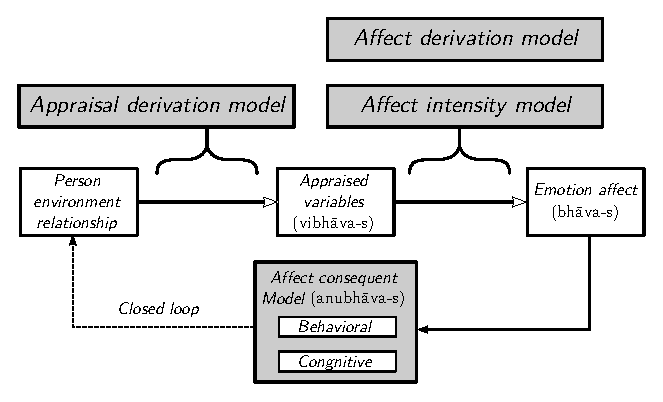
\includegraphics{figures/4.eps}
\caption{A component model view of computational appraisal models (annotated and adapted from Stacy Marsella, Jonathan Gratch, and Paulo Petta, "Computational Models of Emotion", in \textsl{Blueprint for Affective Computing (Series in Affective Science)}, no. 2010, Oxford University Press, Nov, 2010. Original text in italics)}\label{chap7-fig2}
\end{figure}

We therefore start by discussing commonalities across some art forms to rebut Pollock’s claim that there is nothing common (Section \ref{chap7-sec1.3}). We follow with a brief summary of \textsl{rasa} theory (Section \ref{chap7-sec2}) as needed for our purposes. We then give an high level outline of a theory for \textsl{rasa} (Section \ref{chap7-sec3}). We then briefly discuss current theories of mind relevant to \textsl{rasa} (Section \ref{chap7-sec3.1}). We next present an outline of our thesis towards a contemporaneous computational theory of \textsl{rasa} (Section \ref{chap7-sec4}). After, we discuss structuring models in various Indic art forms (Section \ref{chap7-sec4.1}) followed by a computer systems model for \textsl{nāṭya} (Section \ref{chap7-sec4.2}), and end by giving some examples from music in Section \ref{chap7-sec4.3}. Next we discuss computational thinking specifically in the context of poetry (Section \ref{chap7-sec5.1}), music (Section \ref{chap7-sec5.2}), architecture (Section \ref{chap7-sec5.3}) and briefly in some other selected areas (Section \ref{chap7-sec5.4}). We finally end with some conclusions (Section \ref{chap7-sec6}). As to the wellsprings of Indic thinking, we then briefly discuss computational thinking as an important source: first in general (Appendix \ref{chap7-app1}), followed by computational thinking in the Indic tradition (Appendix \ref{chap7-app2}). 

As this paper is very much a work in progress, we hope that future progress in this area find a computational perspective useful.

\subsection{Commonalities across painting and other arts as per \textsl{Citra-sūtra}}\label{chap7-sec1.3}

The \textsl{Citra-sūtra}, a subtreatise of \textsl{Viṣṇudharmottara} on painting and making images, discusses (in Ch. 43) \textsl{rasa}-s in painting based on \textsl{Nāṭyaśāstra}. It begins with king Vajra seeking knowledge from sage Mārkaṇḍeya on the art of making images for worship so that the images manifest the deities. Mārkaṇḍeya says that without knowledge of painting, it is not possible. When he is in turn asked about painting, he says without knowing the dance art form, it is not possible as both art forms require the world to be represented. To learn dance, music, both instrumental and vocal, need to be mastered; then, mastery is also required of classical, vernacular and popular music. Thus painting is needed to understand \textsl{nāṭya}; without knowledge of \textsl{nāṭya}, one can scarcely understand the technique of painting\endnote[22]{It is a humbling or sobering to realize that Shārngadeva has \textsl{pindotpatti} as the 2nd \textsl{prakarana} of the 1st \textsl{adhyāya} in his \textsl{Saṅgītaratnākara} as nāda is produced in the human body, hence the body has to be fully describedfirst!}. 

Furthermore, he says that

\begin{myquote}
“He who does not know properly the rules of \textsl{Chitra} (painting) can scarcely discern the essentials of the images (\textsl{śilpa}).” Also, 

“The observation of nature and of the rules of dancing are indicated as the ultimate resources of the painter. This does not mean that the positions of dancers have to be painted. None of the nine positions of the treatise on painting in the \textsl{Viṣṇudharmottara} coincides with any of the 101 positions explicitly described in Bharata's Nāṭyaśāstra. What is meant by the derivation of painting from dancing is that movement is common to both these expressive forms; it asserts itself in purity through dancing, it guides the hand of the artist, who knows how to paint figures, as if breathing, the wind as blowing, the fire as blazing, and the streamers as fluttering. The moving force, the vital breath, the life-movement (\textsl{chetana}), that is what is expected to be seen in the work of a painter, to make it alive with rhythm and expression. Imagination, observation and the expressive force of rhythm are meant by the legends of the origin of painting, to be its essential features.” 
\end{myquote}

A basic review of the commonality across the various \textsl{kalā}-s is also given by Sreenivasa Rao:

\begin{myquote}
“The Shilpa (sculpture) and Chitra (painting) are closely related to Nāṭya (dance)[...]. The rules of the iconography (prathima lakṣana) appear to have been derived from the Natya-sastra. The Indian sculptures are often the frozen versions or representations of the gestures and poses of dance (cāris and karaṇas) described in Natya-sastra. The Shilpa and Citra (just as the Natya) are based on a system of medians (sutras), measures (mānas), postures of symmetry (bhaṅgas) and asymmetry (abhaṅga, dvibhaṅga and tribhaṅga); and on the sthanas (positions of standing, sitting, and reclining). The concept of perfect symmetry is present in Shilpa and Citra as in Nrittya; and that is indicated by the term Sama.” Furthermore, “The Indian art that rendered religious themes shared a common pool of symbols and avoided imitation of the physical and ephemeral world of the senses. For instance,in all the Hindu, Jaina and Buddhist themes, alike, the Chakra - the revolving wheel of time symbolizes the cyclical rhythms of all existence; the Padma - or the lotus embodies creation - that springs from the bosom of the earth; the Ananta (represented as a snake) symbolizes water - the most important life-giving force from which all life emerges, evolves and then resolves; the Swastika – represents the four-fold aspects of creation, motion and a sense of stability; the Purnakalasha the overflowing pot symbolizes creativity and prosperity; the Kalpalata and Kalpavriksha - the wish-fulfillment creeper symbolize imagination and creativity; and, Mriga - or deer – symbolizes desire and beauty.

Similarly there were a common set of gestures (mudra) by position of fingers, hands, limbs; and by stance of images in paintings and in sculptures. These varied mudras made explicit the virtues such as wisdom, strength, generosity, kindness and caring etc. The objects depicted in Indian art evoked an imagery or represented an idea that sprang from the mind. That might perhaps explain the relative absence of portraiture and even when it was attempted the emphasis was on the ideal person behind the human lineaments rather than on the physical likeness.

Another feature is the absence of the sculptures and other representations of rulers or rich patrons. And, hardly any sculpture or painting bears the signature or the name of its creator. That might again symbolize a move from particular to the universal. But, it surely baffled generations of historians.” (Rao Citra)
\end{myquote}

There is already a hint of \textsl{sādhāranīkaraṇa} of the \textsl{rasa} theory here; we will discuss this in detail later. Additionally, while Pollock concentrates on \textsl{praśasti} to emphasize feudal relations, here we have a different perspective. Furthermore, 

\begin{myquote}
“Indian figurative art is therefore not mere portraiture of the specific; but is a symbol pointing to a larger principle. It is akin to the finger pointing to the moon. For instance the image or the painting of the Buddha could be seen as that of the Buddha the historical prince Siddhartha Gotama and Sakyamuni. But, it is more than that. The Buddha figure is the embodiment of all the compassion, pathos and grace in absolute. Often, certain symbols surrounding the Buddha-image are meant to amplify its message. For instance, the idea of reverence and holiness could be represented sometimes by the surrounding vegetation, flora, fauna, yakshis, gandharvas, and apsaras each playing a specific role in building a totality; or it may be the single austere simple statement of the still centre of peace and enlightenment suggested through the symbols of the Buddha such as the Bodhi tree, seat, umbrella, sandals, footprints etc. The Buddha image is, thus, at once particular and universal. The spirit and soul of the Buddha is contained in the body of the particular but impersonalized form; the serene mood of compassion it portrays is everlasting and universal.” 
\end{myquote}

This again hints at \textsl{sādhāranīkaraṇa} as an important overarching principle. The sacred dimension is also an important common part across various \textsl{kalā}-s. To quote from Stella Kramrisch\endnote[23]{Stella Kramrisch,“\textsl{Vishnudharmottara}, Part III A treatise on Indian Painting and Image Making), 1928 Calcutta”}:

\begin{myquote}
“Vajra said: The Supreme Deity has been described as devoid of form, smell and emotion and destitute of sound and touch so how this form can be (made) of Him? Markandeya replied: Prakrti and Vikrti (come into existence) through the (variation in) the form of the Supreme Soul. That form of Him(which is) scarcely to be perceived is called Prakrti. The whole universe should be known as the Vikrti (i.e,., modification) of Him, when endowed with form. Worship and meditation (of the Supreme Being) are possible (only when He is) endowed with form. The best position of the (Supreme) Soul (however) is to be imagined without form. For seeing worlds (He) possesses eyes closed in meditation... 

This concession being made, life in its entirety becomes fit for artistic representation, and the realm of imagination is as close within the reach of the artists, as nature that surrounds him, for tradition guides him in the one case and observation checks and inspires him in the other. 
\end{myquote}

Interestingly, the cross-\textsl{kalā} aspects are also very much on the table for discussion:

\begin{myquote}
Colour symbolism underlies not only the painting of statues which, according to their sattvika, rajasika and tamasika aspects, had to be painted white, red or dark, but was respectively selected for \textsl{rasa}-Citras, the pictures of emotions, which, according to the Silparatna, formed a group by themselves, distinct from the realistic paintings that were resembling what is actually seen in nature and looked like a reflex in a mirror. Each \textsl{rasa} (emotion) had to be painted in its expressive colour, the Srngara (erotic) was of syama hue, the laugh-exciting (hāsa) of white colour, the pathetic (karuṇa) of grey colour, the furious (rudra) of red colour, the heroic (vira) of yellowish white colour, tho fearful (bhayanaka) of black colour, the supernatural and amazing of yellow colour and the repulsive (loathsome, bibhatsa) of blue colour.
\end{myquote}

Kramrisch says further:

\begin{myquote}
The temple builder and the image maker were working on the same foundation of a magical suggestiveness of form-connections. But the rules valid for both, apply to painting too, as far as they can be applied there. ... This common basis of architecture, sculpture and painting - it was shown that it primarily underliesdancing at times - is responsible for a fusion of the various disciplines of sculpture and painting, for a desperate attempt of visualizing what perhaps is beyond visualisation.
\end{myquote}

The \textsl{Citra-sūtra} concludes with an interesting observation: 

\begin{myquote}
“In this treatise only the suggestions are given, oh king, for this subject can never be described in detail even in a hundred years. Whatever has not been said here should be inferred by other means...” 
\end{myquote}

This observation may be alluding, among many others, to the need for many \textsl{guru-śiṣya paramparā}-s to explore multiple possibilities given the basic structures; this sociological aspect is also common across various \textsl{kalā}-s due to the importance of \textsl{manodharma} in the Indic tradition. 

Considering either Indic philosophy of grammar or \textsl{rasa} theory, there are surprising similarities. In the Indic tradition, the intent (or inner idea, \textsl{sphoṭa}) is said to be the primary cause and then comes elaboration. In the context of \textsl{vāk}, it is elaborated as \textsl{parā}, \textsl{paśyantī} (that which is seen by “seers”), \textsl{madhyamā} (“inner articulation”) and \textsl{vaikharī} (“actually spoken”). In \textsl{rasa}/linguistic theory, we have \textsl{sphoṭa} that corresponds to the 1st two, \textsl{dhvani} that corresponds to the last two. What is interesting is that the commonality arises from the same source or perspective such as, for example, Kāśmīra Śaiva thinking on the nature of reality. Furthermore, Mukund Lath (Lath 2016) in the context of thought and music says 

\begin{myquote}
“...The idea of paśyantī vāk (and the word “vāk” here, can be plainly taken to indicate both music and word-based language: both being sound-based) suggests a level of meaning-consciousness that lies beyond the ordinary levels of language usage, beyond, in other words, of vaikharī (uttered, expressed language) and madhyamā (the unuttered flow of language that keeps endlessly moving in our consciousness). We are in the field of paśyantī when we are seeking to articulate an unexpressed thought—or a rāga. We look for the right word or svara, which is not there but which we reach through our meaning-seeking reflexive consciousness. But what is the criterion of discrimination? The criterion is the unexpressed, disembodied idea itself, for there can be no other. And this search therefore leads us beyond paśyantī into parā: for the sought idea—or rāga—is not a singularly existing “metaphysical” entity, it lies in an ineffable field of an ever creative possibility. This is the parā, the source, the seed or the nucleus of meaningfulness. We have no grasp of it, except, in whatever measure, through our inward-turning reflexive consciousness, which forever and insistently tries to reach out to it.”
\end{myquote}

The above discussion hopefully convinces the reader that lack of commonality is not a defensible proposition and it is incomprehensible that Pollock even makes the charge. We discuss this aspect in a more technical way below by looking at the “atomic” units of the various art forms and how they are grouped bottom up for discussing higher level structures and also the opposite top down view where appropriate.

\section{A Brief Introduction to \textsl{Rasa}}\label{chap7-sec2}

\textsl{Rasa} can be defined as ecstasy derived from seeing or hearing an art form such as \textsl{driśya kāvya} (eg. \textsl{nāṭya}) or \textsl{śravya kāvya} (eg. \textsl{Rāmāyaṇa}). \textsl{Bharatārnavah} of Nandikeśvara in particular says (Gairola 2013)

\begin{quote}
\textsl{aṅgenālambayed gītaṁ hastenārtha-pradarśanam |}\\
\textsl{cakṣurbhyāṁ bhāvayed bhāvaṁ pādābhyāṁ tāla-nirṇayaḥ ||}
\end{quote}

The song is supported by the body

The hands show the meaning

The eyes express the moods

The tala by the feet
\begin{quote}
\textsl{yato hastas tato dṛṣṭir yato dṛṣṭis tato manaḥ |}\\
\textsl{yato manas tato bhāvo yato bhāvas tato rasaḥ ||}
\end{quote}

"Where the hand is, the eyes follow; where the eyes go, the mind follows; where the mind is, there the \textsl{bhāva} is; where there is \textsl{bhāva}, there the \textsl{rasa} is”

The \textsl{anukartṛ} (actor) uses his body (eg. \textsl{grīvā}, \textsl{bhrū}) and \textsl{cāri}, \textsl{karaṇa} (body postures) to emote the \textsl{bhāva}-s. The above \textsl{śloka}-s give a vivid connection between the mind and body coordination so central in a general theory of \textsl{rasa}. A reader or spectator may identify himself/herself with the characters depicted so completely that he/she may weep real tears but it is that of exquisite joy! To explain such a phenomenon, a theory of \textsl{rasa} is needed; this is addressed at length in the Indian tradition. 

In Chap. 6 of \textsl{Nāṭyaśāstra} (6.33-6.34), Bharata says that \textsl{bhāva}-s produce \textsl{rasa} and not vice versa (Rastogi 2016)! However, just immediately afterwards (6.35-37), while Bharata first says \textsl{bhāva}-s cause the many \textsl{rasa}-s through \textsl{abhinaya}, he then says neither is \textsl{rasa} without \textsl{bhāva}-s nor vice versa. Furthermore, in their mutual interdependence, both their fullnesses result from \textsl{abhinaya}; their relationship is like that between a seed and its plant and each causes the other to happen! \textsl{Bhāva}-s and \textsl{rasa}-s cause one another to come into existence (\textsl{bhāvayanti}). These statements can be reconciled if we keep in mind that while at the beginning \textsl{bhāva}-s cause \textsl{rasa}-s to be produced, subsequently, they can have a codependency.

Additionally, a \textsl{rasa} is not a single “essence,” as it is not a single, pure substance but a combination of many sensory inputs; these produce “a richly textured, emotionally resonant experience larger than the sum of its parts” (Beitmen2014). Furthermore, \textsl{rasa} is an additive property. Bharata describes \textsl{rasa} using the metaphor of a mixture: \textsl{rasa} is like the agreeable taste of a well made dish with spices, with the aesthetic experience being the savoring of this dish. Different \textsl{bhāva}-s (emotional states) such as \textsl{hāsya} and \textsl{śṛṅgāra} are like ingredients in the dish; although they are mixed, \textsl{sahṛdaya}-s can distinguish each emotion while at the same time enjoying their creative combination. Bharata’s \textsl{rasa} model is therefore the aesthetics of a mixture of emotions and not pure essences (Beitman 2014). Moreover, Bharata declares that the various \textsl{rasa}-s (the “moods” experienced by the audience members) and the \textsl{bhāva}-s (the “states of being” portrayed by the actors) “cause one another to originate (\textsl{bhāvayanti})”. 

Bharata has listed 56 \textsl{bhāva}-s and 8 \textsl{rasa}-s. For example, \textsl{rati} \textsl{bhāva} and its corresponding \textsl{śṛṅgāra} \textsl{rasa}; similarly \textsl{utsāha bhāva/vīra rasa; śoka/karuṇa; hāsa/hāsya; vismaya/adbutha}. These are \textsl{kāyika} or \textsl{āngika bhāvas}. Examples of \textsl{anangi rasas} are \textsl{bhaya/bhayānaka, krodha/raudra, jugupsā/bībhatsa}; interestingly, some of these are said to be implicated in psychological disorders. Some \textsl{bhāvas} are \textsl{sāttvika} such as \textsl{romanchaka, stambha, vaivarṇya}; these depict the physical expression of the emotions in the mind.

There are primary or stable \textsl{bhāva-s (sthāyibhāva-s)} and secondary or transitory ones (\textsl{sañcāri bhāva-s}). \textsl{sthāyibhāva}-s are stable emotions that can become \textsl{rasa}-s; \textsl{Śrī Bhakti-rasāmṛta-sindhu} (2.5.1) gives the following definition:
\begin{quote}
\textsl{aviruddhān viruddhāṁś ca bhāvān yo vaśatāṁ nayan |}\\
\textsl{su-rājeva virājeta sa sthāyi bhāva ucyate ||}
\end{quote}

“That \textsl{bhāva} which, controlling other favorable \textsl{bhāva}-s such as \textsl{hāsya}, and contradictory \textsl{bhāva}-s such as \textsl{krodha}, presides in the manner of an efficient ruler, is called the \textsl{sthāyibhāva}.” The \textsl{sthāyibhāva}-s are caused to happen by the actor (\textsl{bhāvayanti iti bhāvah}) so that the related \textsl{rasa} is produced in the spectator (\textsl{bhavanti iti bhāvah}); these require, in a good performance, that there is correspondence between the cognitive\endnote[24]{In Indic thought, we have \textsl{manas} (“supervisor” of the 5 \textsl{karmendriya}-s and 5 \textsl{jñānendriya}-s), \textsl{citta} (store of sense impressions), \textsl{ahaṅkāra} (I-am-ness), \textsl{buddhi} (decision maker that may control \textsl{manas}, \textsl{citta} and \textsl{ahaṅkāra}). “Cognitive” here may be taken to be all of these aspects as they deal with the representational aspects. In a computer systems perspective, these are roughly the input-output (I/O) controller, persistent storage, thread of control, and the code/algorithms of the core kernel. Only the network aspect is not explicitly mentioned as it is possibly subsumed by the I/O controller.}/mental states of both the actor and spectator. It is interesting that \textsl{Nāṭyaśāstra} also discusses certain physical states of the spectator in the context of \textsl{rasa} including sounds (claps, counting \textsl{tāla}, \textsl{aho}!, etc) and movements (hands, head, etc); this is an another instance where the Indic world differs in that total silence is not expected from the audience!

\textsl{Viṣṇu-dharmottara} says it in its own way:
\begin{quote}
\textsl{rasānam samavetanam yasya rūpam bhaved bahu}\\
\textsl{sa mantavyo rasaḥ sthāyi śeṣaḥ sancārino mataḥ}
\end{quote}

When \textsl{rasa}-s come together, the \textsl{rasa} whose nature is prominent is the \textsl{sthāyi-bhāva}, and the other \textsl{rasa}-s are \textsl{sañcāri-bhāva-}s.

\textsl{Rasa} is not \textsl{ādhyātimika} but at the same time it is not \textsl{laukika}. Abhinavagupta extended the original 8 \textsl{rasa}s of Bharata by adding \textsl{śānta rasa. Rasānanda} or \textsl{kāvyānanda/kalānanda} is held to be different from \textsl{brahmānanda} but more like \textsl{śānta rasa}; here \textsl{ānanda} is defined as that \textsl{sukha} that is not \textsl{duḥkha-sparśi-sukha} (that which is untouched by sorrow). Later, \textsl{śānta rasa} (Abhinavagupta) and \textsl{bhakti rasa} (Rūpa Goswami/Madhusūdana Sarasvati) have been held to be close to the state of \textsl{mokṣa}. But Bharata’s \textsl{rasa} is in the domain of \textsl{dharma} (\textsl{trivarga}) and not \textsl{mokṣa}\endnote[25]{The Vedas also discuss \textsl{somarasa}; only the \textsl{somarasa} is close to \textsl{śānta/bhakti rasa} and not to others. However, this has been mistranslated as spirituous by European Indologists; this is unfortunate as it is very different from \textsl{madā} (such as \textsl{ariṣṭa or āsava}) (Nagraj 2016).}!\endnote[26]{We briefly list the usage of the word \textsl{rasa} in the \textsl{Trayī} which is different from what we have discussed so far. \textsl{Taittirīya Upaniṣad} (2.7.1) says \textsl{yad vai tat sukṛtaṁ} | \textsl{raso vai saḥ} | \textsl{rasaṁ hy evāyaṁ labdhvā’’nandī bhavati} ||

\begin{myquote}
“That which is known as the self-creator is verily the source of joy [\textsl{rasa}]; for one becomes happy by coming in contact with that source of joy [\textsl{rasa}]” (Gambhirananda 2010)
\end{myquote}

Alternately, \textsl{raso vai saḥ} here has also been translated as “Truly, the Lord is \textsl{rasa}".

Kṛṣṇa in the \textsl{Gītā} says he is the \textsl{rasa} in water, pointing out the subtlety of \textsl{rasa}: not easy to describe (textually?) as it can only be experienced:
\begin{quote}
\textsl{raso’ham apsu kaunteya prabhāsmi śaśi-sūryayoḥ} |\\
\textsl{praṇavaḥ sarva-vedeṣu śabdaḥ khe pauruṣaṁ nṛṣu} ||
\end{quote}

In the earlier thinking on Rasa, like \textsl{asat} (\textsl{asad vā idam agra āsīt} | \textsl{tato vai sad ajāyata} Taittirīya Upaniṣad ***) or \textsl{dharma}, \textsl{rasa} is the seed or alternatively the {\dev योनि} of everything, given its identification with the self-creator or the Lord.}

Bharata says: “\textsl{vibhāvānubhāva-vyabhichāri-saṁyogad rasa niṣpattiḥ}” which is typically translated as follows\endnote[27]{Note some similarity with appraisal theory in the technical area of affective computing (Stacy 2010): “In appraisal theory, emotion is argued to arise from patterns of individual judgement concerning the relationship between events and an individual’s beliefs, desires, and intentions, sometimes referred to as the \textsl{person–environment relationship } (Lazarus 1991) [\textsl{vibhāva}-s]. These judgements, formalized through reference to devices such as \textsl{situational meaning structures} or \textsl{appraisal variables} (Frijda 1987), characterize aspects of the personal significance of events. Patterns of appraisal are associated with specific physiological and behavioural reactions [\textsl{anubhāva}-s]. In several versions of appraisal theory, appraisals also trigger cognitive responses [\textsl{sañcāribhāva}-s?], often referred to as \textsl{coping strategies}--e.g. planning, procrastination, or resignation—feeding back into a continual cycle of appraisal and reappraisal (Lazarus 1991, p. 127).” But the notion of \textsl{rasa} is either not present or not clearly articulated.}: \textsl{rasa} is said to be produced (\textsl{rasa niṣpattiḥ}) by a combination of the \textsl{vibhāva} (determinants), \textsl{anubhāva} (consequents), and \textsl{vyabhicāri-bhāva} (sanchāri or transitory states or fleeting emotions). Some \textsl{vibhāva-}s are \textsl{ālambana} (supporting), some are \textsl{uddīpana} (intensifying; usually environmental ones).

\textsl{Avadhāni} Shankar Rajaraman says:

\begin{myquote}
From an Indian aesthetic viewpoint, narratives can be understood in terms of the emplotment of \textsl{vibhāva}-s (antecedent events), \textsl{anubhāva}-s (consequent responses including verbal and non-verbal behaviours), and \textsl{vyabhicāri-bhava}-s (transient states such as \textsl{garva}, \textsl{asūyā}, \textsl{śrama}, \textsl{vyādhi}, \textsl{viṣāda}). Put simply, Sanskrit poets integrate \textsl{vibhāva}-s, \textsl{anubhāva}-s, and \textsl{vyabhicāri}-\textsl{bhava}-s in a coherent and meaningful manner within a narrative. The effect of emplotment on the reader is that his/her \textsl{sthāyi}-\textsl{bhāva}-s (sustained egocentric mental states such as \textsl{rati}, \textsl{utsāha}, \textsl{śoka}) are transformed into \textsl{rasa}-s - their pleasurable, aesthetic counterparts. According to the \textsl{Nāṭya}-\textsl{śāstra} of Bharatamuni (1992), dramatic narrative (\textsl{nāṭya}) must refer to the actual world for its depiction of antecedent events and consequent responses. \textsl{Vibhāva}-s and \textsl{anubhāva}-s thus have their real world correspondences in the form of \textsl{kāraṇa}-s and \textsl{kārya}-s. To know \textsl{vibhāva}-s and \textsl{anubhāva}-s is to know their corresponding real world \textsl{kāraṇa}-s and \textsl{kārya}-s. \textsl{Vibhāva}-s and \textsl{anubhāva}-s are therefore described by Bharatamuni (p. 153) as \textsl{loka-svabhāvānugata} (compatible with what holds true in the actual world), \textsl{loka-prasiddha} (well-established in the actual world), \textsl{loka-svabhāva- saṁsiddha} (determined by what holds true in the actual world), and \textsl{loka-yātrānugāmi} (in agreement with the world of interactions). The word \textsl{loka} (world) use here refers, no doubt, to a cultural world within which \textsl{nāṭya} is made meaningful. 

\hfill(Shankar 2017) 
\end{myquote}

After Bharata, many thinkers such as Dandin, Bhatta Nāyaka, Ānandavardhana, Abhinavagupta and others discussed the use and application of the theory of \textsl{rasa} to literary texts but with their own innovations. For example, Ānandavardhana introduced a new thinking into \textsl{kāvya} that a poet ought to strive to evoke a single \textsl{rasa}; this predominant \textsl{rasa} he called \textsl{angīrasa}. Even if other \textsl{rasa}-s are necessary, those should be treated as mere auxiliary to the main \textsl{rasa}. Furthermore, a plot also must have a \textsl{angīrasa} with good \textsl{kāvya} avoiding those aspects not directly relevant to the development of the main theme and \textsl{rasa} (such as events, descriptions, figures of speech, etc.). Bharata did not have this requirement: there could be different \textsl{rasa}-s as needed in a dramatic production. Other authors developed this idea further; even here, it seems that each act in a dramatic performance would have a principal \textsl{rasa}. 

As an example, we now give one \textsl{rasa} based analysis in a \textsl{kāvya}, again from Shankar (Shankar 2017):

\begin{myquote}
...[V]erse no. 1.1, the \textsl{nāndī-padya}, of Harṣa’s \textsl{Priyadarśikā}... depicts the marriage between Śiva and Pārvatī, describing a series of emotional states that the latter is going through in that situation. Pārvatī, the bride, longs to have a look at the face of Śiva, the groom. But her eyes are agitated by the smoke from the sacrificial fire. The cool rays of the moon on Śiva’s head come to her rescue and comfort her reddened eyes. Just as she is about to catch a glimpse of Śiva’s face, she beholds Brahmā, the officiating priest, in their vicinity, and out of modesty bends her face down (how could she, in spite of her eagerness, directly look at the groom when another male is standing close by?). She can now see Śiva reflected in her bright toe-nails. But instead of being happy that she could manage to look at least at the reflected image of her husband, Pārvatī is filled with jealousy because along with Śiva is also reflected Gaṅgā, her co-wife, whom he holds in his matted locks. Going through these emotional states, Pārvatī suddenly feels the touch of Śiva’s hand on hers during the ritual of \textsl{pāṇigrahaṇa} and is covered by goosebumps. The poet ends the verse with a prayer that Pārvatī, thus described, bring about auspiciousness....[The] poet has carefully brought together the descriptions of several bodily and behavioral responses (agitated eyes, bending the face down, goosebumps) and mental states (eagerness, bashfulness, jealousy) to strengthen his depiction of Pārvatī’s love for Śiva (In \textsl{Nāṭyaśāstric} terms, the \textsl{sthāyi-bhāva} in this verse is \textsl{rati}, which being augmented by \textsl{vyabhicāri-bhāva}-s such as \textsl{autsukya}, \textsl{vrīḍā} and \textsl{asūyā}, and \textsl{anubhāva}-s such as agitated eyes, bending the face down, goosebumps, etc., is elevated to the state of the \textsl{rasaśṛṅgāra} in the reader.)
\end{myquote}

Another example we can give is that of Lalleśvarī (Lal Ded) of Kāśmīr. In one of her \textsl{vāk-}s, she says (Hoskote 2011):

\begin{myquote}
So many times I’ve drunk the wine of the Sindhu river.

So many roles I’ve played on this stage.

So many pieces of human flesh I’ve eaten.

But I’m still the same Lalla, nothing’s changed.
\end{myquote}

On a first reading, \textsl{bhayānaka} (terrifying) or \textsl{bībhatsa} (disgusting) \textsl{rasa}-s are likely. A deeper explanation is interesting: Lalla’s \textsl{ātman} has used/consumed so many bodies in her past lives!

One cannot fail to notice that \textsl{rasa} is often discussed taxonomically in the Indic tradition (for example, 56 \textsl{bhāva}-s or \textsl{nava rasa}-s); interestingly many of these distinctions are surprisingly well founded (the list of \textsl{bhāva}-s/\textsl{rasa}-s says Patrick Hogan “coincides remarkably well with the lists of “basic emotions” developed by cognitive psychologists in recent years (see, for example, Ekman\endnote[28]{in 1972, Ekman had the following emotions: Anger, Disgust, Fear, Happiness, Sadness, and Surprise. However, in the 1990s Ekman expanded his list of basic emotions, including a range of positive and negative emotions not all of which are encoded in facial muscles. The newly included emotions are: Amusement Contempt, Contentment, Embarrassment, Excitement, Guilt, Pride in achievement, Relief, Satisfaction, Sensory pleasure, Shame (from Wikipedia article on “Affective computing”). Ekman since the last 2 decades has been also working in the area of “microexpressions”.}; Oatley and Johnson-Laird; and Johnson-Laird and Oatley)” (Hogan 2003). The Indic taxonomical impulse is due to its inclusive orientation so as not to exclude anything; Hogan makes an interesting observation on Indian ontology and epistemology that is worth quoting here:

\begin{myquote}
“While all cultures are diverse, India has reveled in its differences. Ancient sages sparred with one another on every question from the meaning of the universe and the nature of soul to the precise number of the varieties of the simile. One may draw a broad distinction between exclusionary cultures and incorporative cultures. Exclusionary cultures tend to identify a “correct” set of practices and to eliminate others. Incorporative cultures tend to accept all varieties of idea and habit, finding a singular place for them — often in a hierarchical structure. Ancient, classical and medieval India are among the most incorporative culturesof which I am aware. Thus, historically, India has been culturally multiple not only in lived culture, but in official culture. Indeed, some of the greatest intellectual achievements of ancient India come from an attempt to systematize that diversity. The theories of \textsl{rasa} and \textsl{dharma} are two primary instances of that systematization.”  

\hfill(Hogan 2003)
\end{myquote}

\section{A High Level Theory for \textsl{Rasa}}\label{chap7-sec3}

In this paper, we argue for a computational cum cognitive basis for \textsl{rasa} as an important component underlying \textsl{rasa}’s theoretical foundations in the Indic tradition and that such a model, we believe, addresses well the issues raised by Pollock above to understand the wellsprings of \textsl{pratibhā} as well as the commonality across \textsl{kalā}-s. For \textsl{rasa}, there is a generation aspect as well as a recognition aspect. For the generative part, the computational cum cognitive aspect is at two levels: at a cognitive level when the art form is performed and at a design level when the art form is created. Also it should be noted that our argument is not only that the \textsl{rasa} felt by a spectator (“at runtime”) has to be partly cognitively structured and therefore supporting cognitive models may be necessary, but also that the creator (“at design time”) needs to understand how to create structures that create the right \textsl{rasa} in the spectator, or the right \textsl{bhāva} that needs to be emoted by the actor or artist and here is where the computational aspect comes in. This is a crucial point that needs to be kept in mind while reading this paper as we are arguing for a non-standard, possibly unfamiliar, perspective. For the recognition part, either the simpler iterative structures are sensed and fused with earlier (emoted) sensations (“\textsl{anubhāva}-s”) by the layman or the more complex probabilistic structures are recognized “emotionally” by the \textsl{sahṛdaya}-s again given earlier \textsl{anubhāva}-s. This aspect is more closely connected with the affective component of \textsl{rasa}, the embodied sense.

Positing a recursive nature of reality (see Kapila Vatsyayan, “The square and circle of the Indian Arts”, Ch.4 for a discussion with respect to \textsl{Nāṭyaśāstra}), a computational/cognitive style of thinking seems to have been the basis of much activity in diverse Indic disciplines. The theory of \textsl{rasa}, in terms of affecting a \textsl{bhāva} in the artists/creators or \textsl{rasa} in the spectators, or constructing the art form in the first place, in turn has had a computational perspective. This is with respect to the wellsprings of \textsl{pratibhā} as well as to understand the commonality across many \textsl{kalā}-s (domains); hence if our argument is sound or well attested by examples in the Indic tradition, Pollock’s imputations above can then be said to be colored by his somewhat consistent negative thinking with respect to Indic models notwithstanding his erudition or overt appreciation in some instances. 

Our main argument for the cognitive component is as follows. As the Indic tradition fundamentally makes a distinction between an actual emotion of being, say, in love or in pain or feel separation (“\textsl{bhāva}”), and what is experienced through \textsl{nāṭya} or music or art, one can say (at the start) that the latter (“\textsl{rasa}”) is a simulation of the earlier one (“\textsl{bhāva}”). As we continue with the performance, each such simulation (using “memory traces” of earlier \textsl{bhāva}-s) has to be stitched together in a larger structure that represents/recalls cognitive states (along with affective states). The notion of “\textsl{dhvani}” builds these ideas further. \textsl{Dhvani} is a non-signifiable (or non-translatable?) "suggestion" of a word, phrase, sentence, (more generally) topic, or a situation constructed linguistically or in some specific art form (but which is quite different from the various \textsl{alaṅkāra}-s considered in poetics). However, one cannot list all the \textsl{dhvani}-s or “suggestions”, even all the pertinent ones, of a given text or performance. Abhinavagupta also says that some memory traces may not be in the foreground consciousness but which may still have an affective component. What is even more interesting are relevant ideas such as sādhāraṇīkaraṇa (“generalization”) that have a computational flavour as we have discussed.

Our main argument for the computational aspect is as follows. The Indic mind, starting from the Vedic and Upanishadic times, conceived of the universe in terms of a recursive structure so that the “very small” and the “very large” could be attempted to be grasped at the same time (see (Kak 2005), (Malhotra 2014))\endnote[29]{For example, in the Sāṅkhyasystem, the \textsl{pinda}-\textsl{brahmānda}concepts map the “microcosm” to the “macrocosm” and vice versa. In \textsl{Atharvaveda} and in AvataṁsakaSūtra, the recursive nature of reality, for example, is thought of as an infinite net with a crystal at each crossing that simultaneously shines light and (recursively) reflects the lights from other lights.}. Mathematically (and computationally), iteration and (more generally) recursion (or its equivalents) are necessary to capture the (Turing) complete potential of a system built on a finite set of rules. This same Indic intuition has been helpful in developing powerful models across many disciplines that deal with \textsl{rasa}. Furthermore, this recursive nature has some surprising or epiphenomenal properties, seemingly not present in the finite set of rules or that are not directly obvious and hence creates a sense of \textsl{rasa} that is exhilarating and worth striving for. (For a brief introduction to computational thinking and its specific Indic aspect, pl. refer to APPENDIX \ref{chap7-app1} and \ref{chap7-app2}). We give some examples of such thinking in some art forms in Section \ref{chap7-sec5}.

Starting from Bhaṭṭa Nāyaka, Abhinavagupta and others, it is argued that \textsl{rasa} or the aesthetic pleasure results from "generalization": the removal of non-essential aspects or the self-interest “which is part of the link between the affect and the representational content in memory traces”. Using what could be called a computational model (viz. computable functions or state machines with inputs and outputs), \textsl{rasa} is said to be “produced” (\textsl{rasa-niṣpattih}) by a combination of the \textsl{vibhāva} (determinants), \textsl{anubhāva} (consequents), and \textsl{vyabhicāri-bhāva} (transitory states or fleeting emotions). By a process of abstraction (called as \textsl{sādhāraṇīkaraṇa} “generalization”), particulars are dropped; this is useful as it is said that common everyday constraints (eg. time, place, person’s emotional moods, etc) limit the experience of \textsl{rasa}. This abstraction allows us to go to the core of the experience itself (a related example in Vedānta is the removal of the “\textsl{avidyā}” clouding our thinking). An analogous method in programming languages is “program slicing” where a program is “simplified” in a consistent way to remove a variable. Furthermore, prototypes have been proposed by later commentators on \textsl{rasa} as a prelude to generalization: for example, male or female as a category instead of a specific character; similarly certain behaviours or situations. The related technique in programming terms is subtyping where a more general type (“generalization”) is used as a formal parameter and any derived type can be passed as an actual. Finally, if the sets of \textsl{rasa}s is finite (as in \textsl{Nāṭyaśāstra}), these \textsl{rasa}s can be considered as the corresponding “equivalent classes” or clusters after the operation of \textsl{sādhāraṇīkaraṇa} or generalization. There are also other mathematical operators in the \textsl{rasa} theory; the rajas and tamas elements of ordinary experience need to be projected out (using, say, “projection operators”) to understand the depths of \textsl{rasa}. When this happens, the subjective aspects also disappear and the ātman enjoys the \textsl{rasa} just as a yogi’s experiences the paramātman (though different qualitatively, it is said).

Bharata discusses, among many others, the question of how to determine the number of experiential states. Are they finite? Also, the question of what is the mapping between the actor’s experiential states to that of the spectator? Interestingly, these states are not held to be the same (“not a one-one mapping”) as they are given different names.

Since one of the primary insights in the Indic tradition is the necessity or importance of a primary \textsl{rasa} along with other secondary \textsl{rasa}s all through an artistic performance, iterative (or recursive) structures are a necessary aspect of a creative work of art so that the repetition or recursion reinforces the main \textsl{rasa} (connections with Orpwood’s theory for qualia can be recalled here). In addition, the notion of “\textsl{dhvani}” requires (Bayesian) updating of cognitive receptive structures (as well as the corresponding affective ones) that are revisited either because real emotions with its intermediate structures are being simulated or the iterative aspect reinduces a dominant \textsl{sthāyibhāva} and its corresponding \textsl{rasa}.

While the Indic tradition insists that \textsl{rasa} is not a cognitive state (there being no subject or object when one experiences a \textsl{rasa}, or equivalently, there is lack of discursive or relational elements; this is also the same intuition that is present in the \textsl{Trayī} as discussed with respect to \textsl{rasa}), it is still useful to have a cognitive model for the various \textsl{bhāva}-s or its simulations as it senses/transits from one “memory trace” to another as cognitive states with associated affective states.

Furthermore, self-referential cognitive structures may themselves be able to capture some aspects of \textsl{rasa} (esp. those intersect with \textsl{alaṅkāra-}s) as discussed in the Indic tradition (eg. in the \textsl{Trayī}) but we do not pursue this here further except to make a note of Kuntaka's \textsl{vakrokti}. This insightful theory posits multiple levels in any linguistic structure and suggests that the tension ({\dev परस्पर स्पर्धा}) between phonetic and semantic levels is mirrored in form and content; a certain “crookedness” in this relation is what makes for an interesting experience or \textsl{rasa}. A simpler form is “\textsl{nindā} \textsl{stuti}” and also irony as we discussed with respect to sentiment analysis. Note that, in a computational setting, a similar model has been attempted by Hofstadter in the 80's at a popular level where he discusses “strange loops” in certain logical, pictorial, genetic, computer or musical systems (Hofstadter 1979). We will discuss later Tymoczko’s orbifields briefly (Tymoczko 2006) and sketch a similar topological model for emotions based on \textsl{Nāṭyaśāstra}.

Note that there are notions similar to \textsl{ākankṣhā} (“expectation”) and \textsl{yogyatā} (“appropriateness”) that are also applicable here; if an aesthetically pleasing (or \textsl{rasa}-filled) iterative or recursive structure is being enacted, the \textsl{rasika} can anticipate certain substructures and that increases the enjoyment.

The two level theory of \textsl{bhāva} and \textsl{rasa}, or the related theory of Orpwood, is conceptually clear and is helpful for further thinking in the domain of \textsl{rasa}. Without such a theory, it is not that easy to express some insights in a straightforward manner. For example, consider Hogan’s explanation: 

\begin{myquote}
“Specifically, the \textsl{dhvani} of a text may now be understood as the schemas, prototypes, and exempla primed or placed in a buffer between long term memory and rehearsal memory. The exempla include not only representational content, but affective force. When an exemplum is sustained in the buffer, its affective force should lead to precisely the sorts of effect hypothesized by Abhinavagupta when he explained \textsl{rasa} in terms of memory traces. Specifically, we have every reason to expect that the affective force of an exemplum would bleed into consciousness without our being aware of its associated representational content, which is to say, the perceptual or propositional aspect of the exemplum. Or, rather, we have every reason to expect this when a set of affectively and representationally related exempla (e.g., sorrowful exempla of love in separation) are maintained in the buffer through repeated priming due to the patterned \textsl{dhvani} of a text.” 

\hfill(Hogan 2003)
\end{myquote}

While insightful, one can see the lack of levels in the description a handicap.

The Indic sense of \textsl{rasa} in addition stresses \textsl{manodharma} of the artist/actor while following these recursive rules. For example, it is said that an expert \textsl{śilpin} (architect) had to know other fields of knowledge such as \textsl{chandas}, music, mathematics, and astronomy. “The various arts and sciences had to be known for the one and the same purpose, so that he could apply them in his work which was to be an image and reconstitution of the universe” (Kramrisch 1928). But this is not enough though. A “perfect” \textsl{śilpin}/\textsl{sthāpati} needs to have “immediate intuition, a readiness ({\dev प्रत्युत्पन्न}) of judgement ({\dev प्रज्ञा}) in contingencies so that, at the end of the construction, is struck with wonder and exclaims “Oh, how was is that I built it?”\endnote[30]{The Karkaraja II copper inscription, 812 C.E. found in Baroda narrates that a great edifice was built on a hill by Kṛṣṇarāja at Elapura (Ellora)and expresses this wonderment of its architect.}” (Kramrisch 1928). This quote is a fine expression of the dynamics between formal recursive structures (to be discussed below) and \textsl{manodharma} that is the hallmark of Indic sense of \textsl{rasa}. We can find similar examples of a musician inspired by \textsl{rasika-}s and/or other musicians on the stage to produce music that while embedded in a formal structure yet can experiment and produce new interesting music.

Since cognitive structures are mental or internal representational models and hence can be part of a computational model, we will from now on in this paper rephrase our model as a computational model of \textsl{rasa} instead of hyphenating the name as computation cum cognition model of \textsl{rasa}. This is possible as we are, at this stage of theorizing, just as Abhinavagupta and many others including Hogan whom we just referred to, assume that the affective states are correlated, at least at a macro-level, with the cognitive structures.

\subsection{Current theories of mind related to rasa and synergistic models}\label{chap7-sec3.1}

As a contrast to the \textsl{rasa} theory, we first give a brief summary of some theories of mind that could be related to \textsl{rasa} and that could be synergistic from our point of view. In current consciousness studies, affective states are said to have qualia (Dennett 1992). We can investigate if \textsl{rasa} is a quale. Four properties are often ascribed to qualia (for example, according to Daniel Dennett): 
\begin{enumerate}
\item \textsl{ineffable}; that is, they cannot be communicated, or apprehended by any other means than direct experience.
\item \textsl{intrinsic}; that is, they are non-relational properties, which do not change depending on the experience's relation to other things.
\item \textsl{private}; that is, all interpersonal comparisons of qualia are systematically impossible.
\item  \textsl{directly or immediately apprehensible in consciousness}; that is, to experience a quale is to know one experiences a quale, and to know all there is to know about that quale. (Quale 2017)
\end{enumerate}

While 1) seems defensible, the whole notion of \textsl{bhāva} and \textsl{rasa} is the attempt to explain or make possible the communication of \textsl{rasa} from an enactor or a creator of an artistic work to the enactee. 2) also has some problematic aspects: Abhinavagupta talks of seven obstacles that prevents one to not experience \textsl{rasa}; this is obviously relational. 3) is also problematic: \textsl{sādhāranīkaraṇa} is an attempt to remove the subjectivity. Finally 4) is also a problem; there being no subject or object when one experiences a \textsl{rasa} (especially. as \textsl{brahmānandasahodara}), or equivalently, there are no discursive or relational elements.

We next briefly discuss axiomatic Tononi \& Koch’s Integrated Information Theory 3.0 (IITv3) model (Tononi 2016) for consciousness to see if ideas of \textsl{rasa} and consciousness are related in this model; IITv3 includes the following central axioms that are “taken to be immediately evident”\endnote[31]{see \url{https://multisenserealism.com/2014/07/07/iit-3-0-central-axioms/}}
\begin{itemize}
\item[1:] Existence: Consciousness exists --- it is an undeniable aspect of reality. Paraphrasing Descartes, “I experience therefore I am”. 
\item[2:] Composition: Consciousness is compositional (structured): each experience consists of multiple aspects in various combinations. Within the same experience, one can see, for example, left and right, red and blue, a triangle and a square, a red triangle on the left, a blue square on the right, and so on.
\item[3:] Information: Consciousness is informative: each experience differs in its particular way from other possible experiences. Thus, an experience of pure darkness is what it is by differing, in its particular way, from an immense number of other possible experiences. A small subset of these possible experiences includes, for example, all the frames of all possible movies.
\item[4:] Integration: Consciousness is integrated: each experience is (strongly) irreducible to non-interdependent components. Seeing a red triangle is irreducible to seeing a triangle but no red color, plus a red patch but no triangle.
\item[5:] Exclusion: Consciousness is exclusive: each experience excludes all others --- at any given time there is only one experience having its full content, rather than a superposition of multiple partial experiences; each experience has definite borders --- certain things can be experienced and others cannot; each experience has a particular spatial and temporal grain --- it flows at a particular speed, and it has a certain resolution such that some distinctions are possible and finer or coarser distinctions are not.”
\end{itemize}

With respect to 1), even if I say, “I experience \textsl{rasa}, therefore it exists”, consciousness is a necessary first step. With respect to 2), Bharata also has an additive model as we have discussed earlier. With respect to 3), the number of \textsl{rasa}-s are said to be finite in the Indic tradition; these may be viewed as equivalence classes out of the many possibilities. With respect to 4), bhāva-s are many while \textsl{rasa}-s are fewer being the result of \textsl{sādhāranīkaraṇa}. With respect to 5), \textsl{rasa} as a \textsl{brahmānandasahodara} is quite different from the consciousness quale as it is close to being universal and hence inclusive. Thus Indic thinking on \textsl{rasa} as a quale is somewhat at variance with the IIT model. In complex domains, it is not clear if axiomatic approaches are effective; if they do, usually it is to synthesize multiple “successful” approaches crying out for a cleaner description. Note that even “simple” software systems display behaviours that cannot be captured “axiomatically”. This is not unexpected as useful axiomatization of even arithmetic for computation is non trivial.

Our thinking is closest to that of Roger Orpwood who suggests that qualia are created through the neurobiological mechanism of re-entrant feedback in cortical systems (Orpwood 2013); this model interestingly corresponds in some of its details to the computational perspective we advance for a model of \textsl{rasa} (for example, in our modelling of \textsl{rasa}, the bhāva-s are akin to information structures and \textsl{rasa} to an information message in Orpwood’s theory for qualia). For completeness, we give the following quote from the wikipedia entry on Qualia discussing Orpwood’s theory:

\begin{myquote}
Orpwood suggests that information in general is of two types: the information structure and information message. Information structures are defined by the physical vehicles and structural, biological patterns encoding information. That encoded information is the information message; a source describing \textsl{what} that information is. The neural mechanism or network receives input information structures, completes a designated instructional task (firing of the neuron or network), and outputs a modified information structure to downstream regions. The information message is the purpose and meaning of the information structure and causally exists as a result of that particular information structure. Modification of the information structure changes the meaning of the information message, but the message itself cannot be directly altered.

Local cortical networks have the capacity to receive feedback from their own output information structures. This form of local feedback continuously cycles part of the networks output structures as its next input information structure. Since the output structure must represent the information message derived from the input structure, each consecutive cycle that is fed-back will represent the output structure the network just generated. As the network of mechanisms cannot recognize the information message, but only the input information structure, the network is unaware that it is representing its own previous outputs. The neural mechanisms are merely completing their instructional tasks and outputting any recognizable information structures. Orpwood proposes that these local networks come into an attractor state that consistently outputs exactly the same information structure as the input structure. Instead of only representing the information message derived from the input structure, the network will now represent its own output and thereby its own information message. As the input structures are fed-back, the network identifies the previous information structure as being a previous representation of the information message. As Orpwood states, “Once an attractor state has been established, the output [of a network] is a representation of its own identity to the network."

Representation of the networks own output structures, by which represents its own information message, is Orpwood's explanation that grounds the manifestation of qualia via neurobiological mechanisms. (Quale 2017)
\end{myquote}

OrchOR (“orchestrated objective reduction”) is an another interesting layered theory, developed by Stuart Hameroff and Roger Penrose, based on quantum processes starting from the intracellular microtubule level (Hameroff 2014). This will be mentioned only briefly here as it makes use of musical metaphors to explain or motivate how consciousness arises (ie. rather than explain how \textsl{rasa} or aesthetics arises)! OrchOR suggests that there is a connection between the brain’s biomolecular processes and the basic structure of the universe and is based on developments in quantum biology, neuroscience, physics and cosmology. For example, it introduces a novel suggestion of “beat frequencies” of faster microtubule vibrations as a possible source of the observed electro-encephalographic (“EEG”) correlates of consciousness.


\section{Outline of a \underline{contemporaneous} Indic theory for \textsl{rasa}}\label{sec4}

Here we give a \underline{contemporaneous} outline of a theory of \textsl{rasa} but which is directly inspired by the deep insights of the early Indic thinkers. The reader is cautioned that much more needs to be investigated for a fuller and a deeper theory but we present it in its current form to further discussion. Such a \underline{contemporaneous} account may be useful in making sense of the diverse perspectives and approaches over the centuries; while there is no claim of diachronic development, we highlight any interesting insights of the early thinkers.

In general, for fruitful communication, both generative models used by the composer/enactor/speaker and comprehension models of the receiver/spectator/hearer are necessary. While Pāṇini focussed on the first (generative) aspect in his study of grammar, a theory of \textsl{rasa} not only needs discussion of both aspects but also in a “cyber-physical-system” (CPS) context necessarily due to its embodied focus, as text is not the only concern. The theorization for \textsl{rasa} has to be necessarily complex as it involves multiple individuals, multiple bodies and a rich and complex communication language. The latter is needed to convey not only the richness and fullness of lived life but also enact imaginary or creative ideas not necessarily congruent to reality (eg. \textsl{Meghadūtam}); anything that obviously falls short is not seriously interesting! Either highly abstract models to capture generality and/or detailed models are necessary. Sangeetha Menon, as an example of the latter, discusses \textsl{abhinaya} through the medium of the eyes in \textsl{Nāṭyaśāstra} along with the nuances of mental states and physical representations (as many as 36 types of eye glances such as \textsl{kānta, dīna, lajjita, glāna} and \textsl{mukula} while there are 21 types of “\textsl{śirobheda}” of the head!) (Menon 2011). These are attempts at inducing a 3rd person (“viewer”) experience through a 2nd person (“enactor”) enactment of what is a 1st person experience or thinking (“author”)!

Furthermore, the spectator has to detach himself from his identity while experiencing the \textsl{rasa}-s by observing the \textsl{bhāva}-s emoted by the actor and following the plot; but this requires control of his body (without getting physically jumpy, for example)! In the case of the actor, there is also the “loss” of his identity, closer “assumption” of the character of the play and with a sufficient control of the body that the character’s body can be emulated to a level that helps in the play rather than distract\endnote[32]{\textsl{Prahlādavijaya} was banned in India a few decades back (‘30s) as an actor actually caused grievous harm while enacting \textsl{ugra} Narasimha. Similarly, in the 2010 movie \textsl{Black Swan}, the actress starts identifying with the swan so much so she slips into “madness” sprouting feathers, her arms become black wings as she finally loses herself and is transformed into the \textsl{Black Swan}. \textsl{Black Swan} can be also interpreted as a Western metaphor for achieving artistic perfection through realism (surprisingly of a phantasy!), with all the psychological and physical challenges one might encounter, i.e. "the film can be perceived as a poetic metaphor for the birth of an artist, that is, as a visual representation of Nina’s psychic odyssey toward achieving artistic perfection and of the price to be paid for it.” (sentence partially paraphrased from wikipedia’s article on the movie)}. Menon says 

\begin{myquote}
“The actor has to play the twin role of ‘being the character portrayed’ and also the narrator of the story. It is this twin and contradictory role played by the actor which enables the spectator to have the experience of \textsl{rasa}which also involves an interesting contradiction. Unless the spectator can be one with the mental state of the character portrayed s/he will not be able to appreciate the story and the specific nuance. At the same time unless a continuous detachment is maintained s/he will not be able to integrate the experience of that nuance in relation to his/her self-identity”. 

\hfill(Menon 2011)
\end{myquote}

Such requirements may be satisfiable through many differently conceived models and hence there are many arguments in the texts on which model is likely to be true. Using a computational model, one can attempt to show how some of the “contradictions” listed above can be “avoided” or sidestepped\endnote[33]{Interestingly, some interesting conundrums in computer science (such as scheduling in operating systems (OS), recovery of faults in distributed systems, assumption of state by a survivor of the state of the failed unit, etc) are surprisingly related to this same situation! For example, in highly available systems, failure in any part is masked typically by a replicated functioning component elsewhere. On failure of one part of a replicated set, its communications in flight at the time of failure may be redirected to the functioning part in some designs. Now this part has to have two personas: itself and that of the failed (emulated) one; each communication received has to be disambiguated and posted to the correct persona. Otherwise, the system will not work correctly. Similarly, there can be “mode confusion” in such systems when incorrectly tagged data arrives and acted upon wrongly. In dance dramas, this mode confusion may also take place; not only at the actor level but also at the spectator level: a good example is the worship/popularity of actors enacting Indic heroes such as Rāma. The problem of scheduling in OS is related as when the same actor is expected to enact one emotion and then another; this can be cast as the problem of “scheduling new emotions”. The philosophical issue is whether there is an “inner controller” that directs the assumption of various emotions; this is feasible if there are independent multiple threads of execution (and not multiplexed). If multiplexed, it is not feasible as an independent inner controller cannot exist due to “\textsl{anavasthā}” (infinite regression)! The basic problem is that if the inner controller also needs to get control of the execution to do the scheduling (due to the multuplexing), we have not solved the problem as it is the same recursive problem to get the control. This issue is also similar to the problem of whether such an inner controller exists in deep sleep as argued by Yogin-s, Vedāntin-s, Naiyāyika-s, and Buddhists (for details, see (Thompson 2015)).}. However, such a solution may also need to make some deep philosophical assumptions\endnote[34]{For example, a reasonably complete theory of \textsl{rasa} is necessarily connected with the issue of consciousness. Current theories of consciousness are widely divergent; for example, “computationalism” of Dennett (Dennett 1992) and “integrated information theory” of Tononi et al. (Tononi2016) start from opposite ends. While the first “explains away” consciousness as an epiphenomenon (and therefore rasa may also be completely explained in a “bottom up” fashion), the latter takes consciousness to be a starting point for explaining the connection between mind and body just as in Vedantic thinking or later thinkers in the West such as Rene Descartes using a different perspective. The latter Vedantic perspective is also closer to Indic thinking in the \textsl{rasa} domain as intent/suggestion/\textsl{sphoṭa} and \textsl{dhvani} are in the picture. We will later also briefly touch upon Orpwood’s theory of reentrant feedback circuits for explaining qualia as it is closer to our modelling for \textsl{rasa}.} as we are not yet in a position to locate or find neuro-correlates experimentally. Furthermore, such a model may possibly also be used to explain some of the pathologies of communication seen (such as autism).

If we are working towards a computational model of \textsl{rasa}, we need to clearly clarify why we are not calling it a mathematical model. While computer science has often been called “constructive mathematics”, current mathematics has a strong bias towards clear definitions/deep generalizations, theorems/lemmas, proofs and therefore may not reveal its strengths in disciplines with strong phenomenological aspects (eg. current understandings in neuroscience and even in quantum physics (for example, particle physics phenomenology) or the subject matter of \textsl{rasa} itself here. In phenomenological explanations, provisional models are built and checked for correspondence with experimental results; interestingly, the Indic thinking is closer to this way of thinking (see Appendix 2 for details). While the models built are necessarily intended to reveal some aspect of reality, they can be changed and newer models investigated as they do not claim to represent reality completely. This mirrors the extensive debate between axiomatism and computational perspectives (see Appendix \ref{chpa7-app1}). 

Since a critical aspect of \textsl{rasa} is that it requires a performative aspect (such as dance, music, painting, reading/hearing text, viewing (or replaying in one’s mind) some piece of art), there is a generative aspect and a communicative aspect. Considering the communicative aspect first, there can be two aspects: cognitive and affective. Cognitive aspects can be modelled computationally with sufficient detail (if not feasible with just simple mathematical structures), and interactions between objects that have ontological status can be distilled into code\endnote[35]{Note that denotational semantics attempts to model a program as a set of mathematical objects using lattices, etc (eg. Dana Scott) while concurrency may use topological models for insights (eg. Herlihy).}. The generative aspect is necessarily constructive and therefore there is an element of design. Even if the subject matter is not understood well enough, deep insights can be laid down as provisional “constraints” in the system and passed down from teacher to students. We discuss a few examples such as the mathematical basis of Indian cuisines using a multi-dimensional space for the flavours, or in the context of music in two different traditions. For Western classical Music, Dmitri Tymoczko\endnote[36]{see, for example,Youtube video, \url{https://www.youtube.com/watch?v=XUyx31f-U3M}} distills some of these insights into a mathematical model and explains why, for example, Chopin is enjoyed by many whereas avant garde music is only appreciated by a few (see below). Similarly, Indian Music is well known for its \textsl{guru-śishya paramapara} or its many different “\textsl{gharānas}” to transmit across generations some “unformalized” deep understandings such as how to render microtones (\textsl{gamaka}-s) so critical to its imagination.

\section*{Why Computational?}

What then constitutes a computational (or equivalently a constructive mathematical) model for \textsl{rasa}?
\begin{itemize}
\item[(i)] “Generative” modelling Help in searching for domain-specific patterns that produce \textsl{rasa}: the simpler mathematical/combinatorial (eg. enumerating \textsl{tāla}-s (eg. Pingala) or \textsl{raga}-s (eg. Venkatamakhi’s \textsl{melakarta} scheme)) vs (inescapably) computational (in Western classical music, eg. searching for what chord changes are useful or pleasing? in Indian music, eg. how to induce a mood, context sensitive rules about how to decide \textsl{vādi} and \textsl{vivādi svara}-s, transitions between \textsl{svara}-s in the context of a \textsl{rāga}). In the context of text, it could be simple or deeply “linearized” structures, sometimes with multiple levels of recursion (\textsl{Panchatantra/Hitopedesa/Dasakumara Charitra }and even with multiple entries/exits of the author Vyāsa/Vālmikī himself\endnote[37]{There are also stories of complete virtual simulation such as in \textsl{Bhāgavatam} where Brahma is fooled by the boy Kriśna.} as in \textsl{Mahābhārata}/\textsl{Rāmāyaṇa}, along with multiple (recursive) reciting levels) or “chorded” stories where multiple events/narratives run concurrently but presented linearly textually by interleaving them (which is quite common nowadays: eg. “The Joke” by Milan Kundera) or, even more impressively, as \textsl{Citrakāvya} (eg. \textsl{Rāghavapāndavīya} of the twelfth-century poet Kavirāja that tells the story of \textsl{Rāmāyaṇa} and the \textsl{Mahābhārata} simultaneously through ingenious \textsl{Śleṣa}). Or plain stream of consciousness writings such as by Joyce. Interestingly, the \textsl{alaṅkāra-}s (similes, for example) used in \textsl{kāvya-}s typically have a stylized representation in \textsl{nāṭya}. For Indic architecture, pl. see sec \ref{chap7-sec5.3} where we discuss some discussion of the mathematical structures involved; note that even here \textsl{Śleṣa} may have been deliberately attempted, as in Mahābalipuram where certain aspects of the (said by some to be possibly world's largest narrative) sculpture panel favour Arjuna’s penance for the boon of \textsl{Pāśupata astra} and others Bhagīratha’s penance to bring down Gaṅga. In this paper, sec \ref{chap7-sec5} discusses further the generative aspect in four art forms.

\item[(ii)] Descriptive (eg. how to recognize \textsl{rāga}-s/\textsl{rasa}-s with statistical, machine learning models; in Indian music, \textsl{svarasthāna}-s vs reality of \textsl{svara}-s\endnote[38]{see, for example, TM Krishna’s talk, \url{https://www.youtube.com/watch?v=ue7TypsHCV4}}), taxonomy of \textsl{rasa} (ontological models), or even “diachronic” models of \textsl{rasa}. In this paper we discuss the taxonomy aspect as necessary.

\item[(iii)] How does the affective part arise in the first place? How different is it from, for example, the cognitive part? ie. can one explain the affective part as an epiphenomenon? Can \textsl{rasa} also be modelled in a computational theory of mind? This is a complex subject and we have discussed it in sec \ref{chap7-sec4.1} primarily but also touch upon it in many other sections.

\item[(iv)] Computational help in modelling \textsl{rasa} itself (“architecture”, atomic units, levels of description, interconnections amongst units and across levels, epi-phenomenonal aspects, ...), correspondence with neuro-correlates by experiments typically attempted in computational neuroscience. The first part is discussed in this section (sec \ref{chap7-sec3}) and the next (sec \ref{chap7-sec4}); the second part is discussed in brief descriptively if at all.
\end{itemize}

A fruitful model should be able to predict or explain some aspects that were not possible without such a model; however this might be ambitious as of now. A computational model may also be congruent to Indic sensibilities. As discussed before, there is a strong “anti-realist” position in Indic thinking, with \textsl{vyañjanā} (suggestion) as the basis of art. From a computational perspective too, one can argue that “perfection” is a chimera especially in complex domains (such as perfect shapes and the like in Greek thinking and later) and what is useful is a “sufficient” model that conveys what needs to be conveyed/suggested and which can be approached or approximated through a process of iteration\endnote[39]{with such a perspective, Zeno’s paradox, irrationals, infinitesimals and the like are not “showstoppers” as it happened for quite some time in the Greek/European mathematical thinking}. In this connection, we observe that a “computational positivism” perspective informed much of Indic thinking in sciences (see Appendix \ref{chap7-app1} and \ref{chap7-sec2}) and it is useful to think of this perspective in art forms too as Indic thinking typically looked for connections across disciplines.

In our tradition, taking music as an example, production of sounds has a long history (viz. Pāṇini and \textsl{sandhi}) and also discussed, for example, as \textsl{pindotpatti} by Sārngdeva. Locality properties are involved in \textsl{sandhi} as they reflect the anatomical structures of the speech-producing organs; similarly, production of \textsl{svara}-s have certain constraints with respect to what svara-s have been rendered before (as we do not have harmony with multiple voice leadings; but even here locality is important as we discuss below). The constraints can be coded in multiple ways; in Indian music, it was formalized partly as \textsl{ārohana} and \textsl{avarohana} in the system of \textsl{rāga}-s that emphasized melody and microtones. Indian music specially deals with the space between tones (viz, microtones). Even though there are many unifying principles behind a \textsl{rāga}, ultimately each individual defines a raga for himself even after adhering to an accepted framework: how \textsl{śruti}-s are handled is very individualistic within the narrow spectrum of freedom available. The difference between a pure note and a \textsl{śruti} is a “dance” between form and formlessness, or certainty and ambiguity\endnote[40]{Some of these insights are from a talk by PurnaprajnaB. talk at NIAS 2018}. Instead of \textsl{svara} being taken strictly as an interval (suitable for beginners?), \textsl{svara} is seen by experienced musicians as a range that depends on the context of, especially, the \textsl{rāga}, ie, it is seen as a melodic idea rather than as an independent entity. With \textsl{gamaka}, for example, a \textsl{svara} might cross multiple nominal \textsl{svarasthāna-}s; furthermore there are instances where 2 equivalent \textsl{svarasthāna}-s (eg. {\dev री}2 and {\dev गा}1) are disambiguated depending on the context of the \textsl{rāga}.

To further explicate the computational aspects in art forms, an instructive example is the recent discovery of the basis of diversity of recipes in Indian cooking (Jain 2015) where the researchers have found that “in contrast to positive food pairing reported in some Western cuisines, Indian cuisine has a strong signature of negative food pairing; more the extent of flavor sharing between any two ingredients, lesser their co-occurrence” with “spices, individually and as a category, form[ing] the basis of ingredient composition”. Using flavour as the “determinant”, they considered various molecules involved in a flavour. Using an averaged measure of the shared flavours (in terms of molecules) across all the ingredients, it has been found that this measure in Indian cuisine is significantly lesser than expected by chance. What this means is that if ingredients are categorized by flavours in a multi-dimensional space, the ingredients are chosen that are not local in terms of distance in that space (eg. curds and pickles); contrarily, Western cuisine prefers locality (for eg, milk and bread). For aesthetics, the question is then: is there a multi-dimensional space for entities in each art form (or their combinations) in terms of ontologically relevant features, along with a preference model for composition of entities in terms of distance (eg. near: local, far: non-local, intermediate: semi-local)? We give such a model for Bharata’s \textsl{rasa} model based on the description in \textsl{Nāṭyaśāstra} below. It is interesting or curious that Bharata uses mixing of ingredients in cooking to explain \textsl{rasa}-s!  

Furthermore, recent work in understanding the basis of Western music also points in a similar direction. In contrast to Indian music, Western Music deals mainly with polyphony, counterpoint and key changes; it was discovered post 16th century that chord progression had to have some locality constraints for it to be pleasing. Dmitri Tymoczko postulates, for example, some high level desirable principles such as local transformations (eg. transposition: C Major chord to F major chord) or inversion (eg. C major to F minor) (Tymoczko 2006). Using these, he constructs topological objects called orbifolds: those movements in this structure that are local (“nearby”) are generally pleasing. He surmises that Western Music composers such as Mozart/Chopin intuited these resulting in music that has survived till today (in one popular composition, for example, Tymoczko shows that Chopin systematically traverses, one by one, all the “local” paths from a “top” chord in the orbifold space) but later composers experimented without such constraints with mixed results. Basically, exploiting such topological spaces may be difficult or even non-intuitive if local constraints are violated. For example, R Jourdain, a composer and pianist, says with respect to developments in harmonic music (Jourdain 2008): 

\begin{myquote}
p.98: [post Debussy/Strauss 1850’s] "The brain’s powers of harmonic discrimination had been pushed to their limits, as had the powers of short-term memory that maintained tonal centers long after they had faded from the aural stage. Music became harder and harder to appreciate. In view of some critics, it had become altogether inappreciable.” 

p. 100: “Today, concert audiences obediently sit thru music by Schoenberg and his followers, but few enjoy it. Although there is much that is interesting in this music, people do not find it harmonious. It hurts their ears.”\endnote[41]{Constrast this with the spontaneity and enjoyment of music by both the performer and \textsl{rasika} in Indic music systems as locality (as defined by \textsl{ārohaṇa}/\textsl{avarohaṇa} but not too close to avoid nearby dissonant \textsl{svara}-s) and various types of microtones (\textsl{gamaka}-s) are employed extensively. Even today, meditative music is usually associated with \textsl{rāga}-s; an informal poll of some acquaintances trained in the Western tradition of classical music also confirms the immediacy and accessibility of \textsl{rāga}-s; also George Harrison says:

\begin{myquote}
Indian music is brilliant and for me, anyway, (this is only personal) it's got everything in it. I still like electronics and all sorts of music if it's good but Indian music is just... an untouchable you can't say what it is, because it just is.
\end{myquote}}

p. 114: "The key to absolute pitch is early training - very early training [4 years or younger!]... Those who learn itlater... report mixed results... skill tends to ebb away once practice ceases...”
\end{myquote}

\section*{Modelling Emotions as per \textsl{Nāṭyaśāstra}}

As an example, let us now consider the modelling\endnote[42]{Note that the Indic model has both the discrete and dimensional perspective as understood in the current theories in affective computing (Gratch 2009): “Theories differ in which components are intrinsic to an emotion (e.g., cognitions, somatic processes, behavioral tendencies and responses), the relationship between components (e.g. do cognitions precede or follow somatic processes), and representational distinctions (e.g. is anger a prototype or a natural kind). For example, discrete emotion theories argue that emotions are best viewed as a set of discrete sensory-motor programs (Ekman, 1992; LeDoux, 1996; Öhman \& Wiens, 2004). Each of these programs consists of a coherent brain circuit that links eliciting cognitions and somatic responses into a single neural system. At the other extreme, dimensional theories (e.g., Russell, 2003) argue emotions are simply cognitive labels we apply retrospectively to sensed physiological activation, which, rather than consisting of discrete motor programs, is characterized in terms of broad bipolar dimensions such as valence and arousal (e.g. I feel negative arousal in a context where I’ve been wronged, therefore I must be angry).”} of \textsl{Rasa}s as per \textsl{Nāṭyaśāstra}. There are 8 \textsl{rasa}-s (obviously we do not include the \textsl{śānta rasa} here), 8 \textsl{sthāyi bhāva}-s, 33 \textsl{sanchāri bhāva}-s and 8 \textsl{sāttvika}. As discussed earlier, \textsl{vibhāva}-s and \textsl{anubhāva}-s together with \textsl{sanchāri bhāva}-s are conventionally said to give rise to \textsl{rasa}; alternately, \textsl{sthāyibhāva}-s are said to give rise to \textsl{rasa}.

According to this text, the 8 \textsl{rasa}-s (and its corresponding \textsl{sthyāyī bhāva}) have a relationship of transformation through a specific type of action as given below (along with the colour changes):
\begin{enumerate}
\item \textsl{śringāra} (\textsl{śyāma}) $\to$ (mimicry) \textsl{hāsya} (\textsl{sita}) light green $\to$ white

\item \textsl{raudra} (\textsl{rakta}) $\to$ (result act) \textsl{karuṇa} (\textsl{kapota}) red $\to$ ash

\item \textsl{bībhatsa} (\textsl{gaura}) $\to$ (results in seeing) \textsl{bhayānaka} (\textsl{kṛṣṇa}) light orange $\to$ black

\item \textsl{vīra} (\textsl{nīla}) $\to$ (result act) \textsl{adbhuta} (\textsl{pīta}) blue $\to$ yellow 
\end{enumerate}

For example, the first one says that \textsl{śringāra} (its \textsl{sthyāyī} \textsl{bhāva} being \textsl{śyāma}) thru mimicry becomes \textsl{hāsya} whose corresponding \textsl{sthyāyī bhāva} being \textsl{sita}; colourwise, it is a change of the associated \textsl{rasa} colour of light green (or black) to white. Independently, the text says that \textsl{śringāra} and \textsl{karuṇa} (pathetic) seem related (esp in the context of lovers) but one is of optimism vs despair of the other. 

Next, the consequents for each \textsl{rasa} are listed in \textsl{Nāṭyaśāstra} as: 

\textsl{śṛṅgāra}: defined negatively as without fear, indolence, cruelty or disgust

\textsl{hāsya}: indolence, dissimulation, drowsiness, sleep, dreaming, insomnia, envy

\textsl{karuṇa}: indifference, languor, anxiety, yearning, excitement, delusion, fainting, sadness, dejection, illness, inactivity, insanity, epilepsy, fear, indolence, death, paralysis, tremor, change of color, weeping, loss of voice

\textsl{raudra}: presence of mind, determination, energy, horripilation, trembling indignation, restlessness, fury, perspiration

\textsl{vīra}: contentment, judgement, pride, agitation, energy, ferocity, indignation, remembrance, horripilation

\textsl{bhayānaka}: paralysis, perspiration, choking voice, horripilation, trembling, loss of voice, change of color, fear, stupefaction, dejection, agitation, restlessness, inactivity, fear, epilepsy, death

\textsl{bībhatsa}: epilepsy, delusion, agitation, fainting, sickness, death

\textsl{adbhuta}: weeping, paralysis, perspiration, choking voice, 

horripilation, agitation, hurry, inactivity, death

Given the above, one can list each such \textsl{bhāva} as a vector of mental and physical “basic” states (voluntary or involuntary) and also come with some metric of distance between emotions. Since crying, taken as an example, seems to result due to extreme happiness or extreme sadness\endnote[43]{According to current research, the hypothalamus cannot distinguish between being happy or sad or overwhelmed or stressed as it gets a strong neural signal from the amygdala (which registers our emotional reactions) and that it, in turn, activates the autonomic nervous system responsible for the tears. Furthermore, there are different centres in the cortical brain that deal with these emotions; one can feel both at the same time (as in bittersweet memories).}, without the \textsl{vibhāva}-s, we cannot discriminate them due to the identical mapping of the emotions to the same \textsl{anubhāva}. Taking such cases (as well as a neurological mapping of emotions if also available\endnote[44]{Now possible with techniques such as positron emission tomography(PET) or fMRI. Many constraints have a neural basis (like color, pitch).} as per current understanding), the vector can be suitably modified to reflect nearness or identity of some states. Furthermore, from a composer’s perspective, \textsl{vibhāva}-s and \textsl{anubhāva}-s need to be sequenced appropriately to avoid confusion (similar to \textsl{vivādi} \textsl{svara}-s)

Furthermore, Abhinavagupta using Sāmkhya psychology (“sublime”: \textsl{sattva}, “restless”: \textsl{rajas}, “stupid”: \textsl{tamas}) says

\begin{myquote}
“aesthetic emotion is of the nature of \textsl{visrānti} (serenity) of the heart/spirit a condition in which restlessness attendant upon mundane activity is stilled by the play of artistic presentation ... [while] sorrow is the outcome of the restless disposition of passion but, thanks to artistic presentation, the sublime disposition of purity dominates over it and sublimates the tragic situation.” 

\hfill(Raghavan 1961)
\end{myquote}

Such insights can further be added to our model by additional transitions that can be marked as local in the context of aesthetic emotion: the notion of \textsl{sādhāranīkaraṇa} but now with a \textsl{Sāmkhya} perspective. Such additional rules may induce “twists” or even loops in the abstract space just as in Tymoczko’s model where, for example, the chord frequencies form an unordered set rather than an ordered sequence.

The topological structure that results can possibly be used to see how natural it is for transitions between emotions. One can surmise that “localized” transitions are more realistic in a performance just as in music with localized changes (eg. in the context of \textsl{ārohana}/\textsl{avarohana} in Indic music but avoiding dissonant \textsl{svara}-s judiciously even if near, and chord progressions in Western music); also, what are forbidden or discouraged transitions (which sometimes could be actually close in the abstract space). With non-local transitions, discordant emotions or \textsl{rasa}-s are likely to be primary. If we consider music, we can discern 2 major styles: fix pitches as in Western music and look for localized chord progressions and voice leadings (equivalent to locality in orbifold space), or, work with relative pitches as in Indian music and look for local movements (constrained by \textsl{ārohana}/\textsl{avarohana}) using complex melodic ideas such as highly ornamented \textsl{svara}-s that are not just plain \textsl{svarasthāna}-s fixed in relation to the tonic. Note the difference with the earlier \textsl{mūrchana}-s that also used transpositions but in a non-tempered scale\endnote[45]{The earlier music before \textsl{rāga} system was based on meter and close to \textsl{sāhitya}; one had to choose meter to express emotion (eg. playfulness with \textsl{śārdūla-vikrīḍitam}).}. Note further that even in Indian music, when melody is accompanied with a (tonal) rhythmic instrument such as \textsl{mridaṅgam} or tabla (see Sec 5.4), structures similar to orbifolds can be used for description\endnote[46]{Kuntaka discusses \textsl{vakrokti}: this may be due to “loopiness” in the topological structure where levels have got get collapsed or become near (due to a Mobius twist, for example).}. Due to the notion of improvisation, however, these cannot be fixed structures; even then, certain structures will be conserved across\endnote[47]{vide our earlier remark of structures such as “profile HMMs”}, for example, \textsl{gharāna}-s so that meaningful communication is possible. Contrast this with Western music that is based on a fixed notation, and hence valorises “inspired” reproduction but with minimal or no “probability” aspects; variety now comes with new compositions Again, we can see that Indian thinking/art revels in “suggestion” (\textsl{vyañjanā}) and not completely fixed and formed entities.

Having discussed what a computational model can entail, we next discuss atomic units in communication, followed by the grouping of such units, the semantics of such groupings, the possible generative model for the linguistic (L) objects, cognitive (C) states as well as affective (A) states (L+C+A) given the need for comprehension by a general audience as well as by \textsl{sahṛdaya}-s, the transmission of the these L+C+A units from the creator of the art work, to the enactor and then to the spectator/audience, the recognition model of the received symbols by the enactor from the composer/creator and by the audience/spectator from enactor.

\subsection{The “atomic units” in various art forms and higher-level structures}\label{chap7-sec4.1}

Each major \textsl{kalā} in the Indic tradition has a reasonably well developed structural model. Pāṇini’s astounding success on codifying Sanskrit grammar is likely to be the inspiration; for example, in the area of linguistic analysis, after Pāṇini, there has been original progress in the various layers or domains of phonetics, phonology, morphology, syntax, semantics, and pragmatics. Such a layered system was possibly inaugurated by Pāṇini with his \textsl{Māheswara} \textsl{sūtrāṇi} that is based on sound phonological principles; his grammar however only discusses formation of words using recursive rules and does not seriously discuss analysis of sentences or semantics. Using Pāṇini’s example and deep insights, later \textsl{śāstrakāra}-s investigated higher layers such as semantics (in “\textsl{ārthika} \textsl{grantha}-s” such as \textsl{Vākyapadīyam}, \textsl{Vaiyākaraṇalaghumanjūṣa}, \textsl{vaiyākaraṇabhūṣaṇa}(-\textsl{sāra})) and \textsl{rasa} (such as the use of ideas in \textsl{Vākyapadīyam} to \textsl{rasa} in \textsl{Dhvanyāloka}). What is interesting is also philosophical discussions on whether lower layer units combine to give higher layer structures, whether higher level intention structures lower level units, or whether there are epiphenomenal aspects (anticipating the much later developments in computer science of the concepts of synthetic and inherited attibutes of attribute grammars\endnote[48]{It is interesting that D E Knuth, a celebrated CS researcher, says he was not aware of the possibility of inherited attributes in the analysis of computer languages till a researcher suggested it to him! (Knuth 1968)}.

Ānandavardhana and Kuntaka discuss whether literary texts signify any thing other than the word meanings, similar to the discussion of {\dev अभिहितान्वित} vs {\dev अन्विताभिधान} ({\dev अभिहित:} “fixed” {\dev अन्वित:} connected {\dev अभिधान:} saying) in {\dev मीमांसा} and related areas. Computationally, this is the difference between the semantics of processing linguistic structures strictly bottom up or “topdown” (or in a “loopy” way); this is now at the \textsl{rasa} level instead of at the linguistic level. As V.S.Apte says (in the entry on \textsl{abhidhā} in his “Sanskrit Dictionary”):

\begin{myquote}
The \textsl{abhihitānvayavādin-}s (the Bhāṭṭas or the followers of Kumārilabhaṭṭa who hold the doctrine) hold that words by themselves can express their own independent meanings which are afterwards combined into a sentence expressing one connected idea; that, in other words, it is the logical connection between the words of a sentence, and not the sense of the words themselves, that suggests the import or purport of that sentence; they thus believe in a \textsl{tātparyārtha} as distinguished from \textsl{vākyārtha}. The \textsl{anvitābhidhānavādin-}s (the \textsl{Mīmāṁsaka-}s, the followers of Prabhākara) hold that words only express a meaning ({\dev अभिधान}) as parts of a sentence and grammatically connected with one another ({\dev अन्वित}); that they, in fact, only imply an action or something connected with an action; e. g. {\dev घटम्} in {\dev घटम्आनय} means not merely 'jar', but 'jar' as connected with the action of 'bringing' expressed by the verb.
\end{myquote}

If we consider dance forms, both \textsl{Nāṭya-Darpana}/śāstra (of Nandikeswara and Bharata respectively) describe various \textsl{mudra}-s (hand gestures) to convey different ideas; from a finite set of these, the grammar of the \textsl{mudra}-s generates a vast set of suggestive ideas that in principle covers almost all the aspects of human life and the “universe”. Hence \textsl{mudra}-s form the basis or ‘basic units’ of an expressive language; they also give an unique poetic sensibility while performing \textsl{abhinaya}.

Thus, if one does even a cursory study of the various \textsl{kalā}-s (art forms), it becomes clear that Indian theoreticians thought of each \textsl{kalā} as a multi-layered system. The basic units at the lowest layer for poetry/\textsl{chandas}/\textsl{kāvya} are \textsl{gana}-s; for music: \textsl{svara}-s (for \textsl{rāga}) and \textsl{gana}-s (for \textsl{tāla}); for dance: \textsl{mudra}-s, \textsl{svara}-s, \textsl{gana}-s; and for sculpture: “frozen” \textsl{mudra}-s and so on. Even here, there are interesting complexities: for example, taking the case of poetry, there are three aspects or powers of words in the Indian linguistic philosophy. First, the \textsl{abhidhā} (denotation) of a word, lexical meaning in ordinary language, followed by the \textsl{lakṣanā} or \textsl{gaunī} (the secondary sense or the metaphorical one). The third one is the \textsl{tātparya} (intention) by which the separate word-meanings/\textsl{abhidha} are connected together to generate a contextual \textsl{vākya}-meaning. Later \textsl{dhvani} (suggestive meaning) is given as fourth power; Abhinavagupta, who wrote \textsl{Lochana}, a detailed commentary on the \textsl{Dhvanyāloka} says: “\textsl{Caturthyam tu kaksayam dhvanana-vyapara}” (\textsl{Lochana} I.4). This suggested meaning is also known as \textsl{vyañjanā}.

In \textsl{sphoṭavāda}, each \textsl{pada}/word is not taken into account separately after splitting a \textsl{vākya}/sentence. \textsl{Sphoṭa} is perceived only after the sound of the last word is combined with the sensory impressions produced by the earlier words. Similarly, \textsl{dhvani} “echoes” the suggested meaning by integrating all other forms of meanings - \textsl{abhidhā}, \textsl{lakṣana} or \textsl{tātparya}. Just as there is a \textsl{krama} (sequence) through which a word indicates its meaning, there is also a \textsl{krama} through which the \textsl{dhvani} is revealed. In grammar, the sequence is from sound to word, from word to \textsl{sphoṭa} and from \textsl{sphoṭa} to meaning. In poetic creations, the \textsl{krama}\endnote[49]{Ānandavardhana uses \textsl{saṁlakṣya-krama} for non-\textsl{rasadhvani}-s and \textsl{asaṁlakṣya-krama} for \textsl{rasa-dhvani}. Note also that the complete sequence from \textsl{abhidhā} to \textsl{lakṣaṇā} to \textsl{vyanjana} is not essential. \textsl{Abhidhā} to \textsl{vyañjanā} is also possible.} is from \textsl{abhidhā} to \textsl{lakṣana} and then to \textsl{vyañjanā}/\textsl{dhvani}.

Higher level structures based on these may have newer interesting aspects such as \textsl{tātparya} (this may include a speaker’s intention) and intelligibility due to presence or absence of \textsl{sahṛdaya} or \textsl{samskāra} in the hearer. Furthermore, the creative impulse, the design time aspect, here is most acutely felt; even how one or more \textsl{kalā}-s relate the event or are composed to represent the same set of events. A substantial amount of creativity or genius (\textsl{pratibhā} as per Pollock’s use of the word) is involved here and there is an interesting computational aspect in the Indic tradition here.

So the basic theoretical question is how the atomic units are created, grouped, enacted, etc. to produce \textsl{rasa} in the \textsl{prekṣaka}. A reasonable model therefore first considers the real physical world (or even a virtual world) where events/experiences are located; a performance needs to convey a carefully selected subset of events (either in the real world or virtual) to a well-prepared audience / person (sahṛdaya) by a certain mapping (call it syntactic S x semantic M x \textsl{rasa} R: S x M x R ) that abstracts it. While the events are unbounded in number, only a limited symbols are available for communication in a practical sense. Hence, sequences of symbols (atomic units) are necessary. 

The next question that arises is: Is every event/experience in the real world communicable? How does one increase the efficacy of the communication? In \textsl{Nāṭyaśāstra}, an early question posed is how to make art accessible to the common man in the form of entertainment (through enactment-watching) whereas Ānandavardhana is concerned with communicating with a \textsl{sahṛdaya} (through speaking-listening). In both cases, a computational perspective is useful. The simpler one uses iteration to drive home the \textsl{rasa} (“the take-away”) but the more sophisticated approach uses probabilistic models to (attempt to) define categories of experience for the \textsl{sahṛdaya}. We first discuss the simpler iteration perspective. 

In many art forms, repetition is used to create an effect. Consider the \textsl{mantrapuṣpam} (“\textsl{yo’pām puṣpam veda}”). The mantras here have a certain regular structure and the chanting creates a certain “vibrational” sense or cadence for the hearer; this seems to be true for all good “simple” music. Similarly, in \textsl{alāpana}-s, we may have an iterative structure in some of the simpler expressions. In rhythmic compositions, in \textsl{mridaṅgam} \textsl{chollukattus}, tabla \textsl{bols}, etc., tapering or other “mathematical” structures (but with an element of iteration) are often used. Such iterative structures help a layman to grasp the essence of the art form that is being communicated. The vibrational regularities are enough for a general audience to follow; it is noteworthy that a \textsl{śloka} (\textsl{śiśurvetti paśurvetti vetti vetti ganarasam phaniḥ}...) talks about how an infant, \textsl{paśu} or snake can know the \textsl{rasa} of music and sway to music! This is further augmented by drums that accentuate the mathematical regularities of the \textsl{chandas} (see below for a discussion) of the poetry/music; the Indian percussion instruments such as \textsl{mridaṅgam} and tabla being surprisingly (and uniquely!) tonal (see last section 5.4) also help in great measure. 

With respect to the communication mode useful for the \textsl{sahṛdaya}, a more sophisticated approach is needed and very much seen in the Indic tradition. Here the musical idea or \textsl{rasa} that is to be communicated can be subtle; hence, instead of straightforward repetition of an idea, a probabilistic revisiting of structures that emphasizes or induces the dominant mood or \textsl{rasa} needs to be attempted (for example, in Indic music \textsl{sanchāra-}s/\textsl{pakad}-s, or \textsl{Alpatva}/\textsl{Bahulatva}: the \textsl{svara} used sparingly/frequently in the \textsl{raga}) along with some “throwaway” hints (for eg. the (theoretical) hints in \textsl{Karnātic rāga}-s could be \textsl{Mandra}/\textsl{Tāra}: the lowest/highest \textsl{svara} that can be played in the \textsl{rāga}, also possibly not currently well understood terms such as \textsl{nyāsa}: the \textsl{svara} on which the \textsl{rāga} can be concluded, \textsl{apanyāsa}/\textsl{vinyāsa}/\textsl{sanyāsa}, etc.\endnote[50]{Due to this, the same sequence may be misunderstood as another category than intended. (It is said that some musicians would express a \textsl{rāga}, playfully or otherwise, only to confuse the accompanying artistes and make them commit a mistake on what the \textsl{rāga} is; the disambiguation of a \textsl{rāga} may depend on a critical aspect that may occur early on and may not be grasped as such).}). The \textsl{manodharma} notion in Indian art forms also fits nicely with this perspective, as variation is permissible based on (personal) moods and circumstances; this also ties in congruently with the notion of “\textsl{svadharma}” at a philosophical/individual level.

The simplest model is a frequency based generative model (called a “frequentist” model in elementary probability theory) and discussed in musical texts such as \textsl{Sangītaratnākara} of Śārngadeva. Not only does he give traces of \textsl{svara}-s to illustrate, for example, a \textsl{rāga gaudakaiśikamadhyama} (see fig. \ref{chap7-fig4}) but he also 
\begin{figure}[H]
\centering
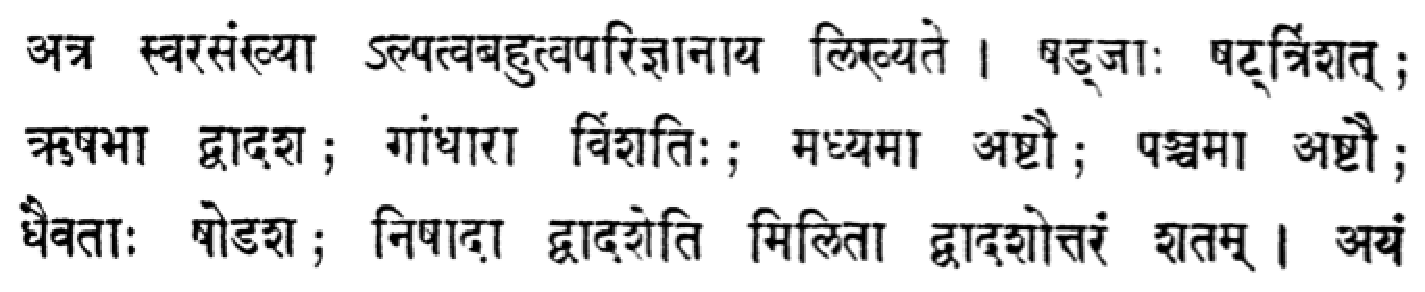
\includegraphics[scale=.35]{figures/5.eps}
\caption{Frequencies of \textsl{svara}-s in a particular \textsl{rāga}}\label{chap7-fig3}
\end{figure}
says (fig \ref{chap7-fig3}) “let us write down the infrequent or copious nature of the \textsl{svara}-s” in the \textsl{rāga} and lists \textsl{sa} as 36times, \textsl{ri} 12, \textsl{ga} 20, \textsl{ma} 8, \textsl{pa} 8, \textsl{dha} 16, \textsl{ni} 12, times out of a total of 112 \textsl{svara}-s. 

Given that Bhāskara had already written down multinomial theorem c.1150 C.E., it is not clear if anyone took the next step of using a device such as (informally at least) a multinomial distribution\endnote[51]{it models the probability of the total count after rolling a k-sided dice n times; here k is related to the number of different types of \textsl{svara}-s that can be used in a given raga and n the length of the non-\textsl{sāhitya} part under discussion.} to generate the svara-s as a first small step!

An even more sophisticated but related model is available in an outline from Ānandavardhana based on 
\begin{figure}[H]
\centering
\includegraphics{figures/6.eps}
\caption{Traces of \textsl{svara}-s of a \textsl{rāga}}\label{chap7-fig4}
\end{figure}

Bharatrhari’s insights. Here, \textsl{sphoṭa} is the suggester and \textsl{dhvani} the suggestion with \textsl{dhvani} elaborating \textsl{sphoṭa}. Using an aural point of view, \textsl{Sphoṭa} is said to arise from \textsl{sparsha} (contact), and produces a succession of sound waves, the \textsl{dhvani}, which is aurally perceptible. Just as there can be echoes for a well struck sound reaching us in a temporal sequence, there can be “echoes” of meaning at various levels, revealing the meaning sequentially. For example, Sreenivasa Rao says:

\begin{myquote}
The approach adopted by Bhartrhari in explaining the process of true cognition is significantly different from that of the other Schools. Bhartrhari argues that perception need not always be an ‘all–or-nothing process’. It could very well be a graded one. There could be vagueness initially; but, the perception could improve as one tries to gain clarity of the object. That is to say; the process of revelation could start from the indeterminate stage and progress, in steps, to the determinate stage. At each successive step, it gains increasing clarity. It begins from complete ignorance, passes through partial knowledge and ends up in a complete knowledge.

Thus, the position of Bhartrhari is that the overcoming of error is a perceptual process by progressing through degrees of positive approximations. Even invalid cognitions can sometimes lead to valid knowledge (say, as in trial-and-error). Initial errors or vagueness could gradually and positively be overcome by an increasingly clearer cognition of the word form or \textsl{Sphoṭa}. That is to say; the true cognition, established by direct perception, could take place, initially, through a series of possible errors; but, finally leading to the truth. (Rao dhvani)
\end{myquote}

Hence we can say that Bhartrhari is arguing for what is now called a “Bayesian model” for the evolution of “meaning”. In the initial stages, the meaning is the “prior” given by the \textsl{abhidhā} of the \textsl{pada}-s; as other information trickles in, the meaning changes with an associated probability distribution. The background, \textsl{kāla}, \textsl{deśa}, etc. of the hearer or the experiences (\textsl{anubhāva}) of the \textsl{sahṛdaya} decides the specific distribution finally used. 

A mathematical structure with a probabilistic generative model such as a “Latent Dirichlet Allocation” (LDA), also called “graphical models”, may be needed as a starting point (as it is only a “bag-of-words” model, and \textsl{ārohana and avarahona}, for example, cannot be handled directly) and interestingly research literature supports this view, at least in the \textsl{rāga} domain. Here, \textsl{svara}-s are like words, musical phrases (eg. \textsl{sanchāra}-s in Karnātic or \textsl{pakad-}s in Hindustāni music) like sentences, and \textsl{rāga}-s topics\endnote[52]{Extensions can be attempted, possibly with just a different set of constants in the generative models for some, but more details for others, for structures such as \textsl{pallavi, anu-pallavi, chiṭṭa-svaram, muktāyi-svaram,caraṇam,rāga-mālikā-}s, \textsl{kīrtana}-s, etc.}. Furthermore, each \textsl{gamaka} (ornamentation) can be seen to be a time series but distributed in a range of adjacent \textsl{svara}-s. Recent research in machine learning has shown how some context sensitive aspects can be attempted to be included in extended LDA-based models. In the case of \textsl{rasa} theory, a model would have to incorporate how \textsl{bhava}-s are characterized as \textsl{sthyāyī}, \textsl{sanchārī/vyabhicharī}, and \textsl{sāttvika} as well as how \textsl{ālambana}/\textsl{uddīpana vibhāva}-s produce the \textsl{bhāva}-s that finally become \textsl{anubhāva}-s. Given the extensive and detailed psychosomatic modelling in texts like \textsl{Nāṭyaśāstra}, it is not easy to come up good validated models that correspond to the insights therein. We however believe such a modelling perspective is possible, using some approximations, across many \textsl{kalā}-s using more detailed graphical models. Interestingly, in the domain of art and sculpture, VS Ramachandran and Hirstein have theorized about a “peak shift” for understanding the stylized portrayal of human (female) forms which, though anatomically difficult, are aesthetically pleasing (Ramachandran 1999); this may be seen, in a basic model, as a change in the constants in a generative model\endnote[53]{Furthermore, there could be a meaningful “quantum neural computing” model as (Kak 2008) has argued but we will not pursue it here.}.

A composer of an art form uses a sequence of atoms (\textsl{svara}-s, \textsl{mudra}-s, \textsl{gana}-s, etc) to express some \textsl{bhāva}/\textsl{rasa}. It is likely that, across art forms, only a few limited \textsl{bhāva}-s are available but with \textsl{sahṛdaya}-s it can be large. The mapping, too, is not completely definable (as per Bhartrhari’s paradoxes). The actor (or the director) has to understand what these sequences of atomic units mean or perceived to be, or it could even be indeterminate (just as with a series of \textsl{svara}-s). It is possible that there are multiple meanings and the actor has to emote a suitable one, or leave it open ended (as in the case of the meaning of \textsl{svara}-s in a musical phrase).

Now supposing that we understand the basic units of each art form, the next step is to help understand \textsl{bhāva}/\textsl{rasa} as a phenomenon in the context of a composer, an enactor and a \textsl{rasika}/audience. It is clear that there is some element of simulation (vide śankuka and keeping also views of other thinkers against this perspective); neurologically, the mirror neurons\endnote[54]{There are some nerve cells (“mirror neurons”) in the frontal lobes thought to be involved in the production of complex movements but which also fire when the animal perceives the same movements performed by an experimenter (Pellegrino1992).} are likely to be implicated. There seems to be also a large mirror neuronal complex that seems to be at work with respect to enactment and spectating. Just as in the attribute grammar formalism of synthesized and inherited attributes, neuronal outputs can be synthesized or inherited!

The second part is the communication itself through an actor, reader, music performer, etc. The theoretical questions here are whether these intermediaries experience the \textsl{rasa}s themselves! Whether these are real or virtual? Some of the questions are: does the enactor feel the \textsl{rasa} or only the \textsl{rasika}? Abhinavagupta argued for the former while later scholars such as Rūpa Goswāmi the latter. Again, from a neuroscience perspective, depending on the inhibitor circuits with respect to mirror neuronal complex, both seem in principle feasible (just as Bharata left both possibilities open).

The effect of some sequence of atomic units can be postulated as a combination of a cognitive state + affective state. Affective states are not cognitive, hence more likely related to non-representational aspects in the nervous system, especially evolved for quick involuntary responses such as “fight or flight” responses (mediated by the sympathetic nervous system) or “feed and breed” responses when body at rest (mediated by the parasympathetic nervous system) but these are whole-body responses (unlike “local” inflammations or infections). With respect to \textsl{rasa}, the parasympathetic system is likely to be more pertinent. To proceed further, we postulate a plausible neurobiological model here; our model is not dissimilar to more detailed models in neuroscience research literature (for example, Roger Orpwood’s theory discussed earlier). To aid in a quick emotional response, neurotransmitters (such as acetylcholine in the parasympathetic system) or other neuro-chemicals are generated by the nervous system that in turn is accepted by various types of receptors present in various organs such as the heart, stomach, etc, for producing an affective physical response. Since the number of such neuro-chemicals combinations are limited (contrast with the extremely large number of self and alien molecules to be recognized in the immunity system (in the billions) and the corresponding matching molecules to be produced), one can postulate that the \textsl{bhāva}-s generated, even if many, are most likely common across art forms. 

If only sub-critical sets or quantities of neurotransmitters/neurochemicals are produced, there will be no clearly identifiable state. If \textsl{bhāva}-s are sustained repeatedly (“\textsl{sthyāyi}”), a specific \textsl{rasa} will result (connections with Orpwood’s theory for qualia can be recalled here). Initially, the \textsl{rasa} response can be said to be very dependent on \textsl{vibhāva}-s, but if positive feedback loops are present, the response can become independent of the initial excitation. Depending on the specific components of the \textsl{bhāva}-s, different \textsl{rasa}-s may be possible. Furthermore, given the \textsl{anubhāva}-s in the model, we have a Bayesian model, possibly a mixture model.  

These \textsl{bhāva}-s, though in principle infinite in number as Bharata mentions, only a few “high level” \textsl{bhāva}-s are learnable in any cultural setting and this could be a differentiating marker across cultures. Interesting questions that arise are: Can we show that the \textsl{bhāva}-s produced in music the “same” as those produced in drama, poetry, etc., especially in a neuroscience perspective? That is, is the connectome excitation patterns the same across the brain?

Are all the art forms potent in producing all the \textsl{bhāva}-s? While this seems to be unlikely (for example, consider \textsl{tālavādyas} such as \textsl{mridaṅgam} or even simpler non-tonal ones), one can pose a Turing-like question: Is there a universality notion (ie. is the art form complete in some sense)? Similarly, is there a mapping, say, of some \textsl{svara}-s to \textsl{mudra}-s? We have already mentioned the mapping between colour and \textsl{bhāva}/emotions earlier in the \textsl{Viṣṇudharmottara} (and this phenomenon is also known through synaesthetes). Some studies have shown that a sudden transition from low to high pitch often indicates pathos across many cultures; however, while some gestures may be common across cultures, there may be some with possibly opposite semantics!

Another question is whether “\textsl{rasa}” is accessible to all? While there are many possible responses to this question, the Indic tradition affirms it with respect to \textsl{bhakti rasa}. Rūpa Goswāmi, in his development of \textsl{bhakti rasa}, says that enjoying \textsl{rasa nitya} is possible if one views life in terms of drama, using the language of \textsl{rasa} and redirecting it toward the development and expression of \textsl{bhakti}.

Going by our brief discussion of Bhartrhari’s paradox, it should be clear that the mapping from a specific enactment of an art form to the \textsl{rasa} in general is “non-computable”; ie. it is not clear a priori what output is to be expected for a particular event. This is where different civilizational impulses can be seen: \textsl{manodharma} in the Indic case but realism or carefully constructed “scores” that had to be reproduced precisely and accurately in the European one. 

\subsection{A computer systems model for communication across multiple roles and multiple persons}\label{chap7-sec4.2}

This section can be skipped by those who are not exposed to computer systems notions of virtual machines and the like. In computer science, we have the notion of a “virtual” machine that is emulated or simulated by a more “physical” machine, as there can be many levels at which this emulation or simulation notion can happen. The inputs and outputs of these virtual machines can be demultiplexed or multiplexed as necessary.

In an art form, there is the self of the spectator/reader (“3S”), the self of the composer/creator (“1S”) and the self of the enactor” (“2S”); the 1,2,3 refer to first person, 2nd person and 3rd person respectively with S standing for the self. Let us take a simpler case first. Crucially, the ability to empathise with someone depends on a person (“1S”) being able to imagine the state of someone else (“3S”); if there is considerable depth of feeling, there could be corresponding changes in the emotional state also. For this to happen, it is critical that both the self of the person (“1S”) and that of the sympathised (“3S”) be operative at the “same” time (or “timeshared” frequently enough, from a scheduling point of view). In a computational sense, one can imagine a type-II virtualization scheme where the “1S” machine, 1SM, runs a new virtual machine for the “3S” machine, 3SM, and sets it up in such a way that some of the inputs to 1SM, “seized” as necessary, are “tunnelled” to 3SM. The outputs of the 3SM virtual machine have to be carefully steered; if the outputs are “tunnelled” out of the 1SM then we have perfect isolation between 1SM and 3SM. But tunnelled out to whom or where? There could be some output devices “seized” by 3SM. In which case, the drivers of 1SM will be used for output to these devices. Or, alternatively, 3SM delegates the output function to 1SM system, and 1SM simulates the output function.

If this is not possible to answer, one solution is for the 1SM to directly indicate the output (ie. use 1SM’s drivers to communicate with the ext world). But this means that 1SM cannot indicate externally the state of 3SM. 

Some of the questions posed in the Indic tradition:
\begin{itemize}
\item[(i)] Can the enactor feel the \textsl{rasa}? If the outputs of the VM are tunnelled out or faithfully emulated, then the enactor (“2S”) need not sense anything. Otherwise, one can argue that there will be some “leakage” of the \textsl{rasa} into the enactor. Abhinavagupta argues for the first case. However, it is well known that leakage of state from one VM to another is possible due to non-virtualizable features (“sensitive instructions”) or due to non-isolation from a performance perspective. 

\item[(v)] Since we are dealing with a CPS, and the enactor (“2S”) has to signal the emotions through \textsl{mudra}-s and the like, the outputs of the 3SM have to be again transcoded and presented to the audience through the 1SM’s physical gestures. Here it can be \textsl{lokadharmi}\endnote[55]{\textsl{Lokadharmi} is realistic with a natural presentation of the world (similar to current movies) catering to the “common man”, whereas \textsl{nāṭyadharmi}, or stylized drama, uses gesture language and symbols, and more artistic but for \textsl{sahṛdaya}-s.} or \textsl{nāṭyadharmi}. The first one is suitable for a general audience but the latter most likely only for a \textsl{sahṛdaya}-s.

\item[(vi)] Should the identification of the enactor and the character be complete for “realism”? In the Indic tradition, the attempt is not so much at realism as to bring out the \textsl{rasa}. The attempt is more to trigger the desired cognitive/affective states in the \textsl{sahṛdaya}-s symbolically thru \textsl{mudra}-s and the like. Hence the gestures are stylized and the grammar of gestures generates the desired states.

\item[(vii)] Can the self be “unitary”? This problem is similar to the issues in the sleep states in the Indic tradition. Vedānta postulates a basal self across the sleep states to answer the question why we “know” that we slept deeply but at the same time we “did not know anything” during that time. Here, we have multiple VMs and therefore the basal self (or the “host OS”) is responsible for switching between various emotions or even across multiple characters.
\end{itemize}

There is also an interesting problem in the context of a CPS + \textsl{rasa}: do we need in general a self-reproducing machine? Note that each emulated living entity will have a corporeal aspect that has to be used to communicate interactions with the real world; this means, the simulated VM needs to have a physical body too (for eg, an elephant, bird, \textsl{devi}, etc) and realized at run time. In the most general case, given the person/living entity to be conveyed, we need the physical emulation/realization using the body of the enactor. For ease, many \textsl{mudra}-s have been instead developed to represent the various entities (eg. parrots).

\subsection{Rasa in Music: an example}\label{chap7-sec4.3}

Let us consider music first. We first discuss the cognitive part. In the earliest phase, Vedic chanting in Sāma Veda used 3 \textsl{svara}-s and it was extended later in music to 5, 7, 12, 22, ... \textsl{svara}-s; these numbers Kak points out may be related to Meru prastāra. There were obviously deep connections with \textsl{chandas}/poetry and redundancy/checksums as anti-entropy measures with various styles of chanting such as \textsl{pada}, \textsl{krama}, \textsl{jaṭa}, \textsl{māla, śikha, rekha, dhvaja, danda, ratha, ghana}. Phonological combinations (\textsl{sandhi}) have been devised taking into account what is realizable given our human anatomy with respect to speech; they result in lesser effort and so can be said to be euphonic. If iterative or recursive structures are devised, “vibrational” sensations can in principle be auditorily excited. Historically, for example, Mataṅga discusses \textsl{Ṣadja}-\textsl{grama} and \textsl{Madhyama-grama} as two basic \textsl{Grama}-s (groups or clusters); \textsl{grāma}-s are collection of \textsl{svara}-s in consecutive order. From these arise \textsl{Mūrchchanā}, \textsl{Tāna}, \textsl{Jāti} and \textsl{Rāga}. \textsl{Mūrchāna}-s are a set of systematic rotations of the \textsl{saptaka} with an \textsl{ārohana} and \textsl{avarohana} (so 7 for each \textsl{grāma}). These are described by Bharata earlier also but something deeper in structure was felt to be needed; this sense later resulted in the innovation of the \textsl{rāga} paradigm\endnote[56]{We can take as an example a \textsl{rāga} that falls in the "\textsl{adbhutarasa}" (wonderment and awe) of the \textsl{navarasa-}s (nine emotions). \textsl{Kumudakriyā}, the \textsl{janya rāga} of \textsl{Pantuvarāli (Kāmavardhinī)}, 51st \textsl{melakartha} has been chosen by Muthuswami Dikshithar for his composition, “\textsl{Ardhanareeswaram}”. See \url{https://www.youtube.com/watch?v=b5yuBGJugFw} (Kuldeep Pai) or \url{https://www.youtube.com/watch?v=E1HA1XPFT-M} (Aruna Sairam). The scale of \textsl{Kumudakriyā}-Ascending is Sa Ri Ga Ma Dha Sa with descending being Sa Ni Dha Ma Ga Ri Sa... A \textsl{rasika} comments “Contemplation on the \textsl{prayoga}-s or phrases Sa Ni Dha Ri', Ri Ga Ma Dha Ri, etc. invoke a sense of fantasy, make-believe or illusion. Imagine suddenly walking into somebody who is split into a perfect half of a perfect man and a perfect woman! ... Absolutely dazzling and surreal! \textsl{Kumudakriyā}, a breathtaking raga of fantasy, ...”}. From iterative structures, the musical ideas turned to probabilistic ones\endnote[57]{See also, for eg. (Rowell 1992), for a comparable explanation: “What does this tell us about the relationship between theory and practice? A hallmark of the early Indian way of thinking about music was to identify and name all possible permutations of the basic elements, but with the realization that only certain authorized (and far more specific) melodic constructions can become the basis for actualized music, as, for example, in the form of an individual raga. It was the job of theory to provide the widest selection of possibilities, but it remained for practice to select the most pleasing of these arrangements. There is a reason for this: any purely mechanical set of permutations of a given system (of which the diatonic scale is an excellent example) will sooner or later exhaust the available possibilities and will admit no others. Such an outcome would violate a basic assumption of Indian culture, namely, that the number of available forms is, at least in theory, unlimited. The solution, which is as valid today as it was two thousand years ago, was to achieve the richness and profusion of forms that Indians demanded in their music by means of a musical system that could not be confined to any set of exclusive possibilities. On the contrary, they sought to devise a system that could accommodate any number of later additions, a system that was inclusive rather than exclusive. What the \textsl{mūrcchana}-s and their derivatives provided was the simple notion that different octave segments (the \textsl{mūrcchana}-s) and certain of their subsets (the \textsl{tana}-s) could when colored by the emphasis or understatement of certain tones, and also by distinctive ornaments and melodic pathways- form the structural basis for a unique melodic construction: a \textsl{jāti}, a \textsl{grāmaraga}, or a \textsl{raga}.”}.

A simplistic description for a \textsl{Rāga} is as follows: choose an alphabet of \textsl{svara}-s, use well established \textsl{sanchāra}-s or \textsl{prayoga}-s (“signatures”) of the \textsl{rāga}, and follow rules of \textsl{ārohana} and \textsl{avarohana} to generate yet more possible strings of \textsl{svara}-s as music. In actuality, there are many more critical features such as \textsl{amsa} (prominent or \textsl{jīva svara}-s), \textsl{alpatva} (\textsl{svara}-s that need to be present fewer in number), \textsl{bahulatva} (copious), \textsl{ṣādava}/\textsl{audava}: 6 note/5 note \textsl{sanchāra}-s, \textsl{antara mārga}: the introduction of note or \textsl{chāya} of another \textsl{rāga}. Furthermore, only when the "\textsl{jīva svara}-s” are rightly used, we can induce life into a \textsl{rāga}.

RN Iyengar has suggested that a rāga is actually a svara time series, evolving in the space of ārohana-avarohana (scale) with the property of ‘alpatva-bahulatva’ (Iyengar 2017). Furthermore, “The scale can be nearly equated with the sample space of Probability Theory”. He also points out that Sārngadeva actually gives many traces (sequences) of \textsl{svara}-s for one \textsl{rāga} as an illustration; this has been discussed earlier.

Fundamentally, a \textsl{rāga} is not a static concept (due to notion of \textsl{manodharma sangīta}) and has a stochastic aspect. Iyengar and others have pointed out that the time series of \textsl{svara}-s can be modelled as a AR(1) process (AR: autoregressive (stochastic) process) with the following 1st order simple model: $\Phi(n) = k*\Phi(n-1)+$ noise, where $\Phi(n)$ is the \textsl{svara} at time unit $n$ and $k$ is a constant; many simple songs taught to beginners (“\textsl{pillāri gītam-}s”) have been shown to have this AR(1) property! More complex songs need many more terms as a AR(p) process that depends not only on on the $(n-1)$ instant, but on $(n-2),\ldots (n-p)$ instants. These can be shown experimentally by computing autocorrelation functions (ACF).

Furthermore, Iyengar says that the ACF of a \textsl{varnam} has a fractal-like structure and he conjectures that \textsl{kīrtanams} in any \textsl{rāga} will be a more complex time series, exhibiting finer self similar structures embedded in the sample space. He posits that \textsl{rāga ālāpana} is actually a chaotic process with the \textsl{ārohana}-\textsl{avarohana} providing the boundary of the “strange attractor”. As all of this is heard and experienced, \textsl{rāga} can be said to be a mathematically based stochastic process that generates \textsl{rasa}!

In addition, using machine learning algorithms that use generative models (such as “LDA”), some researchers have shown higher rates of correct classification of \textsl{rāga}-s. (Of course, other models like “profile” HMMs (pHMM) could also be profitably explored; a pHMM has a profile that could apply to the parent raga with janya rāgas being generated using the pHMM structures). These also imply deep down that a \textsl{rāga} has a substantial and inescapable stochastic structure that also can be discerned but which is sufficiently mathematically tractable. This is historically interesting: almost one millennium earlier, there has been the groundbreaking generative model of Pāṇini in his \textsl{Aṣṭhādhyāyi} except that stochastic processes do not play a role in his system and his grammar is closer to a term writing system such as the Post Correspondence system formalized mathematically in 1920’s. For \textsl{rāga}-s, we also have a generative system but with a probabilistic core!

Next to briefly discuss the affective aspect of Indic music, the word \textsl{rāga} itself is defined as “\textsl{ranjayati iti rāga}”. There has been attempts at theorization at 2 levels of structure: at the level of \textsl{svara}-s and at the level of \textsl{rāga}-s themselves. \textsl{Viṣṇudharmottara} (III.18, 2-3, tr. Priyabala Shah) gives the following scheme: “for hāsya and \textsl{śṛṅgāra, madhyama and pancama} are used; for \textsl{vīra, rauḍra} and \textsl{adbhuta, śaḍja} and \textsl{ṛṣabha} are used; for \textsl{karuṇa, niṣāda} and \textsl{gāndhāra} are used; for \textsl{bībhatsa} and \textsl{bhayānaka, dhaivat} is used and for \textsl{śānta, madhyama} is used. Similarly for different \textsl{rasas} different \textsl{layas} are used.” Some theorists assign \textsl{rasa} or \textsl{bhāva} to \textsl{rāga}-s on the basis of their \textsl{vādī} (dominant note) in the following way: infinity or space if the \textsl{vādī} is \textsl{sa}; illumination if the \textsl{vādī} is \textsl{re}; devotion if the \textsl{vādī} is \textsl{ga}; erotic if the \textsl{vādī} is \textsl{ma}; joy or contentment if the \textsl{vādī} is \textsl{pa}; valour and disgust if the \textsl{vādī} is \textsl{dha}; and encouragement if the \textsl{vādī} is \textsl{ni}\endnote[58]{Discussed interestingly in the CBSE class XI Music text (CBSE 2012).}. Alternatively, \textsl{pa} (\textsl{panchama}) is said to be for \textsl{śṛṅgāra}; for example, \textsl{Gita Govinda} 1.39 refers to a song being sung in \textsl{panchama rāga} to evoke \textsl{śṛṅgāra}.

There is a long tradition in assigning \textsl{rāga}-s for evoking emotions in \textsl{Hindustāni} and \textsl{Karnātic} systems. For example, \textsl{Śubhapantuvarāli} is said to indicate penitential emotions whereas \textsl{Athāna} that of \textsl{vīra rasa} and so on. Starting with probabilistic emphasis on the \textsl{vādi} notes, specific \textsl{rāga}-s also indicate the emotions using musical phrases observing \textsl{ārohana} and \textsl{avarohana}, with specific phrases (the \textsl{sanchāra}-s/\textsl{pakad}-s in Karnātic/Hindustāni music, for example) being the signatures. Since there is no written score, each phrase can be elaborated multiple times possibly with different ornamentation; there is thus probabilistic emphasis on different phrases as well as ornamentation (“\textsl{gamaka}”) giving rise to a richly textured music that can evoke deep emotions. Even \textsl{tāla}-s are expected to contribute to the \textsl{rasa}; for example, \textsl{pratimantha tāla} is said to enhance \textsl{śringāra} (Narayanan 2016). 

The Indic seers (take, for example, Abhinavagupta) intuited music’s capacity to help us to approach the transcendental plane and this has been borne by recent studies; for example, Janata and others, as discussed before, have identified the temporo-parietal junction (TPJ) region that is the location of self-referential activity is the locus of music also. Music is a highly personal experience while making us also feel a part of the whole “universe” in an abstract way; interestingly, the notion of \textsl{sādhāranikaraṇa} is useful in the latter as it posits universals across all.

\section{Computational Thinking and its relevance for \textsl{Rasa}}\label{chap7-sec5}

While one running thread in Indian aesthetics or \textsl{rasa} is the taxonomical approach, it was married, often enough, to a computational base. While the taxonomy part has been widely recognized (for example, the \textsl{vyabhicāri-bhāva}, the transitory state of mind or body, said to be 34 in number such as \textsl{asūyā, nirveda, glāni, śaṅkā} etc), the computational aspect has not been appreciated as much and one can say that this served possibly as a possibly unique or distinguishing part of the tradition. Furthermore, detailed psycho-physical (taxonomical) models in, for example, \textsl{Nāṭyaśāstra} are helpful in a computational model as we have discussed in Section 4 for modelling emotions. We now give some examples of computational thinking and its relevance for \textsl{rasa} in a few art forms, mostly from a generative perspective; the interested reader can find some background on computational thinking and the specific Indic context as two appendices (APPENDIX 1 and 2). Note that when we discuss \textsl{rasa} here it is at a more general level and not only in the context of Bharata’s formulation.

\subsection{The Computational Basis of \textsl{Rasa} in Poetry}\label{chap7-sec5.1}

The Vedas are alternately called as “\textsl{chandas}", thus there is close connection between poetry and visions of reality (“\textsl{rtam}”). The study of poetry therefore assumed an important part of the intellectual tradition, for example, \textsl{nirukta}, \textsl{śikṣā}, etc. Continuing in this tradition, Pingala enumerated the number of \textsl{tāla}-s through cryptic sutras in \textsl{Chandaḥśāstra}. The motivation doubtless was that if we need to understand music, it helps to know, if feasible, how many possibilities exist for a specific entity in a system that need to be examined individually for tractability or practicalness\endnote[59]{See (Rowell 1992) for a comparable explanation.}. The idea here may have been to possibly look at all possible ways of structuring syllables, long or short, given a specified amount of time and in the process invented Pingala sequence (P), now inadvertently called Fibonacci series (0,1,1,2,3,5,8,13,...)\endnote[60]{Fibonacci wrote a book, about 1202, that discussed Indian mathematics, translated into Syriac/Arabic, as the basis; the name for the series was given only in c. 1870's by Lucas who proved \verb|2^{127}-1| is prime using these numbers.}. Pingala or his disciples also noted that in this sequence the next term is given by the sum of the 2 earlier terms (starting from the 3rd term). Elaborating explicitly (Knuth 1997), Gopāla (before 1135 C.E.) and Hemachandra (around 1150 C.E.) give the number of \textsl{tāla} (rhythmic patterns) for \textsl{M mātrā} (beats) (“P(\textsl{M})”) with \textsl{anudruta} (1-beat) and \textsl{druta} (2-beat) algorithmically as \textsl{tāla} (\textsl{M}) = \textsl{tāla} (\textsl{M}-1) + \textsl{tāla} (\textsl{M}-2), or P(\textsl{M}) = P(\textsl{M} -1) + P(\textsl{M} -2)\endnote[61]{The recursive or iterative property of the series can be seen as follows by case analysis, as either an \textsl{anudruta} comes first or the \textsl{druta}. First fix a \textsl{anudruta} as the 1st in the sequence; the remaining (\textsl{M}-1) beats have P(\textsl{M}-1) distinct possibilities. Next, fix a \textsl{druta} as the 1st in the sequence; the remaining (\textsl{M}-2) beats have P(\textsl{M}-2) distinct possibilities. The sum therefore gives P(\textsl{M}).}.

Investigating \textsl{chandas} further, the concept of \textsl{gana}-s were introduced. These are groups of 3 syllables, \textsl{anudruta}/short/\textsl{laghu} (“U”) or \textsl{druta}/long/\textsl{guru} (“|”); hence 8 possible \textsl{gana}-s (inaugurating the start of binary notation, now commonplace). From a coding perspective, each specific \textsl{gana} can be considered as the “summary” or checksum/hash of 3 syllables\endnote[62]{Interestingly, the process of coming up with a mnemonic for remembering the various \textsl{gaṇa}-s (“\textsl{yamātārājabhānasalagam}”) threw up the earliest known example of what has later been called memory wheels (first noted in 1880’s by those working on codes in telegraphy) or de Bruijn sequences (1944) (see (Knuth 2011)).} and hence the sequences of these summaries can be used as a way to detect corruption if the poetic structure is violated. These are described in \textsl{alaṅkāra śāstra}-s, for example, the \textsl{śārdulavikrīdita} with “msjsttg” structure, redolent of the forest as it recalls a tiger cub’s playfulness (with \textsl{virāma} in the 12th syllable and then another 7 syllables away). Since \textsl{alaṅkāra śāstra} and its connection with \textsl{rasa} has been discussed in the tradition widely, we focus on other aspects, specifically the computational as it relates to \textsl{rasa}. The choice of meters widely used could be connected with the locality principle we discussed in the context of music; the locality could be in terms of pitches\endnote[63]{In Telugu, \textsl{prāsa}is also present to a considerable degree: for example, use of same consonant at fixed positions.} as the poem is recited or in terms of sequenced “chords” of \textsl{gana}-s (but different from W Music chords!)

Because \textsl{rasa} is now married to function, there is a robustness in the transmission of \textsl{śloka}-s written to various types of \textsl{chandas} that is not possible in other traditions except in a rudimentary way. Advancing the robustness further, in the Vedic domain, the generative aspect interestingly has been further married to a functional notion, that of resistance to local decay or destruction (reliability in short) either when chanted orally or when written on fragile materials; this again depends on a computational basis. Chanting styles (\textsl{vikratis}) were invented that introduced controlled amounts of redundancy such as \textsl{krama, jaṭa, māla, śikha, rekha, dhvaja, danda, ratha, ghana}, with the \textsl{ghana} being the most complex (the sequence of syllables a1 a2 a3 a4, for example, being chanted, 3 syllables at a time but sliding with one syllable at a time, as a1 a2, a2 a1, a1 a2 a3, a3 a2 a1, a1 a2 a3; a2 a3, a3 a2, a2 a3 a4, a4 a3 a2, a2 a3 a4, an expansion by a factor of 11 with a corresponding increase in robustness with respect to local decay). The repetition in these codes has a hypnotic effect when chanted as those who have heard \textsl{ghana pāṭha} can testify. The Indic imagination therefore approvingly quotes \textsl{āśrama}-s and such where such recitations would continue “nonstop”.

Kashyap and Bell have investigated the robustness of such chanting styles using coding theory and formulate \textsl{Krama-māla} style of chanting as a “rate 1/4 linear block code over a finite Galois field”; they show that with this code a text of 4n symbols can be corrected even with as many as 2(n-1) errors under some assumptions (Kashyap 1998). While requiring the preservation of the order of words, the errors to be detected are the add/delete of a syllable/word in a word/sentence or avoiding “long jumps”. To explain the latter, consider a set of syllables A (in verse x) that is similar to a set B (in verse y) and we are chanting of  ...AC... ; ...BD... Now we can mistakenly chant say ...AD... or ...BC..., ie “jump” across due to similarity between A and B. Specific styles of chanting such as \textsl{avichakra} \textsl{ratha} handle these by appropriate coding. Kashyap and Bell give the following interesting example as it involves the very first mantra in RV:

\begin{myquote}
RV 1.1.1     ... C ratnadhātamam (A)

RV 1.20.1    ... E ratnadhātamaḥ (B) D
\end{myquote}

Chanting is coded so that A chained to C and B to E to prevent jump from C to B and E to A. If there is incorrect chanting, this code can point out the error. 

Using such computational coding ideas, Vedas have been transmitted mostly orally across at least 3500-5000 years without differing versions including exact pronunciation (with, it is said, only one doubtful reading in Rigveda at RV7.44.3 after a lapse of as much as 7000 years)! UNESCO proclaimed the tradition of Vedic chant a “Masterpiece of the Oral and Intangible Heritage of Humanity” on November 7, 2003. (Of course, such clever mathematical ideas cannot survive wholesale destructions of cultures that spawn them as happened with the Indic ones, especially in Kāśmīr.)

Continuing in the same strain, surprise or wonder as a generative component of \textsl{rasa} could be channelled computationally for linguistic problems that need techniques such as backtracking; for eg. knight’s tour problem considered by Rudraṭa and also by Vedānta Deśika and many others. The earliest known reference to the knight's tour problem dates back to the 9th century C.E. by Rudrata\endnote[64]{after a correction as the \textsl{śloka}is given wrongly; Wikipedia article on “Knight’s Tour” accessed Jan 10, 2016}:

\begin{myquote}
“In Rudraṭa's \textsl{Kavyālaṅkāra}[3] (5.15), a Sanskrit work on Poetics, the pattern of a knight's tour on a half-board has been presented as an elaborate poetic figure ("\textsl{citra}-\textsl{alaṅkāra}") called the "\textsl{turagapadabandha}" or 'arrangement in the steps of a horse.' The same verse in four lines of eight syllables each can be read from left to right or by following the path of the knight on tour. Since the Indic writing systems used for Sanskrit are syllabic, each syllable can be thought of as representing a square on a chess board. Rudraṭa's example on a 4x8 “board” is as follows:

senā līlīlīnā nālī

\qquad līnānā nānālīlīlī |

\qquad nālīnālīlī nālīnā

\qquad līlīlī nānānā nālī ||
\end{myquote}

For example, the first line can be read from left to right or by moving from the first square to second line, third syllable (2.3) and then to 1.5 to 2.7 to 4.8 to 3.6 to 4.4 to 3.2.” (Knight 2018) 

Rudraṭa has simplified the complexity of the puzzle by adopting only 4 syllables and this also leads to the interesting result of knight’s move verse being the same as the original verse\endnote[65]{Namisadhu, the commentator, after explaining the meaning of the verse, gives a cryptic mnemonic verse in his commentary which reads as follows:
\begin{quote}
\textsl{kaśakhenāgabhaṭāya tathakeveñarāghave} |\\
\textsl{ṣajethāḍhepacemeṭhe doṇasachalaḍephaṅe} ||
\end{quote}
The above verse gives the knight’s moves if numbers are attached to the consonants as they appear in the \textsl{varnamāla} (see table below from G S S Murthy \url{murthygss@gmail.com}):
\begin{figure}[H]
\centering
\includegraphics{figures/9.eps}
\end{figure}}. Note that finding whether a knight’s tour exists, without worrying about a poem as part of the jumps, is itself a non-trivial combinatorial problem and uses what is called the backtracking technique in computer programming. The problem considered by Rudraṭa\endnote[66]{Interestingly, Rudraṭa’s thinking was a bit ahead of his times, as Dasgupta, Papadimitriou, Vazirani discuss in their book on “Algorithms” 2006, a graduate-level CS text by experts in the field: “Almost a millennium before Euler’s fateful summer in East Prussia, a Kashmiri poet named Rudraṭa had asked this question: Can one visit all the squares of the chessboard, without repeating any square, in one long walk that ends at the starting square and at each step makes a legal knight move? ... Let us define the RUDRAṬA CYCLE search problem to be the following: given a graph, find a cycle that visits each vertex exactly once---or report that no such cycle exists. In the literature this problem is known as the Hamilton cycle problem, after the great Irish mathematician who rediscovered it in the 19th century. Define the RUDRAṬA PATH problem to be just like RUDRAṬA CYCLE, except that the goal is now to find a path that goes through each vertex exactly once.” (Both problems are equivalent in terms of complexity as the Rudraṭa cycle problem is equivalent to the path problem or what is known in computer science as the Travelling Salesman Problem or TSP.). This text can be considered as a trend-setter in that, for this specific case, all traditional usage of the word Hamiltonian cycles or paths are eschewed and instead Rudraṭa cycles and paths are used. But they have not been consistent; for example, the Fibonacci series is called as such instead of Pingala or Gopāla series...}, Vedānta Deśika and many others in the Indic tradition is much harder as the knight’s tour should also produce a poem in addition. Vedānta Deśika had at least two such instances ($4\times 8$ “board”) in his \textsl{Pādukā-sahasram}, supposedly composed “in one \textsl{yāma} of a night” (ie. one fourth of a night) as part of a challenge. Many examples of \textsl{Citrakāvya}-s abound not only in Sanskrit but also in languages such as Telugu.

Note that Leonhard Euler was one of the first European mathematicians to investigate the (simpler) knight’s tour was but for the 8x8 board with H. C. von Warnsdorf in 1823 giving the first procedure for completing the Knight's Tour.

The theory of \textsl{Śleṣa} was developed extensively too, in ways that is difficult in other cultural and linguistic systems (see (Bonner 2010)). We do not discuss this further as its computational aspects are not clear or formalizable as of now.

What is remarkable is that going in depth to understand the wellsprings of poetry or \textsl{chandas} revealed to the Indic people a surprising combinatorial or algorithmic base and the whole world benefitted from these deep insights in combinatorics. But the Indic people’s creativity was mostly cut short post 1200 C.E. while other cultures benefitted from the transmissions of these ideas from India.

\subsection{The Computational Basis of \textsl{Rasa} in Music}\label{chap7-sec5.2}

Next we move to music; this will be discussed in brief as many of these aspects have been discussed or are reasonably well known. First there is the notion of \textsl{svara} and that of \textsl{śṛuti}. While the notion of interval, octave and fixed frequency seem to have been central in (later) Western music, the \textsl{svara} seems to be a realized sound on the background of a “fluid” set of \textsl{śṛutis} with all of these only relative. The the notion of 3, 7, 22 \textsl{svara}-s is argued by Subhash Kak to be based plausibly on mathematical principles (Kak 2004), as the numbers 3,7,12, 22 are important in Indic music and arise as a result of various \textsl{Meru prasthāna}-s that generate these numbers\endnote[67]{Prasthāna-s being either additive: $A(n)=A(n-1)+A(n-2)+A(n-3)$ or multiplicative: $M(n)=M(n-1)*M(n-2)+1$}. The 7 and 22 \textsl{svara} system is pre-\textsl{Naṭyaśāstra} (before 400 C.E.). Vinod Vidwans argues further that Bharata has an interesting (but little understood) generative metamodel which has but only a few rules for specifying \textsl{vādi}, \textsl{samvādi, vivādi svara-}s given a \textsl{svara} (Vidwans 2016). However, the mathematical closure of these rules gives all the 22 \textsl{svara}-s (\textsl{śruti}-s) in the system; this is part of his \textsl{śruti}-\textsl{nidarśanam} (“demonstrating microtones”). Venkatamakhin gives a systematic classification of \textsl{Melakarta raga}-s based on \textsl{svara}-s. In the fig \ref{chap7-fig5} below\endnote[68]{From wikimedia (credits to Basavarajtalwar, 4 Nov 2009)}, 2 types of \textsl{ma} (left half and right half), 2 types of \textsl{ri} and 3 types of \textsl{ga} (12 sectors overall), 6 combinations of \textsl{da} and \textsl{ni} (each sector) give rise to $2*2*3*6=72$ \textsl{melakarta}-s. This became widely accepted in the Karnātic tradition but a more intuitive model was retained in the Hindustani system. This system is not only based on simple combinatorics but also uses ingenious encoding of the names of the ragas itself to reveal its cardinal number in the \textsl{melakarta} scheme using \textsl{kaṭapayādi} encoding; we do not give details here due to lack of space.
\begin{figure}[H]
\centering
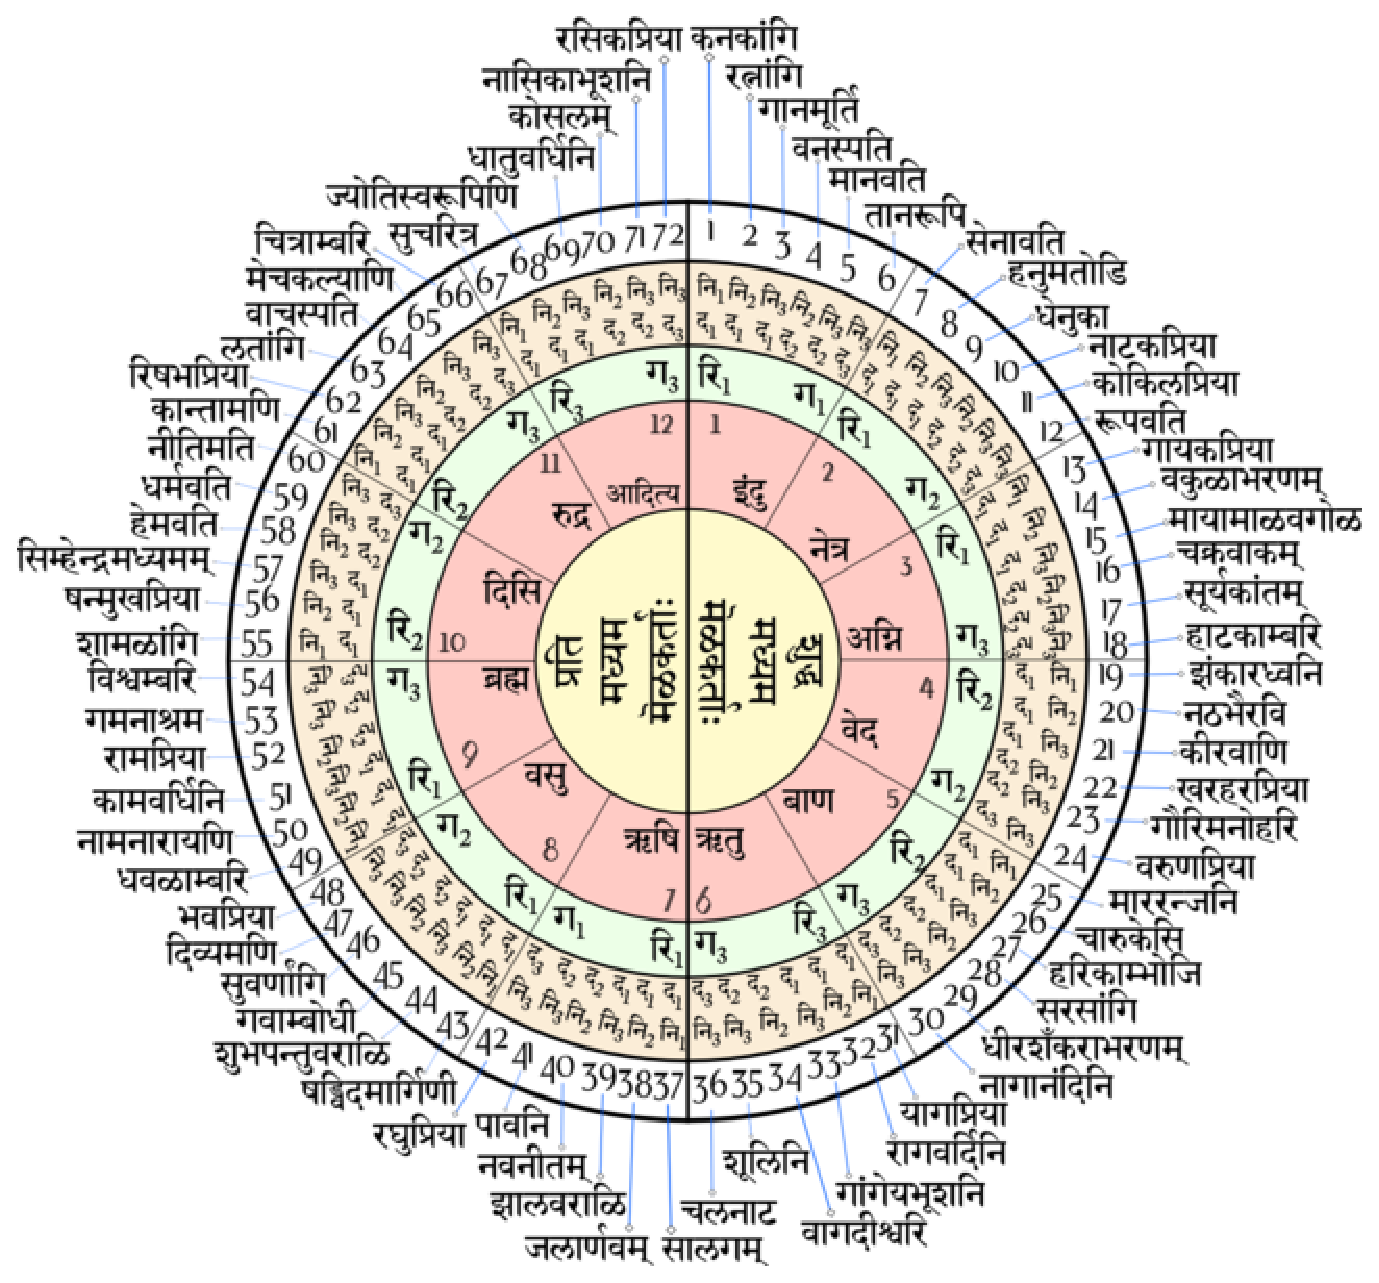
\includegraphics[scale=.4]{figures/7.eps}
\caption{Venkatamakhi’s Melakarta scheme (from wikimedia with credits to Basavarajtalwar, 4 Nov 2009)}\label{chap7-fig5}
\end{figure}

Next we briefly discuss \textsl{tāla} which is widely known to have a mathematical content. In the distinctive style of percussion instruments such as mridaṅgam, we have \textsl{korapu} or \textsl{yati}-s where phrases/duration have to be in arithmetic progression (increasing or decreasing). In addition, simple “diophantine” (another misnomer!) equations need to be solved to check feasibility of some \textsl{yati}. For example, there is a notion of \textsl{gati} that fixes how many syllables can go into a time unit of \textsl{tāla}. This notion is independent of the specific \textsl{tāla} itself. While \textsl{caturaśra gati} (4) is usually common, one can also attempt \textsl{triśra gati} (3), \textsl{khanda gati} (5), etc. Now if one is playing a iterative structure with a \textsl{yati} also woven in but now with a \textsl{triśra} instead of \textsl{caturaśra}, feasibility of this fitting into a given set of time units depends on solving some integer linear equation; if there is no solution, one has to creatively modify the structures by adding \textsl{virāma}-s or \textsl{edupu}-s (silent time units) to balance the equation but without destroying the aesthetic sense. Often multiple solutions are possible and they provide the variety seen. Some are quite tricky: for example, \textsl{sampūrna khanda nade} has 10 \textsl{akṣara}-s/8 units of \textsl{tāla}.

For a simpler example, consider 16 time units for a regular \textsl{tāla} like \textsl{ādi tāla}. If \textsl{caturaśra gati} is used, each \textsl{akṣara} could be 1/4th of a time unit. If a \textsl{moharā} or \textsl{muktāyi} (both are reasonably complex pieces 

that are repeated 3 times to exactly match multiple complete durations of a cycle of tāla (“\textsl{āvartana}”)) is now attempted to be played in a different \textsl{gati} (say, \textsl{tiśra} where each \textsl{akṣara} is now 1/3rd of a time unit), some tālas need adjustments; note that due to the “vernier” principle, the time keeping has to be sufficiently exact otherwise, unresolved differences of ⅓-¼ time units (1/12th time unit) or its multiples will wreck the experience. In the most difficult case, 1/7 - 1/9 = 2/63 time unit accuracy is needed!

There are many talas (such as \textsl{Dhruva, Maṭhya, Jhampa, Aṭa, Eka}) and many variations with respect to time units and also \textsl{gati}. It is difficult to remember the many sequences but experienced musicians remember high level patterns but calculate some details on the fly! If they do not have sufficient time to calculate, then they play known simpler patterns till they can calculate the details right! A similar system obtains in the Hindustāni (northern) system where for example tabla is used; it is not uncommon to see somewhat unusual beats of 10 and half being played for half an hour! 

"\textsl{Pancavādyam}" a traditional temple art instrumental ensemble (\textsl{timila, maddalam, ilathalam} and \textsl{idakka} - percussion; \textsl{kombu} - wind instrument) of Kerala. The performance is led by the \textsl{timila} and the “sense of sacred” is generated by the pyramid-like rhythm structure with a constantly increasing empo coupled with a proportional decrease in the number of beats in cycles.

\subsection*{The Computational Basis of \textsl{Rasa} Architecture}\label{chap7-sec5.3}

\begin{figure}[H]
\centering
\includegraphics[scale=.8]{figures/8.eps}
\caption{Rangoli pattern drawn by an artiste}\label{chap7-fig6}
\end{figure}

Starting from the earliest times (5000 years and earlier?), the sense of sacred was attempted to be given by geometry. The \textsl{śyena} geometry and its construction in the Vedic rites is a good example. Due to such examples and internal consistencies, A. Seidenberg argues for precedence of Vedic thought over Babylonians with respect to geometry (Seidenberg 1978).

Once recursive structure of language (Pāṇini) and number system has been mastered, it is an easy step to think of term rewriting rules (aXb$\to$pYq) or of mathematical series given by some (arithmetic/geometric) progression. The Indic thinking (Hindu, Buddhist, Jaina), having gone past the stage of building perishable structures, started experimenting with stone to build long standing structures. For example, the superstructures of \textsl{Nāgara} temples have a distinctive curvilinear form composed of a series of motifs with the surface geometry resulting from intricate mathematical and geometric expression based on stereotomic techniques (Kramrisch 1946), (Meister 1979).  A computational style thinking in such architectural ventures seems to have been common by 7-8 century C.E. already as we see in the majestic Ellora\endnote[69]{“From The {\sl\bfseries Alas} inscription dated 770 C.E. tells us that the Kailasanath temple was commissioned in 757 AD (or 773 AD) by {\bf Krishna I}, an uncle of the founder of the {\bf Rashtrakuta} dynasty, {\bf Dantidurga}. The construction work took about 150 years to complete. ... While the entire temple complex looks like it is a cluster of temples and pillars and sprawling halls, it was actually {\bf carved out by {\sl vertically} excavating some 200,000 tonnes} (or 400,000 tonnes according to others) {\bf out of a {\sl single}, mammoth rock}. It cannot be emphasized enough that the real achievement is that the entire temple complex was {\sl excavated, not constructed}. Indeed, it does evoke a sense of awe when we try and fathom what it must have taken in terms of mathematics, engineering, building technology, craftsmanship, artistry, design, planning, and the entire project execution when we recall that this “project” was executed over 150 years and spanned at least six generations of experts in all of these fields.” Indiafacts \url{http://www.indiafacts.co.in/ajanta-ellora-grandeur-cultural-amnesia-part-1} (accessed Jul 27, 2017)}; it seems to have reached its peak by 12 century C.E. (for example, Kandāriya temple in Khajurāho). 

Trivedi discusses the use of recursive structures in Indic (especially Hindu/Jain) temples to depict an “evolving cosmos of growing complexity, which is self-replicating, self-generating, self-similar and dynamic” (Trivedi 1989). Furthermore, “the procedures are recursive and generate visually complex shapes from simple initial shapes through successive application of production rules that are similar to rules for generating fractals.” The techniques identified are 
\begin{itemize}
\item[(i)] fractalization. A very simple example is going from n sides for a pillar to 2n sides next and repeat till we approach the shape of a circle; this can be seen in many temples where pillars with 4, 8, 16 sides and circles can be seen in the same enclosure. Similarly, Koch-like fractals are generated but on initial shapes more complex than a simple line. For example, for Koch fractal, the shape -------- is first transformed to ----/$\backslash$---- and each small segment is similarly transformed; if this procedure is repeated, the resulting shape is similar to the plans of some Hindu temples that display the “snowflake curves characteristic of fractal figures” (see figs. 2 and 3 in (Trivedi 1989)). The architectural texts discuss these techniques explicitly and also develop a vocabulary to describe the process (see fig. 17 in (Trivedi 1989)). The self-iteration can be \textsl{dvi-aṅga} (adding 2 more segments \textsl{karṇa} and \textsl{bhadra} where 1 existed), \textsl{tri-aṅga} (adding one more segment \textsl{pratiratha} to the \textsl{dvi-aṅga}), \textsl{caturaṅga} (adding segment \textsl{nandika} to \textsl{tri-aṅga}), \textsl{pañcāṅga} (adding \textsl{konika}), etc. 

\item[(ii)] self-similar iteration in a decreasing scale. Sambit Datta, discussing the geometry of temples, says “The surface of the superstructure is composed of a series of carved motifs that exhibit a progressively diminishing sequence of self-similar forms. While no guide exists in the canonical literature on how these sequences are handled, two clues are available in the mathematical and cosmological texts. First, the notion of \textsl{śūnyatā} (nothingness) and the infinitesimally small occupies a central place in the syncretic Upanishadic cosmology. Second, the preoccupation with and knowledge of \textsl{śreḍhīkṣhetra}-s (mathematical progression or series for geometric areas) are evident in Vedic mathematical texts.” (Dutta 2010). Furthermore, Datta “developed a mathematical procedure to generate the curvature based on textual descriptions. This procedure is dependent on the height of the superstructure, the number of vertical units chosen for each offset and the choice of an integer (one of 3,4,5,7) for controlling the degree of curvature.” Assuming a reduction by $\sfrac{1}{4}$th to control the curvature, the geometric series is given by H/4, $\sfrac{3}{4}$.H/4, $\sfrac{3}{4}$.$\sfrac{3}{4}$.H/4, ... where H is the height of superstructure.

\item[(iii)] repetition, superimposition, and juxtaposition.
\end{itemize}

Note that working with series of pillars with 4, 8, 16, ... sides as it approaches a circle or the more complex fractal series in temple architecture may have provided the practical examples and also the intuition to Indian mathematicians on how to understand infinite sequences, with brilliant results such as Mādhavā’s series for pi (misnamed later as “Gregory” series) in the 13th century C.E., faster convergent series for pi in the Kerala school of mathematics from the 14 century C.E., etc.

Temples also incorporate astronomical aspects (for example at Konārak); this requires architectural planning with mathematical precision. Boner says 

\begin{myquote}
...the temple must, in its space-directions, be established in relation to the motion of the heavenly bodies. But in as much as it incorporates in a single synthesis the unequal courses of the sun, the moon and the planets, it also symbolizes all recurrent time sequences: the day, the month, the year and the wider cycles marked by the recurrence of a complete cycle of eclipses, when the sun and the moon are readjusted in their original positions, a new cycle of creation begins. 

\hfill(Boner 1966)
\end{myquote}

An excellent example of this deep and all-encompassing vision can be seen in Angkor Wat where the dimensions reflect the \textsl{yuga} durations, the entrances correspond to the positions of sun, moon and planets during equinoxes, etc. (Gifford 1976) In a sense, a temple is a mathematically constrained object carefully engineered with multiple objectives: human, divine and celestial. To effect astronomical recurrences in a temple, a computational iterative basis can only be surmised as only kinematic aspects were known. It is interesting also to note that such considerations are present in the mathematical realization of \textsl{mandala}-s used in worship; Huet discusses the mathematical complexity of a \textsl{Śrīchakra} (Huet 2002). While a constraint system has been developed to model the \textsl{Śrīchakra}, similar models may have been inspired by the practical abstractions needed by a temple architect, especially to work out the recurrent astronomical time sequences. 

\subsection{The Computational Basis of \textsl{Rasa} in Varied “Crafts”}\label{chap7-sec5.4}

Aesthetic designed repeated structures (sometimes with subtle changes) are seen widely in Indic crafts such as \textsl{rangoli} (“space-filling curves”), cloth making as well as in civil works such as wells. A \textsl{rangoli} is given below (Fig \ref{chap7-fig6}) drawn recently by a person who has most likely never heard of fractals, yet it resembles them in a significant way. Due to space constraints\endnote[70]{For details see (Yanagisawa 2007), (Waring 2012)}, we do not discuss these further except to point out the innovations in the engineering of the musical “\textsl{rasa}” in \textsl{mridaṅgam, vīṇā} etc.

The construction of instruments such as \textsl{mridaṅgam, vīṇā} and \textsl{tambūra} in the past has showed an amazing intuitive feel for effecting aesthetically unusual features not found in other instruments elsewhere. Only in the last few decades, by experimental/computational modelling, has this been understood. For example, \textsl{mridaṅgam} and tabla are unusual and different from almost any other types of drums in other parts of the world: it has a harmonic character which only stretched/stringed instruments usually have. The composite nature of the skins as well as “\textsl{karani}” (circular black part made of a metallic paste) play an important part.  CV Raman and Kumar discovered only 4 significant overtones (Raman 1920); for example, f, 2f, 3f, 4f and 5f tones are present but other harmonics and all non-harmonics suppressed to a great extent. Other drums or stretched membranes elsewhere (including \textsl{kanjīra}!) sound harsh as they abound in non-harmonics. Interestingly, there is similar surprise with \textsl{vīṇā/sitār/tambūra} where the strings/curved bridge design along with a cotton thread between them for finer control is used to get overtone rich sounds. It is not clear how our ancestors/artisans intuited them; even more surprising is the black patch on the \textsl{baayan} (left side) of the tabla pair; it is off-center! B S Ramakrishna discusses them in detail along with experiments to explain the unusual harmonic nature of \textsl{mridaṅgam} and tabla (including the off-center patch of the \textsl{baayan}) (Ramakrishna 1994). Furthermore, Gaudet, Gauthier, Leger et al. remark “Raman also concluded that the first nine modes of vibration having the lowest frequencies give a harmonic sequence of only five tones which means that some of these modes are degenerate, i.e. have approximately the same frequency. It is worth recalling that the theory of ordinary drumheads does not predict even approximate degeneracies of any of the modes or any harmonic relationships between them.” (Gaudet 2006)

\begin{figure}[H]
\centering
%\includegraphics{}
\caption{Rangoli pattern drawn by an artiste}
\end{figure}

\section{Conclusions}\label{chap7-sec6}

In the above discussion, we hope to have convinced the reader that Pollock may have been off the mark when he made a categorical statement that Indian thinkers did not try to understand the well-springs of \textsl{pratibhā}. We argue that this may be located in a computational model for \textsl{rasa}; existing implicitly perhaps but all the same noticeable if seen with the right perspective. We have only sketched an outline here. Similarly, the charge of lack of anything common across the \textsl{kalā}-s may also seen to be blunted by our showing that a computational thinking across these domains also permeated their endeavours.

\appendix
\section{APPENDIX}\label{chap7-app1}

\rhead[]{7. Towards a Computational Theory for {\sl Rasa:}\quad\small\thepage}

\subsection*{Brief background on Computational Thinking}

Two fundamental aspects of computer science, as Bhate and Kak put it, are the creation of new computing algorithms and machines that have powerful computational and cognitive abilities (Bhate 1993): this includes development of new techniques of representing and manipulating knowledge, inference and deduction. Also, in a long term perspective, it is the development of techniques that make the elucidation of the computational structure of nature and the mind easier.

Consider an extremely simple but early attempt at quantifying levels of happiness in Taitt. U. where it gives 10 levels of “\textsl{ānanda}" starting from one and increasing in geometric progression (1 to \verb|10^20|) in steps of 100x\endnote[71]{Note curiously that the limit of happiness saturating or overflowing at \verb|10^20| (Brahmānanda) is just beyond the native integer capability of current 64-bit machines (\verb|10^18<2^64<10^20|)!}. While such gradations are difficult to describe or may be even defend, it gives an idea of the enormousness of the \textsl{sādhanā} needed to reach \textsl{Brahman}, as 1 is said to be the happiness of a healthy youth in the prime of life. One can even argue that such quantification early on helped in understanding the iterative/recursive nature of the number system with time.

As an another simple example, consider Suśruta: he is interested in how many ways one can combine different tastes ("\textsl{ruci}") and in the process enumerates one of the earliest known example of combinatorics in \textsl{Caraka Saṁhitā}, a text that is atleast 2000+ years old. The specific question: if medicine can be sweet, sour, salty, peppery, bitter or astringent, how many possibilities are there if we mix any 2 qualities? It is listed as 15 possibilities (6C2). Similarly, if we mix any 3 qualities? 20 possibilities ($^{6}$C$_{3}$); any 4 qualities? 15 possibilities ($^{6}$C$_{4}$); any 5 qualities? 6 possibilities ($^{6}$C$_{5}$) and any 6 qualities? only 1 possibility ($^{6}$C$_{6}$).

Taking next a well known example, the recursive structure of the number system was first grasped by the Indic civilization in all its fullness (as well by only one other, the Mayan, as per recent understanding) and it then spread to others. In a sense, the journey towards computational thinking had begun; we will discuss what this means briefly below. The other most successful recursive example is that of Pāṇini’s innovative generative grammar for Vedic and later Sanskrit which has been said to be the “greatest monument to human intelligence” (Bloomfield). We do not discuss this further as it has been discussed extensively.

For a visual and more easily accessible example, consider the \textsl{Kandāriyā Mahādeva} temple (part of Khajuraho temple) that is best explainable as constructed on the basis of a set of recursive rules. Visually, the structure is striking but at the root of it is a set of recursive rules, as (Trivedi 1989) and (Dutta 2010)show.

If we look at computational thinking in early India, we see very good examples with respect to:
\begin{itemize}
\item[(i)] Grammarians eg. Pāṇini, Kātyāyana, Patañjali (Grammar $\sim$ computation, now established in computer science).

\item[(ii)] Logicians eg. Gautama, Udayana, Gaṅgeśa, Raṅganātha Śiromaṇi (Logic $\sim$ computation, also now established in computer science).

\item[(iii)] Connections with “cognitive science” or “inner sciences” like Yoga with respect to mind sciences (psychology, neuroscience). This is becoming very pronounced in the last decade in computer science and related fields.
\end{itemize}

In an influential paper (Wing 2006), the two A’s of “Computational Thinking” are given as 
\begin{itemize}
\item[(i)] Abstraction which operates in terms of multiple layers of abstraction simultaneously and it defines the relationships the between layers

\item[(ii)] Automation which mechanizes abstraction layers and their relationships
\end{itemize}

Mechanization is possible due to precise and exacting notations and models; note that the Indic number system was the 1st non-trivial example which had this property. Also, this “machine” can be human or computer, virtual or physical. For example, Pāṇini’s generative grammar was sufficiently internalized for the Sanskrit language that any literate person had to know it well to use/debate with these rules to decide on the correctness of some intricate question of semantics or word formation.

Computational Thinking more broadly can be seen as Abstraction, Mechanization, Recursion and Bootstrapping; these give us the ability and audacity to scale. Interestingly, many of these were being handled in our tradition, but in this paper, we mostly discuss those connected with \textsl{rasa}.

\section{APPENDIX}\label{chap7-app2}

\subsection*{Brief Background on Computational Thinking in Indic Tradition}

Let us briefly look at why a computational approach for \textsl{rasa} may be useful by looking at a different area, that for mathematics or astronomy. There is a need for a healthy dose of empiricism in complex domains of enquiry; this enabled, for example, the early Indian mathematicians to work on approximations (infinite series) that the Western (“European”) mathematics could not comprehend or become comfortable with except past 17th century. Roddam Narasimha discusses "computational positivism" as a distinguishing property of Indian approach to mathematics (Narasimha 2003); it was based not on, for example, some indefensible metaphysics, for example, of the Greeks (eg. “circles are perfect shapes, all planets need to be explained as moving in circles, hence epicycles”) but on diverse models that each needed to evaluated for suitability (\textsl{Siddhānta Śiromaṇi} of Bhāskara II: Dṛg-ganitaikya). We summarize some of his deep insights here. The basic position historically has mostly either been a deductive/ “logical” one of the Greeks or the “Computational Positivism” of the Indics (note that other cultures may have some component of either but we will take Greek and Indic as exemplars). The latter attitude, often implicitly and occasionally explicitly, informed the classical Indian mathematical approach to astronomy. \textsl{Āryabhaṭīya}, for example, “provides short, effective methods of calculation rather than a basic model from which everything can be deduced”; essentially, it describes algorithmic or computational astronomy. This is opposite of Euclidean method of going from well stated axioms through a process of purely logical deduction to theorems or conclusions. After \textsl{Āryabhaṭīya}, a profusion of diverse ideas in mathematics then ensued such as the development and flowering of trigonometry in India and innovative solving of intricate integer quadratic equations such as \textsl{Cakravāla} in an algorithmic way; these finally found their way to Europe through Persia and Arabia.

Positivism posits that facts are the only possible objects of knowledge and science the only valid knowledge; there is no need for metaphysics! 'Logical' positivism of the famous Vienna Circle (scientists, mathematicians and philosophers) in first half of 20th c. had the central tenet of verifiability: “a statement that cannot be verified automatically held to be meaningless”. There are in this perspective only two types of meaningful statements: the necessary truths of logic, mathematics and language, and empirical propositions about the rest of the world, with Wittgenstein positing that propositions of logic and mathematics are tautologies! However, Godel and Popper in the 1930’s demolished this school of thought comprehensively in their own ways. 

Computational Positivism, as argued by Roddam Narasimha, is that computation and observation, when in agreement, constitute the only form of valid knowledge; models, logic, metaphysics etc. are either secondary or not relevant. Models may not be unique (in the sense that different models may yield very similar results in a domain of interest) and logic tautology (Wittgenstein)!

The best example in India is that of the Kerala school of mathematics, a group of astronomers and mathematicians who, over a period of some three centuries, produced some very innovative and powerful mathematics applied to astronomy. The basic goal is that of \textsl{dṛg-gaṇitaikya}, the identity of the seen and the computed. There is an effort to find “best” algorithms or computational procedures that made the best predictions as determined by comparison with observation as, over a period of time, discrepancies between computation and observation tend to increase. Nīlakantha (1444-1545 C.E.) explicitly says “the best mathematicians have to sit together and decide how the algorithms have to be modified or revised to bring computation back into agreement with observations!”. Hence this approach is closer to experimental mathematics and also close to how modern science views models and observations. Surprisingly, Kepler in his Astronomia Nova (1609) displays a similar computational perspective in his analysis of the motion of Mars, so different from the largely ineffectual “axiomatic” thinking, dominant at that time, for that specific problem.

One way to understand what was happening in the Indic sphere with respect to \textsl{rasa} in the past is similar to what has been happening in the study of hard sciences post 1500 C.E. where mathematics has become central; note that now fields such as computational linguistics, computational neuroscience, etc. as well as computer-based music or architecture are flourishing. The Indic world had understood the recursive nature of number system and that of language by the 1st few centuries C.E. and hence such recursive structures gave an impetus to computational thinking in diverse fields as we show below. Other civilizations around that time had not sensed it by that time and only the transmission of Indic ideas into Arabia by 8th century C.E. and by 12th century C.E. into Europe put them on to such thinking. Tragically, just as the Indic world was flowering with such ideas, its autonomy was lost with the annihilation of its intellectual class in Kāśmīra and other areas in North India coupled with a sense of the siege in the South, and the stream of innovative ideas based on such conceptions were mostly extinguished by the 16th-17th century C.E..

\begin{thebibliography}{99}
\itemsep=2pt
\bibitem[]{chap7_item1}
Beitmen, Logan R. (2014). "Neuroscience and Hindu Aesthetics: A Critical Analysis of V.S. Ramachandran’s “Science of Art”" FIU Electronic theses and Dissertations. 1198.

\bibitem[]{chap7_item2}
{\sl\bfseries Bharatārṇava} of Nandikeśvara. See Gairola (2013).

\bibitem[]{chap7_item3}
Bhate, **.and Kak, **.(1993). “Pāṇini’s Grammar and Computer Science”. Annals of Bhandarkar Oriental Research Institute, 72. pp.79-94.

\bibitem[]{chap7_item4}
Boner, Alice. and Śarmā, Sadāśiva Rath. (1966).\textsl{Śilpa Prakāśa Medieval Orissan Sanskrit Text on Temple Architecture}. Leiden: EJ Brill.

\bibitem[]{chap7_item5}
Bronner, Yigal. (2010). \textsl{Extreme Poetry}. :Columbia University Press.

\bibitem[]{chap7_item6}
Chakrabarti, Arindam. (Ed.) (2016). \textsl{The Bloomsbury Research Handbook of Indian Aesthetics and the Philosophy of Art}. :Bloomsbury Academic.

\bibitem[]{chap7_item7}
Coward, XXX and Raja, Kunjunni. (1990). “Metaphysics: Shabda Brāhman and its manifestations”. \textsl{Philosophy of the Grammarians, Ency. of Indian Philosophies}., Vol 5. New Delhi:Motilal Banarsidass. pp. 36--37.

\bibitem[]{chap7_item8}
Dennett, Daniel. (1992). \textsl{Consciousness Explained}. :Back Bay Books.

\bibitem[]{chap7_item9}
di Pellegrino, G., Fadiga, L., Foggassi, L., Gallese, V., and Rizzolatti, G. (1992) “Understanding motor events: a neurophysiological study,” Exp Brain Res.1992;91(1). pp. 176--180.

\bibitem[]{chap7_item10}
Dutta, Sambit. (2010) “Infinite Sequences in the Constructive Geometry Of Tenth-Century Hindu Temple  Superstructures”. \textsl{Nexus Network Journal} 12 (2010). pp. 471--483.

\bibitem[]{chap7_item11}
Gairola, Vachaspati. (Ed.) (Trans.) (2013). \textsl{Bharatārṇavaḥ of Nandikeśvara}. Vol. 242. Varanasi: Chowkhamba Krishnadas Academy.

\bibitem[]{chap7_item12}
Gala, N ****(Ed.) (2015) \textsl{Language Production, Cognition, and the Lexicon}. :Publisher.

\bibitem[]{chap7_item13}
Gambhirananda, Swami. (2010) \textsl{Eight Upanishads}. Bangalore: Ramakrishna Mission.

\bibitem[]{chap7_item14}
Gaudet, Gauthier, Leger et al. (2006). “The evolution of harmonic Indian musical drums: A mathematical perspective”. \textsl{Journal of Sound and Vibration}291. pp. ???--???.

\bibitem[]{chap7_item15}
Ghosh, Manmohan. (1957). \textsl{Nandikeshwara’s Abhinayadarpana}. Calcutta: Firma Mukhopadhyaya. p.~8

\bibitem[]{chap7_item16}
Gratch, Jonathan and Marsella, Stacy. (2009). "Modeling the cognitive antecedents and consequences of emotion”. \textsl{Journal of Cognitive Systems Research}, Vol. 10, no. 1. pp. 1--5.

\bibitem[]{chap7_item17}
Hameroff . Stuart., and Penrose, Roger. (2014). “Consciousness in the universe: A review of the ‘Orch OR’ theory”. \textsl{Physics of Life Reviews}, Volume 11, Issue 1, March 2014. pp. 39--78.

\bibitem[]{chap7_item18}
Herzberger, Hans and Herzberger, Radhika. (1981) Bhartrhari’s Paradox”. \textsl{Journal of Indian Philosophy}. 9. pp.1--17.

\bibitem[]{chap7_item19}
Hofstadter, Douglas. (1979). \textsl{Escher, Godel, Bach}. :Basic Books.

\bibitem[]{chap7_item20}
Hogan, Patrick. (2003). “\textsl{Rasa} Theory and Dharma Theory”. \textsl{Quarterly Review of Film and Video}. 20. pp. 37--52.

\bibitem[]{chap7_item21}
Hoskote, Ranjit. (2011). \textsl{I, Lalla: The Poems of Lal Ded}. :Penguin Books.

\bibitem[]{chap7_item22}
Houben, Jan. (1995). “Bhartrhari’s solution to the liar and some other paradoxes”. \textsl{Journal of Indian Philosophy} 23. pp. 381--401.

\bibitem[]{chap7_item23}
Hovy, Eduard (2015) “What are Sentiment, Affect and Emotion? Applying the Methodology of Michael Zock to Sentiment Analysis”. Gala et al (2015). pp. ???--???.

\bibitem[]{chap7_item24}
Huet, G. (2002). “Sri Yantra Geometry”. \textsl{Theoretical Computer Science} 281 (2002). pp. 609--628.

\bibitem[]{chap7_item25}
Iyengar, R.N. (2017) “Concept of Probability in Sanskrit Texts on Classical Music” ICPR conf (“S\&T in the Indic Tradition”, Feb 2017, IISc) video proceedings: \url{https://livestream.com/shaalelive/iisc}

\bibitem[]{chap7_item26}
Jain, Anupam., Rakhi, N. K., and Bagler, Ganesh. (2015). \textsl{Spices form the basis of food pairing in Indian cuisine}. \url{https://arxiv.org/pdf/1502.03815}

\bibitem[]{chap7_item27}
Janata, Petr. (2014). “In Search of neural correlates of spiritual experiences with music,” \url{https://ccrma.stanford.edu/events/matb/program.html}, Stanford University.

\bibitem[]{chap7_item28}
Joshi, Aditya., Bhattacharyya, Pushpak., Carman, Mark J. (2018) “Automatic Sarcasm Detection: A Survey”. \textsl{ACM Computing Surveys}. pp ???--???.

\bibitem[]{chap7_item29}
Jourdain, ?? . (2008). \textsl{Music, the Brain, and Ecstasy: How Music Captures Our Imagination}. :William Morrow.

\bibitem[]{chap7_item30}
Kak, Subhash. (2004). “The Golden Mean and the Physics of Aesthetics,” Archive of Physics: physics/0411195.

\bibitem[]{chap7_item31}
---\kern3pt(2005). “Recursionism and Reality: Representing and Understanding the World” LSU.

\bibitem[]{chap7_item32}
---\kern3pt(2008). \textsl{Mind and Self}. :publisher.

\bibitem[]{chap7_item33}
Kapoor, Kapil. (2000). “Eleven Objections to Sanskrit Literary Theory: A Rejoinder”. Infinity Foundation, \url{http://www.infinityfoundation.com/mandala/s_es/st_es_kapoo_eleven_frameset.htm}. Accessed on 25th January 2017.

\bibitem[]{chap7_item34}
Kashyap, ??. and Bell, ??. (1998). \textsl{Error Correcting Code-like Chanting Procedures in Ancient India}. Bangalore: Sri Aurobindo Kapali Shastry Institute of Vedic Culture, Sakshi.

\bibitem[]{chap7_item35}
Kaviraj, Gopinath. (1966). “Doctrine of Pratibhā in Indian Thought”. \textsl{Annals of BORI}, Pune 1923-24. (also, Univ of Burdwan 1966).

\bibitem[]{chap7_item36}
Knuth, ?? .(1968) \textsl{The Genesis of Attribute Grammars}. : publisher.

\bibitem[]{chap7_item37}
---\kern3pt(1997). \textsl{Art of Computer Programming}. :Addison Wesley.

\bibitem[]{chap7_item38}
---\kern3pt(2011). \textsl{Art of Programming}. Vol. IV A. :Addison Wesley.

\bibitem[]{chap7_item39}
Kramrisch, Stella. (1946). \textsl{The Hindu Temple}. Vol I. Calcutta: University Of Calcutta.

\bibitem[]{chap7_item40}
Lath, Mukund. (1984). “Bharata and the fine art of Mixing Structures”. Workshop on “System” “Structure” and “discourse”. (March 1984). Department of Sociology, University of Delhi. \url{http://www.svabhinava.org/abhinava/MukundLath/Bharata-frame.php}. Accessed on 3rd January 2018.

\bibitem[]{chap7_item41}
---\kern3pt(2016). “Thoughts on Svara and \textsl{Rasa}: Music as Thinking and Thinking as Music”. In Chakrabarti (2016). pp ???-???.

\bibitem[]{chap7_item42}
Loorits, Kristjan. (2014). “Structural qualia: a solution to the hard problem of consciousness”. \textsl{Frontier Psychology}, 18 March 2014.

\bibitem[]{chap7_item43}
Malhotra, Rajiv. (2014). \textsl{Indra’s Net}. Noida: Harpercollins Publications.

\bibitem[]{chap7_item44}
\kern3pt(2016). \textsl{The Battle for Sanskrit}. Noida: Harpercollins Publications.

\bibitem[]{chap7_item45}
Marsella, Stacy., Gratch, Jonathan., and Petta, Paulo. (2010) “Computational Models of Emotion”. In \textsl{Blueprint for Affective Computing (Series in Affective Science)}, no. 2010. :Oxford University Press.

\bibitem[]{chap7_item46}
Meister, M. W. (1979) “Mandala and Practice in Nagara Architecture in N.India.”. Journal of American Oriental Society. 99. pp. 204--219.

\bibitem[]{chap7_item47}
Menon, Sangeetha. (2011) “A First Person Approach to Aesthetic Emotions in NātyaShāstra”. \textsl{Nature and Culture}, Vol XIV, Part 1, History of Science, Philosophy and Culture in Indian Civilization, ed. Roddam Narasimha, 2011

\bibitem[]{chap7_item48}
Mukherjee, Sujit. (1981). \textsl{Some Positions on a Literary History for India.} Mysore: CIIL.

\bibitem[]{chap7_item49}
Nagraj, P. (1989). “Mārga and Desi in narrative” presented at the National Seminar on Narratology of Indian Literature, Telugu University.

\bibitem[]{chap7_item50}
Narasimha, Roddam. (2003). “Axiomatism and computational positivism,” 37 (35) 2003, EPW pp. ???-???.

\bibitem[]{chap7_item51}
Narayanan, Sharda and Mohan, Sujatha. (2016) \textsl{Gīta Govinda}. place: Ambika Aksharavalli.

\bibitem[]{chap7_item52}
Narayanan, Vasudha. (2002) “Embodied Cosmologies: Sights of Piety, Sites of Power”. \textsl{Journal of the American Academy of Religion}, September 2003, Vol. 71, No. 3. pp. 495--520.

\bibitem[]{chap7_item53}
{\sl\bfseries Nāṭyaśāstra} of Bharata. See Rastogi (2016).

\bibitem[]{chap7_item54}
Orpwood, Roger. (2013). “Qualia could arise from information processing in local cortical networks”. \textsl{Frontier Psychology}, 14 March 2013. pp. ???-???.

\bibitem[]{chap7_item55}
Pillai, Raghavan, K. (1971) \textsl{The Vakyapadiya}. New Delhi: Motilal Banarsidass.

\bibitem[]{chap7_item56}
Pollock, Sheldon (2016) \textsl{The Rasa Reader}. New York: Columbia University Press.

\bibitem[]{chap7_item57}
Potter, Karl. (1990). \textsl{Philosophy of the Grammarians.} Volume 5 of \textsl{Encyclopedia of Indian Philosophies}. New Delhi: Motilal Banarsidass.

\bibitem[]{chap7_item58}
Raghavan, V. (1963). “Aesthetic Speculations (Kama: the Third Eye)”. In \textsl{Sources of Indian Tradition}. New Delhi: Motilal Banarsidass.

\bibitem[]{chap7_item59}
Ramachandran,V. S., and Hirstein, ?? (1999) “The Science of Art: A Neurological Theory of Aesthetic Experience”. \textsl{Journal of Consciousness Studies}. pp ???-???.

\bibitem[]{chap7_item60}
Ramakrishna, B. S. (1994). “Physics of Indian Drums”. Talavadya Seminar 1, 1994, Baṅgalore.

\bibitem[]{chap7_item61}
Raman, C. V. and Kumar, Sivakali. (1920). “Musical Drums with Harmonic Overtones”. \textsl{Nature} Vol. 104. pp ???-???.

\bibitem[]{chap7_item62}
Rao, Citra) Sreenivasa Rao (???). “The Art of Painting in Ancient India - Citrasutra” (\url{http://creative.sulekha.com/the-art-of-painting-in-ancient-india-Citrasutra-2_364304_blog}). Accessed on ???.

\bibitem[]{chap7_item63}
Rao, Sreenivasa. (???). \url{https://sreenivasaraos.com/tag/dhvani/}. Accessed on ???.

\bibitem[]{chap7_item64}
Rao, Velcheru Narayana. et al. (2012). \textsl{Śrīnātha : the Poet who Made Gods and Kings}. New York: Oxford University Press.

\bibitem[]{chap7_item65}
Rastogi, Sudha. (Ed.) (2016). \textsl{Nāṭyaśāstram}. Kṛṣṇadāsa Sanskrit Series 105. Varanasi: Chowkhambha.

\bibitem[]{chap7_item66}
Rowell, Lewis. (1992). \textsl{Music and Musical Thought in Early India}. Chicago: University of Chicago Press.

\bibitem[]{chap7_item67}
Satya, Venneti. (2017) “Revealing True Emotions Through Micro-Expressions: A Machine Learning Approach,” \url{https://insights.sei.cmu.edu/sei_blog/2018/01/revealing-true-emotions-through-micro-expressions-a-machine-learning-approach.html}. Accessed on 3rd January 2018.

\bibitem[]{chap7_item68}
Scherer, Klaus R. (2010). “Emotion and emotional competence: conceptual and theoretical issues for modelling agents”. \textsl{Blueprint for Affective Computing (Series in Affective Science)}, no. 2010. :Oxford University Press.

\bibitem[]{chap7_item69}
Seidenberg, A. (1978) “Origins of Mathematics”. \textsl{Archive for History of Exact Sciences}, Vol. 18, No. 4 (21.VI.1978), pp. 301--34.

\bibitem[]{chap7_item70}
Shankar, R. (2017). “A Critical Examination of Western Indologists’ Engagement with Sanskrit Poetic Texts (in the context of Translation, Editing, and Analysis)”

\bibitem[]{chap7_item71}
Shulman, David. (2008) “Illumination, Imagination, Creativity: Rājaśekhara, Kuntaka, and Jagannātha on \textsl{Pratibhā}”. Journal of Indian Philosophy 36. pp. 481--505.

\bibitem[]{chap7_item72}
Stencel, R.,Gifford, F.,and Morón, E., (1976) “Astronomy and Cosmology at Angkor Wat”. \textsl{Science} 23 Jul 1976: Vol. 193, Issue 4250. pp. 281--287.

\bibitem[]{chap7_item73}
Thompson, Eric. (2015). “Dreamles Sleep, the Embodied Mind, and Consciousness: The Relevance of a Clasical Indian Debate to CognitiveScience,” in T.Metzinger \& J.M.Windt (Eds). OpenMIND:37(T). Frankfurt am Main:MIND Group 2015.

\bibitem[]{chap7_item74}
Tononi, Giulio., Boly, Melanie., Massimini, Marcello. and Koch, Christof. (2016). “Integrated information theory: from consciousness to its physical substrate”. \textsl{Nature Reviews: Neuroscience.} 17 (7). pp. 450--461.

\bibitem[]{chap7_item75}
Toshkhani, S. S. (2003). “Kashmir’s contribution to Indian Aesthetics”. \textsl{Kashmir Herald}, Vol 3, No. 3, \url{http://ikashmir.net/sstoshkhani/contribution.html}.

\bibitem[]{chap7_item76}
Trivedi, Kartik. (1989). “Hindu Temples as models of a fractal universe”. \textsl{Visual Computer} (1989) 5. pp. 243--258.

\bibitem[]{chap7_item77}
Tymoczko, ??. (2006). “The Geometry of Musical Chords”. \textsl{Science} 7 Jul’06.

\bibitem[]{chap7_item78}
Vasquez, Manuel A. (2011). \textsl{More Than Belief: A Materialist Theory of Religion}. Oxford University Press.

\bibitem[]{chap7_item79}
Vasuvalingam, Sunthar. (2017). “Abhinavagupta’s \textsl{rasa}-aesthetics and Bharata’s sacrificial theater: Humor and its semblance in ‘The Little Clay Cart’ (Mṛcchakaṭikā),” available at \url{http://svabhinava.org/abhinava/SuntharMrcchakatika/\textsl{Rasa}AestheticsSacrificialTheater- frame.php}. Accessed on 7th March 2018.

\bibitem[]{chap7_item80}
Vatsyayan, Kapila. (1997). \textsl{The Square and the Circle of the Indian Arts}. New Delhi: Abhinav Publications.

\bibitem[]{chap7_item81}
Vidwans, Vinod. (2016). \textsl{The Doctrine of Shruti in Indian Music}. Pune: FLAME University.

\bibitem[]{chap7_item82}
Waring, Timothy M. (2012). “Sequential Encoding of Tamil Kolam Patterns”. \textsl{Forma}, 27. pp. 83--92.

\bibitem[]{chap7_item83}
Wing, J. (2006) “Computational Thinking”. \textsl{CACM}, 2006, 49 (3): 33.

\bibitem[]{chap7_item84}
Yanagisawa, Kiwamu. and Nagata, Shojiro. (2007). “Fundamental Study on Design System of Kolam Pattern”. \textsl{Forma}, 22. pp. 31--46.

\bibitem[]{chap7_item85}
Knight 2018) “\url{https://en.wikipedia.org/wiki/Knight%27s_tour}" 
Accessed Jan 17, 2018.

\bibitem[]{chap7_item86}
Quale 2017) see \url{https://en.wikipedia.org/wiki/Qualia}, Accessed Jun 6, 2017.

\bibitem[]{chap7_item87}
Or, Andrew S. Bonci, “Neuroscience of Emotion: Micro Facial Expression,” \url{https://www.slideshare.net/drbonci/neuroscience-of-emotion-micro-facial-expression-83051009} and the Wikipedia article on “Microexpressions”. All accessed Jan 3, 2018.

\bibitem[]{chap7_item88}
(Nagraj 2016) P. Nagaraj, talk at IISc, Baṅgalore, Feb’16.

\bibitem[]{chap7_item89}
(CBSE 2012) “Knowledge Traditions and Practices of India,” CBSE, 2012.

\bibitem[]{chap7_item90}
“Brain connectivity reflects human aesthetic responses to music,”Matthew E. SachsRobert J. EllisGottfried SchlaugPsyche Loui, Social Cognitive and Affective Neuroscience, Volume 11, Issue 6, 1 June 2016, Pages 884--891, \url{https://doi.org/10.1093/scan/nsw009} All these URLs accessed Oct, 2017.
\end{thebibliography}

\theendnotes
